\expandafter\def\csname ver@l3sort.sty\endcsname{} %bugfix for l3sort 17.02.17 Wachter

%%% Language of thesis
\newif\ifenglish
\englishtrue         % define if thesis is in English
%\englishfalse           % define if thesis is in German

%%% Citation style
\newif\ifapa
%\apatrue             % define if APA style references are desired (Courtemanche et al., 2013)
\apafalse             % define if IEEE style references are desired

%%% List of figures and tables
\newif\iflists
%\liststrue            % define if you want to include a list of figures and a lists of tables
\listsfalse              % define if you do not want the lists to appear

%%% PhD Thesis or Student Thesis
\newif\ifthesisIsDiss
%\thesisIsDisstrue      % define for PhD Thesis
\thesisIsDissfalse      % define for Student Thesis

\ifthesisIsDiss
  %%% PhD Thesis for preparation or book print
  \newif\ifdissForPrint
    \dissForPrinttrue    % define Print Process at KIT Scientific Publishing (only affects title page)
    %\dissForPrintfalse      % define for regular printout given to Prof. Dössel and your co-referee
\fi

%%% Paper format
\newif\ifafive
%\afivetrue % A5
\afivefalse % A4

%%% License necessary for the publication at KITopen.
\newif\iflicense
\licensetrue   % enable license
%\licensefalse %     no license

\newif\ifsharealike 
	%\sharealiketrue %   Creative Commons Attribution – Share Alike 4.0 International License
	\sharealikefalse % Creative Commons Attribution – Non Commercial- No Derivs 4.0 International License
	                  % Please have a look at this file and configure the template according to your needs

%%%%%%%%%%%%%%%%%%%%%%%%%%%
%%% BEGIN user packages %%%
%%%%%%%%%%%%%%%%%%%%%%%%%%%

%% Put your own package definitions here.



%%%%%%%%%%%%%%%%%%%%%%%%%%
%%% END user packages. %%%
%%%%%%%%%%%%%%%%%%%%%%%%%%



\ifafive
  \documentclass[10pt,final,openright,a5paper]{memoir}
  %\usepackage[a5paper,hcentering,bindingoffset=0.5cm,left=1.5cm,right=1.5cm, bottom=2cm]{geometry} 
  % Comment sp952 (10.04.2019):  According to KSP it is recommend to increase the bindingoffset to 0.8 cm when having about 200 pages in A5.
  %						      Use the following command, if you would like to determine whether text or figures exceed the page margins	
  %\usepackage[a5paper,hcentering,bindingoffset=0.8cm,left=1.5cm,right=1.5cm, bottom=2cm,showframe]{geometry} 
\else
  \documentclass[11pt,final,openright,a4paper]{memoir}
  \usepackage[a4paper,hcentering,bindingoffset=1cm,bottom=4cm]{geometry}
\fi


\usepackage{calc}
\usepackage[T1]{fontenc}

\ifenglish
 \usepackage[english]{babel}
\else
  \usepackage[ngerman]{babel}
\fi

\ifapa
  \usepackage[square]{natbib}
  \renewcommand{\cite}{\citep}
\else
  \usepackage[numbers,sort&compress]{natbib}
\fi
\usepackage{titlesec, blindtext, color}
\newcommand{\hsp}{\hspace{20pt}}

\usepackage[pdftex]{hyperref}
\usepackage{amssymb}
\usepackage{placeins}
\usepackage{marvosym} % \EUR for the euro sign €


% Colored tables
\usepackage{colortbl}	
\definecolor{lightGray}{rgb}{0.95,0.95,0.95}
\definecolor{lightBlue}{rgb}{0.76,0.92,1}
\definecolor{lightGreen}{cmyk}{0.8,0,1,0}
\definecolor{lightYellow}{rgb}{0.99,0.99,0.81}
\definecolor{darkWhite}{rgb}{0.99,0.99,0.95}

%---------------%
\renewcommand{\vec}{\mathbf}

\usepackage{palatino}
\usepackage{amsmath}
\usepackage{amsfonts} %Box around equation

\usepackage{avant}
\usepackage{microtype}
\usepackage[font=footnotesize,labelfont=bf]{caption}   % A5: 8pt, A4: 9pt
\usepackage{graphicx}
\graphicspath{{Graphics/}}
\usepackage{pdfsync}
\usepackage{float}
\usepackage[hyperref,only-used]{acro} % acronym package does not support capitalization
\usepackage[chapter]{algorithm}
\usepackage{algpseudocode}
\usepackage{multirow}
\usepackage{rotating}
\usepackage{etoolbox}
\usepackage{mathptmx}
\usepackage{listings}
\usepackage[all]{nowidow}
\usepackage{pdfpages}
\usepackage{afterpage}


\usepackage{subcaption}


\captionsize{\large}
\usepackage[default]{lato}
\captionsetup[algorithm]{font=footnotesize}
% table with sans serif font
\makeatletter
\renewenvironment{table}{%
 \everymath{\mathsf{\xdef\mysf{\mathgroup\the\mathgroup\relax}}\mysf}
 % \renewcommand{\familydefault}{\sfdefault}\selectfon							
 \@float{table}%
 }{\end@float}
 \algrenewcommand\ALG@beginalgorithmic{\small}
\makeatother

\setsecheadstyle{\LARGE\bfseries}

\makeatletter 
\def\@emptyField{}
\makeatother

\newcommand{\checkemptyrightmark}[1]{
    \ifthenelse
        {\equal{#1}{\@emptyField{}}}
        {\leftmark{}}
        {\rightmark}
}

% consistent start of headline words 1.3cm from the text indent as required by KSP
\titleformat{\section}[hang]
    {\LARGE\sffamily\bfseries\raggedright}
    {\makebox[1.4cm][l]{\thesection}} 
    {0pt}
    {}
\titleformat{\subsection}[hang]
    {\Large\sffamily\bfseries\raggedright}
    {\makebox[1.4cm][l]{\thesubsection}}
    {0pt}
    {}
\titleformat{\subsubsection}[hang]
    {\normalsize\sffamily\bfseries\raggedright}
    {\makebox[1.4cm][l]{\thesubsubsection}}
    {0pt}
    {}

% INconsistent start of headline words which looks better
%\titleformat{\section}[hang]
%    {\LARGE\sffamily\bfseries\raggedright}
%    {{\thesection}} 
%    {7pt}
%    {}
%\titleformat{\subsection}[hang]
%    {\Large\sffamily\bfseries\raggedright}
%    {{\thesubsection}}
%    {7pt}
%    {}
%\titleformat{\subsubsection}[hang]
%    {\normalsize\sffamily\bfseries\raggedright}
%    {{\thesubsubsection}}
%    {7pt}
%    {}

%
% font size of equation number
\makeatletter
\def\maketag@@@#1{\hbox{\m@th\normalfont\footnotesize#1}}
\makeatother

% space after Figure/Table
\setlength{\textfloatsep}{1.75\baselineskip plus 1pt minus 1pt}
\setlength{\floatsep}{1.75\baselineskip plus 1pt minus 1pt}			% Set space between different float figures
\setlength{\intextsep}{1.75\baselineskip plus 1pt minus 1pt}		% Set space around floats in text

% space between Figure caption and Figure
\captionsetup[figure]{skip=1.1\baselineskip}					

% space between Table caption and table
\captionsetup[table]{skip=1.1\baselineskip}

% space between equation and text
\setlength{\belowdisplayskip}{2.0\baselineskip plus 0pt minus 0pt}
\setlength{\abovedisplayskip}{2.0\baselineskip plus 0pt minus 0pt}

% space around headings
\titlespacing*{\section}{0ex}{3.5ex plus 0ex minus 0ex}{3.5ex plus 0ex minus 0ex}
\titlespacing*{\subsection}{0ex}{3.25ex plus 0ex minus 0ex}{3.25ex plus 0ex minus 0ex}
\titlespacing*{\subsubsection}{0ex}{3.25ex plus 0ex minus 0ex}{3.25ex plus 0ex minus 0ex}

% table font size
\AtBeginEnvironment{tabular}{\footnotesize}
\newcommand{\clearemptydoublepage}{\newpage{\thispagestyle{empty}\cleardoublepage}}

% TOC
\renewcommand{\cftsectionfont}{\normalfont\rmfamily} % font
\renewcommand{\cftsectionpagefont}{\normalfont\rmfamily} % font
\renewcommand{\cftchapterdotsep}{\cftdotsep} % dots between chapter names and page numbers
\renewcommand{\cftsubsectionfont}{\normalfont\rmfamily} % font
\renewcommand{\cftsubsectionpagefont}{\normalfont\rmfamily} % font

% tables of figures and tables
\renewcommand{\cftfigurefont}{\normalfont\rmfamily} 
\renewcommand{\cfttablefont}{\normalfont\rmfamily}
\renewcommand{\cftfigurepagefont}{\normalfont\rmfamily} 
\renewcommand{\cfttablepagefont}{\normalfont\rmfamily} 
\renewcommand{\cftfiguredotsep}{\cftdotsep} 
\renewcommand{\cfttabledotsep}{\cftdotsep} 

% Layout of parts in TOC
\newlength{\spt}
\newlength{\smm}
\setlength{\spt}{0.00132559188\paperheight}
\setlength{\smm}{0.003367\paperheight}

 \setlength{\cftbeforepartskip}{0\spt}
 \makeatletter
 \g@addto@macro{\cftpartbreak}{\hskip -\parindent\hrulefill\par}
 \makeatother
 \renewcommand{\cftpartafterpnum}{\par\vspace{-1.5ex}\hskip -\memRTLleftskip\hrulefill}

 
% Part page
\titleclass{\part}{top} 
\titleformat{\part}
[display]
{\centering\normalfont\Large}
{\titlerule[1\spt]\vspace{3\spt}\MakeUppercase{\partname} \thepart}
{0\spt}
{\titlerule[1\spt]\vspace{4pc}\HUGE\MakeUppercase}
\titlespacing*{\part}{0\spt}{0\spt}{20pt}
\assignpagestyle{\part}{empty}

\let\footruleskip\undefined

% page headers and footers
\usepackage{fancyhdr}
\fancyhf{}
\ifafive
  \fancyhead[LE]{\rmfamily\footnotesize\nouppercase{\leftmark}}
  \fancyfoot[LE]{\rmfamily\normalsize\thepage}
  \fancyfoot[OR]{\rmfamily\normalsize\thepage}
  \fancyhead[RO]{\rmfamily\footnotesize\nouppercase{\checkemptyrightmark{\rightmark{}}}}
  % style applied to first page of chapter 
  \fancypagestyle{plain}{%
   \renewcommand{\headrulewidth}{0pt}%
   \fancyhf{}%
   \fancyfoot[LE]{\rmfamily\normalsize\thepage}
   \fancyfoot[OR]{\rmfamily\normalsize\thepage}  
  }
\else
  \fancyhead[LE]{\rmfamily\normalsize\thepage}
  \fancyhead[RE]{\rmfamily\normalsize\nouppercase{\leftmark}}
  \fancyhead[LO]{\rmfamily\normalsize\nouppercase{\checkemptyrightmark{\rightmark{}}}}
  \fancyhead[RO]{\rmfamily\normalsize\thepage}
   % style applied to first page of chapter 
  \fancypagestyle{plain}{%
   \renewcommand{\headrulewidth}{0pt}%
   \fancyhf{}%
   \fancyfoot[C]{\rmfamily\normalsize\thepage}
  }

\fi
\renewcommand{\headrulewidth}{0.3\spt}

% Some eye-candy for itemize environments
\usepackage{enumitem}
\setlist[itemize]{noitemsep} % no space between items
\setlist{nolistsep,after=\vspace{\baselineskip}} % space before and after list

\ifapa
  \bibliographystyle{Template/natdinIBT}        % APA style in alphabetical order
\else
  \ifenglish
    \bibliographystyle{Template/IEEEtran}           % IEEE style, English Version
  \else
    \bibliographystyle{Template/IEEEtranGerman}     % IEEE style, German Version
  \fi
\fi

% Serif footnotes
\usepackage[hang,flushmargin]{footmisc}
\renewcommand{\footnotelayout}{\small\rmfamily}
\renewcommand{\thefootnote}{\rmfamily\arabic{footnote}}


% Set chapter heading for references / bibliography
\addto{\captionsenglish}{\renewcommand{\bibname}{References}}

\linespread{1.1}
\setlength{\topskip}{0.01\topskip} % Force first line at vertical height
\sloppybottom
\raggedbottom 

% Inclusion of user defined packages
%------- Todo Notes -------
\usepackage[textsize=tiny,disable]{todonotes} % https://www.ctan.org/pkg/todonotes
\setlength{\marginparwidth}{1cm}
%------- ---------- -------
\usepackage{subfig} 	    							% enables the use of subfloat 
\usepackage{trfsigns}							% Laplace operator sign
%% Longtable for symbol directory
\usepackage{longtable}      % This file defines our template based on the memoir class. Normally, you shouldn't need to change anything. If you want to make adjustments or are wondering about a particular behavior, this might be the first place to look at, though.
\setsecnumdepth{subsubsection}    % indenture levels included in the table of contents

% Some convenience commands
\newcommand{\vect}[3]{\begin{pmatrix}#1 \\ #2 \\ #3\end{pmatrix}}
\newcommand{\norm}[1]{\left\lVert #1 \right\rVert_2}
\newcommand{\argmin}{\operatornamewithlimits{argmin}}
\renewcommand{\div}{\mathrm{div~}}
\newcommand{\Eq}[1]{Equation~(\ref{#1})}
\newcommand{\Fig}{Figure~\ref}
\newcommand{\Tab}{Table~\ref}
\newcommand{\Sec}{Section~\ref}
\newcommand{\Chap}{Chapter~\ref}
\newcommand{\Alg}{Algorithm~\ref}
\newcommand{\eg}{e.g.\ }
\newcommand{\ie}{i.e.\ }
\newcommand{\Gl}[1]{Gl.~(\ref{#1})}
\newcommand{\Abb}{Abb.~\ref}
\newcommand{\Tabelle}{Tab.~\ref}
\newcommand{\Abschn}{Abschn.~\ref}
\newcommand{\Kapitel}{Kap.~\ref}
\newcommand{\Algo}{Algorithmus~\ref}
\newcommand{\zB}{z.B.\ }    % if you use a simple space instead of "\ ", it will be widened as LaTeX assumes a sentence ends after the full stop
\newcommand{\dahe}{d.h.\ }
\newcommand\si[2]{$#1~\mathrm{#2}$}
\newcommand{\vs}{vs.\ }
\newcommand{\etal}{et al.\ }
\newcommand{\etc}{etc.\ }

\renewcommand{\labelitemi}{$\circ$} % open circle as bullet points

\ifthesisIsDiss
	\preto\chapter\acresetall % expand acronyms once in each chapter
\fi
       % Have a look at this file regarding convenience commands and settings you might want to change.

% The following part adjusts the appearance of the printed list of abbreviations
% Based on: http://tex.stackexchange.com/questions/253338/abbreviation-list-align-left-with-space-between
% Generate your list so every thing is in line
\usepackage{enumitem}
\newlength\myitemwidth
\setlength\myitemwidth{9em} 						% <<< choose what you need here


\newlist{myacronymlist}{description}{1}
\setlist[myacronymlist]{
  labelindent = 0pt ,
  labelsep    = 0pt ,
  leftmargin  = \myitemwidth ,
  labelwidth  = \myitemwidth ,
  itemindent  = 0pt ,
  format      = \bfseries
}


\DeclareAcroListStyle{myliststyle}{list}{
  list = myacronymlist
}
\acsetup{ list-style = myliststyle } 




%======== ENTER YOUR ABBREVIATIONS HERE ===============================

  % You can access the abbreviations in your code by the commands
  %  \ac for singluar
  %  \acp for plural
  %  \Ac for capitalized singular
  %  ... see acro package description for many more: https://www.ctan.org/pkg/acro

  % There is no need to sort your acronyms alphabetically, however it helps to have an overview.
  % You could assign classes for each acrynom, allowing to print only lists for eg. all channel types and a second list for all model types and so on.
  % This package acro is similar to the acronym package, but the latter does not provide capitalization

% short - short version of the acronym
% long - long version of the acronym
% long-plural-form - non-standard form of the pluar version
% list - abbreviation in the acronym list

  \DeclareAcronym{ACL}		{short={ACL},		long={atrial (basic) cycle length}}
  \DeclareAcronym{AFib}		{short={AFib},		long={atrial fibrillation}}
  \DeclareAcronym{AFlut}		{short={AFlut},		long={atrial flutter}}
  \DeclareAcronym{AP}		{short={AP},			long={action potential}}
  \DeclareAcronym{FT}		{short={FT},			long={atrial flutter}}
  \DeclareAcronym{FFT}		{short={FFT},		long={Fourier transform}}
  \DeclareAcronym{HC-PLSR}	{short={HC-PLSR},	long={hierarchical cluster-based partial least squares regression}}
  \DeclareAcronym{PiCA}		{short={$\pi$CA},	long={periodic component analysis}}
  
\DeclareAcronym{usct}		{short={USCT},	long={Ultrasound Computer Tomography}}
\DeclareAcronym{saft}		{short={SAFT},	long={Synthetic aperture focusing technique}}
\DeclareAcronym{tas}		{short={TAS},	long={Transducer Array System}}
\DeclareAcronym{ascan}		{short={A-Scan},	long={Amplitude scan}}

\DeclareAcronym{tof}		{short={TOF},	long={Time Of Flight}}
\DeclareAcronym{sos}		{short={SOS},	long={Speed Of Sound}}
\DeclareAcronym{gpu}        {short={GPU},	long={Graphic Processing Unit}}
\DeclareAcronym{simd}        {short={SIMD},	long={Single instruction, multiple data}}
\DeclareAcronym{alu}        {short={ALU},	long={Arithmetic logic unit}}
\DeclareAcronym{sm}        {short={SM},	long={Streaming Module}}
\DeclareAcronym{ct}        {short={CT},	long={Computed Tomography}}

			% Here you can define your abbreviations

\begin{document}
\pagestyle{fancy}

\ifthesisIsDiss  %Title
  %!TEX root = thesis.tex
\thispagestyle{empty}
\begin{center}   
 \linespread{1.2}
\Huge
    Titel\\
    \vspace{4\smm}
    \Large
    Untertitel\\
    \vspace{15\smm}
     \normalsize Zur Erlangung des akademischen Grades eines\\
    \vspace{8\smm}
     {\normalsize DOKTOR-INGENIEURS}\\
    \vspace{8\smm}
    \ifdissForPrint
   		{\normalsize von der Fakult\"at f\"ur}\\ % vor der mündlichen Prüfung: "an" / nach erfolgreichem Abschluss: "von"
   	\else
   		{\normalsize an der Fakult\"at f\"ur}\\ % vor der mündlichen Prüfung: "an" / nach erfolgreichem Abschluss: "von"
   	\fi
    \vspace{3\smm}
    {\normalsize Elektrotechnik und Informationstechnik}\\
    \vspace{3\smm}
    {\normalsize des Karlsruher Instituts f\"ur Technologie (KIT) }\\
    \vspace{3\smm}
    \ifdissForPrint
    		{\normalsize genehmigte }\\ % vor der mündlichen Prüfung: "vorgelegte" / nach erfolgreichem Abschluss: "genehmigte"
   	\else
    		{\normalsize vorgelegte }\\ % vor der mündlichen Prüfung: "vorgelegte" / nach erfolgreichem Abschluss: "genehmigte"
   	\fi
    \vspace{6\smm}
    {\normalsize DISSERTATION}\\
    \vspace{6\smm}
    {\normalsize von }\\
    \vspace{4\smm}
    {\normalsize Your Name, M.Sc.}\\
    \vspace{3\smm}
    {\normalsize geb. in Stadt}\\
    \vspace{20\smm}


\vfill
\begin{normalsize}
\begin{tabular}{l@{\hspace{8\smm}}l}
Tag der m\"undlichen Pr\"ufung: & Tag. Monat Jahr \\
Referent: & Prof. Dr. rer. nat. Olaf D\"ossel/Werner Nahm\\
Korreferent: & Titel Vorname Nachname
\end{tabular}
\end{normalsize}
\end{center}


  \ifdissForPrint
\iflicense
\newpage
\thispagestyle{empty}

\vspace*{\fill} 

\noindent
\begin{minipage}[b]{\textwidth}

\ifsharealike

\includegraphics[scale=1]{License/by-sa.eps}\\
 
\ifenglish
\textit{This document - excluding the cover, pictures, tabels and graphs - is licensed under the Creative Commons Attribution-ShareAlike 4.0 International License (CC BY-SA 4.0): https://creativecommons.org/licenses/by-sa/4.0/}

\else
\textit{Dieses Werk - ausgeschlossen der Einband, Abbildungen, Tabellen und Graphen - ist lizenziert unter einer Creative Commons Namensnennung - Weitergabe unter gleichen Bedingungen 4.0 Internationalen Lizenz (CC BY-SA 4.0): https://creativecommons.org/licenses/by-sa/4.0/}
\fi

\else

\includegraphics[scale=1]{License/by-nc-nd.eps}\\

\ifenglish
\textit{This document - excluding the cover, pictures, tabels and graphs - is licensed under the Creative Commons Attribution-NonCommercial-NoDerivs 4.0 International License (CC BY-NC-ND 4.0): https://creativecommons.org/licenses/by-nc-nd/4.0/}

\else
\textit{Dieses Werk - ausgeschlossen der Einband, Abbildungen, Tabellen und Graphen - ist lizenziert unter einer Creative Commons Namensnennung - Nicht-kommerziell - Keine Bearbeitung 4.0 Internationalen Lizenz (CC BY-NC-ND 4.0): https://creativecommons.org/licenses/by-nc-nd/4.0/}
\fi
\fi

\end{minipage}
\fi

\else
\thispagestyle{empty}
\afterpage{\newpage}
\fi

%The license text can be restricted or generalized for some single chapters or what ever you want.
%All the followed License types are stored in the license folder an can be used, but the curent link in the discription must be changed.


%The Licenses
%more information under https://creativecommons.org/licenses/
%
%Attribution 
%CC BY
%
%This license lets others distribute, remix, tweak, and build upon your work, even commercially, as long as they credit you for the original creation. This is the most accommodating of licenses offered. Recommended for maximum dissemination and use of licensed materials.
%
%View License Deed | View Legal Code
%
%
%Attribution-ShareAlike 
%CC BY-SA
%
%This license lets others remix, tweak, and build upon your work even for commercial purposes, as long as they credit you and license their new creations under the identical terms. This license is often compared to “copyleft” free and open source software licenses. All new works based on yours will carry the same license, so any derivatives will also allow commercial use. This is the license used by Wikipedia, and is recommended for materials that would benefit from incorporating content from Wikipedia and similarly licensed projects.
%
%View License Deed | View Legal Code
%
%
%Attribution-NoDerivs 
%CC BY-ND
%
%This license allows for redistribution, commercial and non-commercial, as long as it is passed along unchanged and in whole, with credit to you.
%
%View License Deed | View Legal Code
%
%
%Attribution-NonCommercial 
%CC BY-NC
%
%This license lets others remix, tweak, and build upon your work non-commercially, and although their new works must also acknowledge you and be non-commercial, they don’t have to license their derivative works on the same terms.
%
%View License Deed | View Legal Code
%
%
%Attribution-NonCommercial-ShareAlike 
%CC BY-NC-SA
%
%This license lets others remix, tweak, and build upon your work non-commercially, as long as they credit you and license their new creations under the identical terms.
%
%View License Deed | View Legal Code
%
%
%Attribution-NonCommercial-NoDerivs 
%CC BY-NC-ND
%
%This license is the most restrictive of our six main licenses, only allowing others to download your works and share them with others as long as they credit you, but they can’t change them in any way or use them commercially.

  \thispagestyle{empty}
\else
  %!TEX root = thesis.tex
\begin{titlingpage}
    \linespread{1.2}
\parindent0cm

\raggedright{ 
\includegraphics[width=4cm]{Graphics/KITlogo.pdf} \hfill 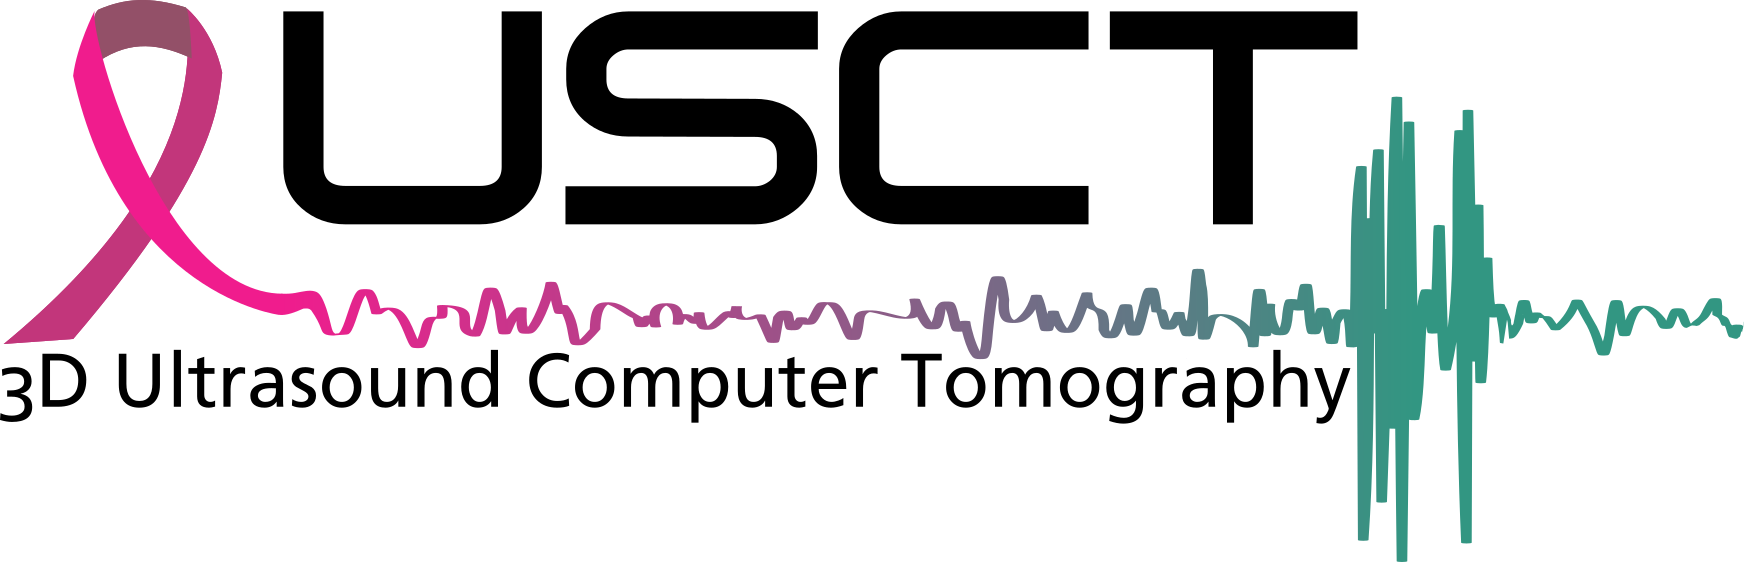
\includegraphics[width=4cm]{Graphics/USCT crowdfunding logo_frutiger_FINAL.png} }

   \vspace{3cm}


\begin{minipage}[c]{15.5cm}
\begin{center}
   \begin{huge}
   \hspace{-1cm}
     Extension and Evaluation of Tissue Classification\\
   \hspace{-1cm}
     Based on a Backscattering Model for\\
   \hspace{-1cm}
      3D Ultrasound Computer Tomography\\
   \end{huge}
\end{center}
\end{minipage}
\vfill
\begin{minipage}[c]{15.5cm}
   \begin{center}

    {\Large
     \ifenglish
     Master Thesis
 	\else
    Masterarbeit
	\fi
	}\\

    \vspace{0.5cm}
     {\large
      \ifenglish
        submitted by
      \else
        vorgelegt von
      \fi
      }\\
    \vspace{0.5cm}
     \textbf{\Large Benedikt Ebener}
   \vspace{4cm} \\


 \textsc{
 \ifenglish
   Institute for Data Processing and Electronics\\
   % choose appropriately
   Karlsruhe Institute of Technology\\
 \else
    Institut f\"ur Biomedizinische Technik\\
    % entsprechend auswählen
    Prof. Dr. rer. nat. Olaf D\"ossel / Prof. Dr. rer. nat. Werner Nahm / Dr.-Ing. Axel Loewe\\
    Korreferent: Prof. Dr. rer. nat. Olaf D\"ossel / Werner Nahm / Dr.-Ing. Axel Loewe\\
    Karlsruher Institut f\"ur Technologie\\
 \fi
 }

 \vspace{0.5cm}
 \ifenglish
  Reviewer: PD Dr. habil. Nicole Ruiter  \\
  Second reviewer: Prof. Dr. Marc Weber\\
  Advisor: Dr. Torsten Hopp 
 \else
   Betreuer: der Betreuer\\
 \fi
 
 \vspace{0.5cm}
5\textsuperscript{th} March  2021




  \end{center}
 \end{minipage}
\end{titlingpage}

\thispagestyle{empty}

\clearemptydoublepage
\newpage
\thispagestyle{empty}

\rmfamily
\vspace*{15cm}
{\setlength{\parindent}{0pt}

 \ifenglish
\textbf{Statutory declaration}\\\\
I declare that I have authored this thesis independently, that I have not used other than the declared sources/resources, and that I have explicitly marked all material which has been quoted either literally or by content from the used sources.

\vspace{1cm}

\makeatletter
\let\Date\@date
\makeatother

Karlsruhe, 5\textsuperscript{th} March  2021  % be changed to the date of the official end of the thesis

\hspace{1cm}

\closing{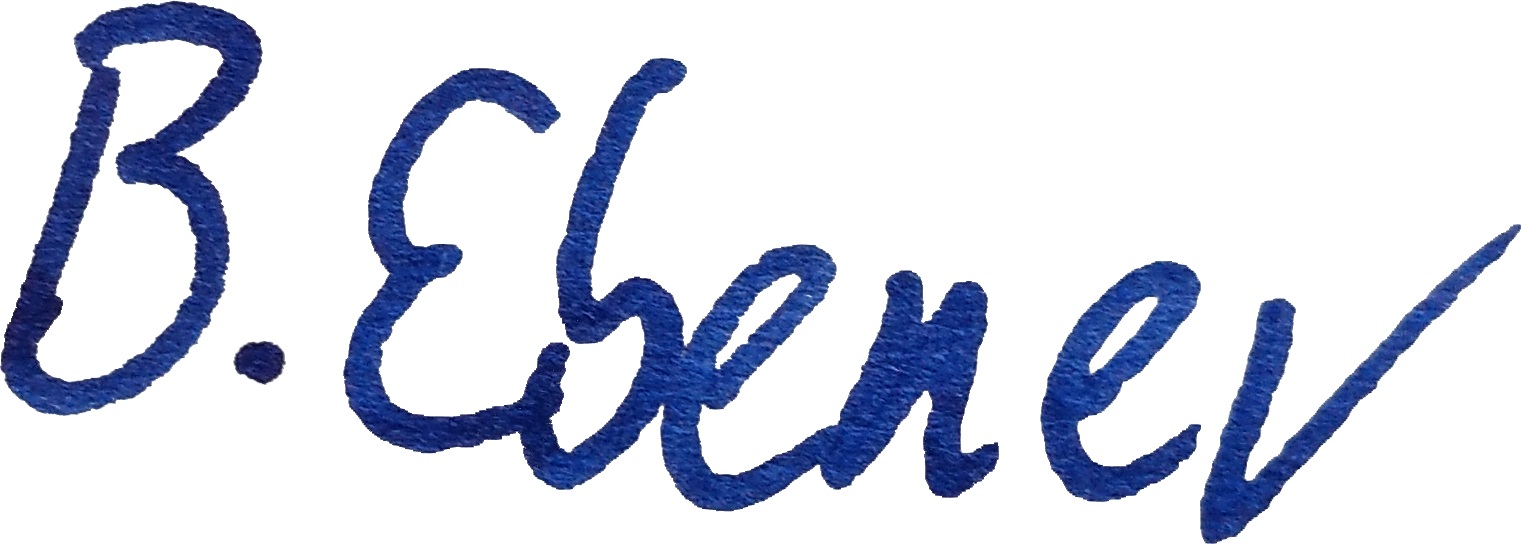
\includegraphics[height=1cm]{Unterschrift.png}}



\else
\textbf{Eidesstattliche Erkl\"arung}\\\\
Ich versichere wahrheitsgem\"a\ss{}, die Arbeit selbstst\"andig angefertigt, alle
benutzten Hilfsmittel vollst\"andig und genau angegeben und alles kenntlich gemacht zu haben,
was aus Arbeiten anderer unver\"andert oder mit Ab\"anderungen entnommen wurde.

\vspace{1cm}

Karlsruhe, den \today % this may also be changed to the date of the official end of the thesis
\fi

\fi
\frontmatter

\rmfamily
\setcounter{tocdepth}{2}
\addtocontents{toc}{\protect\thispagestyle{empty}}


%!TEX root = ../thesis.tex
\chapter*{Abstract}
\addcontentsline{toc}{chapter}{Abstract}
The abstract is a small summary of the thesis in approximately one a page. It must be written in English.\\
There should be a few words about the motivation for this research project, a short summary of the methods used and the most important results should be included also.\\
The abstract is meant for a future reader that wants to quickly find out if this work is relevant for him/her.


\clearemptydoublepage


%!TEX root = ../thesis.tex
\chapter*{Acknowledgments}
\addcontentsline{toc}{chapter}{Acknowledgments}
\markboth{Acknowledgments}{Acknowledgments}


Ich möchte die Gelegenheit nutzen und den vielen Menschen danken, die mich bei meiner Masterarbeit und meinem Studium unterstützt haben. Mein besonderer Dank gilt meinem Betreuer Torsten Hopp für die viele Zeit und die Mühen, die er aufgebracht hat, um mich bei den ganzen kleinen und großen Problemen während der Masterarbeit zu unterstützten. Darüber hinaus möchte ich mich für sein großartiges Feedback während der Korrekturphase bedanken. Bei Michael Zapf möchte ich mich ebenfalls bedanken für die Zeit, die er sich genommen hat und die vielen tollen Ideen, die zu großartigen Ergebnissen geführt haben.  Ebenfalls möchte ich mich bei Nicole Ruiter für die herzliche Unterstützung und ihren Rat bedanken.
Allen Mitarbeitern und Doktoranden am IPE möchte ich für die schöne gemeinsame Zeit danken, die wir trotz der Pandemiesituation miteinander verbringen durften. Nicht zuletzt möchte ich mich bei meinen Eltern Barbara und Frank für die emotionale, finanzielle und kulinarische Unterstützung während meines gesamten Studiums bedanken.
\clearemptydoublepage
\tableofcontents*
\clearemptydoublepage

\chapter*{Abbreviations}
\thispagestyle{empty}
\addcontentsline{toc}{chapter}{Abbreviations}
\markboth{Abbreviations}{Abbreviations}
\printacronyms[heading=none]
\clearemptydoublepage

\chapterstyle{madsen}
\ifafive  % right margin too small to have chapter numbers there
  \renewcommand*{\printchapternum}{%
    \hspace{0.4em}%
      \resizebox{!}{4ex}{%
        \chapnamefont\bfseries\sffamily\thechapter}%
  }%
\fi

\mainmatter
%!TEX root = ../thesis.tex
\chapter{Introduction}
\label{chap:introduction}


The last couple of decades have shown a steady increase of the incidence for female breast cancer.
An US based study published in March 2020 \cite{Lima2020Trends2015} has shown that the cancer incidence for women between the age of 25 to 39 has increased by 0.65\% per year. In 1935 the incidence for breast cancer was at 16.3 diagnoses per 100.000 women whereas 38.5 per 100.000 women were diagnosed in the year 2015.
In Germany 71.600 women were diagnosed with breast cancer in the year 2013 with cases having doubled since 1970. A more fortunate development has been observed in the death rate in patients diagnosed with breast cancer. Since 1999 the mortality rate decreased by about a third in patients under 50 and was 25\% lower in patients between the age 50-69 during that 14 year period.
Some of the various reasons for the increased incidence are presumably the higher age at which women become pregnant for the first time, hormone based birth control as well as a change in diet and in exercise \cite{RobertKoch-Institut2016Bericht2016}.
One of the reasons that the mortality rate could be decreased is the in the years 2005-2009 introduced  regular screening program for women between the ages 50-69. Since then the number of diagnosis of advanced tumour stages were decreased \cite{RobertKoch-Institut2016Bericht2016}.
The prognosis for the treatment of the cancer depends on the stage of the cancer and how early it was discovered. Furthermore, it has to be assessed whether the tumour might have spread into other organs so far. As the mortality rate directly correlates with the tumour size and stage of the cancer, an early detection of cancerogenous tissue is one of the most effective ways to increase the survivability of patients \cite{Veronesi1985PrognosisNodes}, \cite{Welch2016Breast-CancerEffectiveness}.

Among others some of the first symptoms of breast cancer often are changes in size or form of the breast as well as the formation of lumps within the breast  \cite{NationalInstitutesofHealthNIH-NationalCancerInstituteNCIBreastTreatment}.
The female breast consists of mainly fatty tissue and the mammary glands also known as lobules which produce milk occasionally during but mostly after pregnancy. Additionally, the ducts (see figure \ref{anatomy_breast}) are part of the breast tissue which form the transportation channels for the milk between the lobules and the nipple.
A very common type of breast cancer arises from this ductal system of the breast. The first symptom known as Ductal Carcinoma are the calcification therefore the deposition of calcium in the tissue of these glands.
This is a prestage of breast cancer known as stage 0 and is detectable by early mammography screening \cite{brestcancer_stages}.  


\begin{figure}[H]
    \centering
    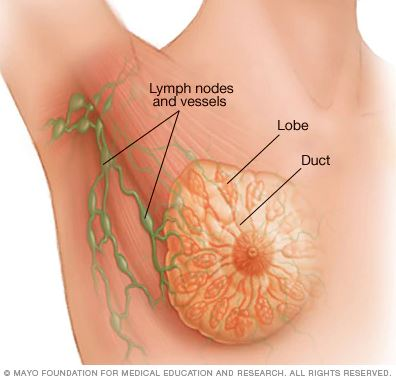
\includegraphics[width=0.75\textwidth]{Graphics/breast.jpg}
    \caption{Schematic of the female breast. The lobes form the milk producing system of the breast whereas the ducts are channels for the milk towards the nipple of the breast. Picture source: \cite{mayo-clinic}. }
    \label{anatomy_breast}
\end{figure}

\hspace{-1cm}
   
For the regular mammographic screenings typically X-ray-based imaging techniques are in use. The breasts has to be compressed between two plates so that a higher resolution of the breast tissue can be archived (see figure \ref{mammo_example_picture}). Besides the advantages of delivering results shortly after the screening and by having a high enough resolution to detect small tumour cells before they are detectable by palpation, there are certain downsides that have to be considered.
The biggest problem with X-ray-based mammographic screenings is the usage of ionising radiation. When it comes to x-ray and gamma radiation there is no such thing as a safe dose. Every dose of ionizing radiation of for example a low-dose X-ray mammography has proven to add to the incidence of breast cancer  \cite{Pauwels2015BreastRadiobiology} and so the main objective is the reduction of exposure to ionizing radiation.

\begin{figure}[H]
    \centering
    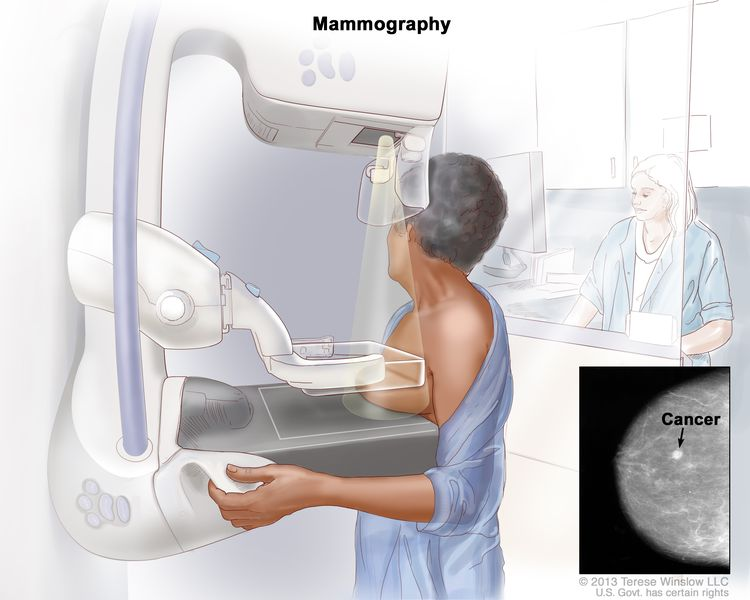
\includegraphics[width=0.75\textwidth]{mammography.jpg}
    \caption{Schematic of the mammography procedure. The breast is pressed between two plates and a beam of X-Ray-Radiation is used to produce the picture. On the bottom right is an example image of a female breast with the white dot indicating cancerogenous tissue. Picture source: \cite{NationalInstitutesofHealthNIH-NationalCancerInstituteNCIBreastTreatment}. }
    \label{mammo_example_picture}
\end{figure}

Another screening method is the physical examination of the breast either by the patient herself or during a clinical breast exam performed by a health professional. For this method the breast is carfully palpated to look for lumps or any kind of anomaly that might indicate an early stage of breast cancer. This method has one mayor disadvantage: lumps can only be detected by palpation after they have reached a certain size which, compared to the size of detectability during a mammography screening, is relatively large. Thus, the potential diagnosis of breast cancer solely by palpation often leads to the identification of first cancer symptoms in a later stage compared to mammography or \ac{usct} screening.   


Compared to the widely used X-ray-based screening method which uses ionizing radiation the three dimensional \ac{usct} has its advantages and makes this novel imaging technique a promising alternative to classical mammography. By utilizing the ultrasound echo technique high resolution 3D image of the breast tissue can be yielded without the use of ionizing radiation. Furthermore, the examination process with an \ac{usct} is much more comfortable for the patient since the breast does not have to be deformed during the imaging procedure. 




The total mastectomy is one of the possibilities to treat breast cancer. During this procedure big parts of the breast tissue as well as parts of the lymphatic system near the armpit are surgically removed (figure \ref{mastecto_example_picture}).  


\begin{figure}[H]
    \centering
    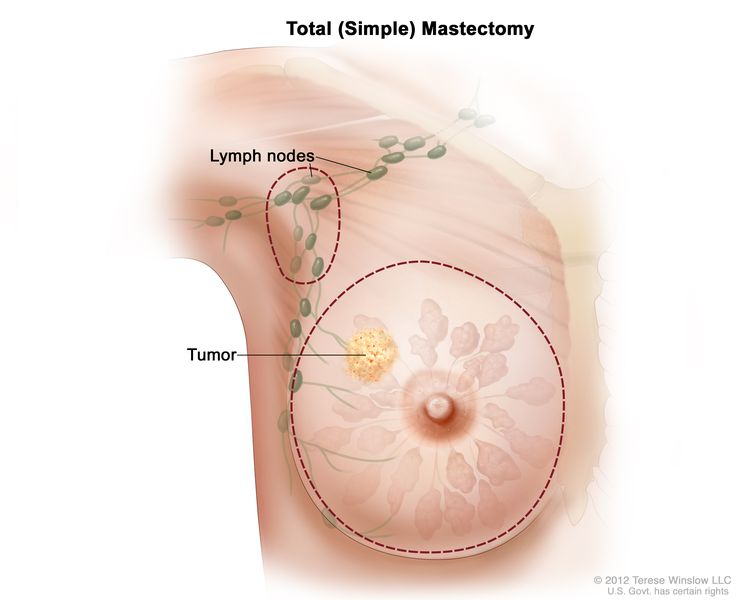
\includegraphics[width=0.75\textwidth]{Graphics/Mastectomy.jpg}
    \caption{Treatment of female breast cancer. During the mastectomy big parts of the breast are surgically removed (marked by dotted line). Picture source: \cite{NationalInstitutesofHealthNIH-NationalCancerInstituteNCIBreastTreatment}. }
    \label{mastecto_example_picture}
\end{figure}

This treatment may be combined with chemo therapy to decrease the size the tumour prior to the surgery. The post operative therapy often consists of radiation and hormone therapy to remove any cancer cells that might be left after the the mastectomy \cite{NationalInstitutesofHealthNIH-NationalCancerInstituteNCIBreastTreatment}.


\section{Motivation}

The goal of this thesis was to introduce a fourth modality to the reconstruction algorithm to further increase the resolution of the image as well as to classify different tissue types by analysing the back scattering. It is assumed that the tumour tissue consists of an inhomogeneous distribution of cancer cells which results in a distinct back scattering behaviour of the tissue.
By introducing the reflection characteristic algorithm to the reconstruction algorithm with an already implemented \ac{sos}-correction it is expected to further increase the clinical value of the reconstructed images as well as to make an assessment of the required computation power needed for the vast amount of data processing.



\clearemptydoublepage


%!TEX root = ../thesis.tex
\chapter{Medical Fundamentals}
\label{chap:medFund}


\section{Atrial Anatomy and Physiology}
\label{sec:anatomyPhysiology}

We try to support the diagnosis of arrhythmias like \ac{AFib}. \Ac{AFlut} already is very well understood.


\subsection{Electrophysiology}
\label{sec:anatomyPhysiology:elphy}

The course of an \ac{AP} is important to know.

\begin{figure}[tb]
 \centering
 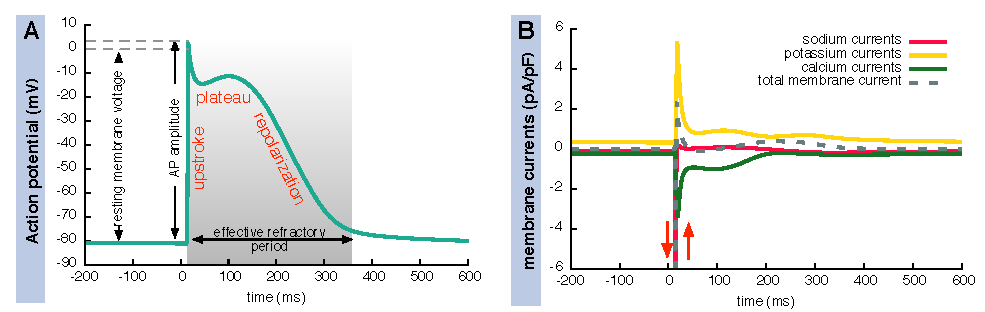
\includegraphics[width=\textwidth]{Funda-Med-AP}
 \caption{The course of the transmembrane voltage V$_\textnormal{m}$ during a cardiac \ac{AP} with its different phases (A) and the membrane currents carried by the different ions (B). The sodium current reaches an amplitude of $\approx$--70\,pA/pF. The calcium exchange with the sarcoplasmic reticulum is not considered. Courses were computed using the Courtemanche \etal model~\cite{courtemanche98}. Figure inspired by~\cite{schmidt10a}.}
 \label{fig:med:AP}
\end{figure}

\begin{figure}[ht]
\centering
\subfloat[Vector label (PDF format).]
	{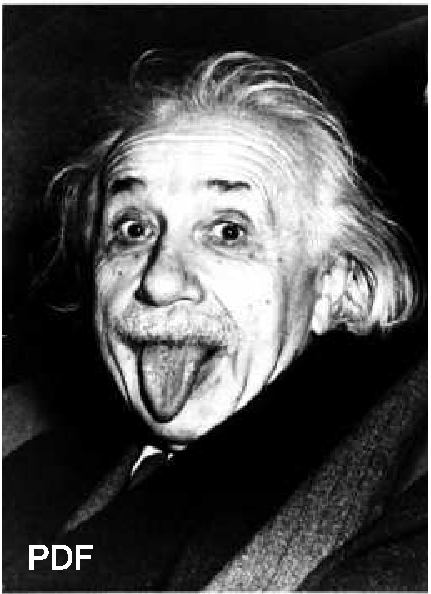
\includegraphics[width=0.4\textwidth]{einsteinlabelVEC}}
\hspace{0.05\textwidth}
\subfloat[Pixel label (PNG format).]
	{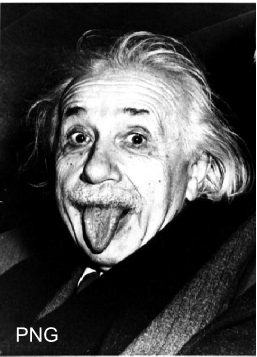
\includegraphics[width=0.4\textwidth]{einsteinlabelPIX}}
\caption{Photographs of different formats. One is vector~(a), one is pixel-base~(b).}
 \label{fig:med:einsteinComparsion}
\end{figure}

\Fig{fig:med:AP} is an example of a vector graphics figure. You can zoom in as you want, the figure will always stay sharp. This is the preferable format for all line drawings (\eg plots). Photographs are always saved as pixel graphics. However, labels can be added in a vector format (compare Figure~\ref{fig:med:einsteinComparsion}).\\
If you want to include a list of figures and a list of tables in your work, you probably want to provide short captions in square brackets as well. The

\clearemptydoublepage
%!TEX root = ../thesis.tex
\chapter{Mathematical Fundamentals}
\label{chap:mathFund}

Some mathematical formulas...\\
We establish the following transformations:
\begin{equation}
\label{eq:Fourier1}
F(u) = \frac{1}{N} \sum \limits_{x=0}^{N-1}f(x) e^{ -j 2 \pi \frac{u x}{N} }
  = \frac{1}{N} \sum \limits_{x=0}^{N-1}f(x) W_{N}^{ux}
\textrm{,}
\end{equation}
with $W_{N} = e^{ -j 2 \pi \frac{1}{N}} $ and $u=0,1,\dots,N-1$. Under the assumption of $N$ being..., \Eq{eq:Fourier1} can be expressed as...

\clearemptydoublepage


%!TEX root = ../thesis.tex
\chapter{Method A}
\label{chap:methA}

\section{Tables}
\label{sec:meth:tables}
Tables are a good way to present quantitative results. Mostly, they look best if you try to avoid vertical grid lines. \Tab{tab:meth:coverage} is an example of a table with a rather complex layout. \Tab{tab:meth:ionConcentrations} uses color to underline the structure and guide the eye. Decide for yourself what you like most and suits your needs best.
\begin{table}[tb]
\caption{Degree of coverage of RA elements with paths vulnerable to AFlut for different substrates and antiarrhythmic drugs. Some more description...}
\begin{center}
\begin{tabular}{lrrrcrrr}\toprule
& \multicolumn{7}{c}{\textbf{Degree of coverage}}\\ \cmidrule{2-8}
& \multicolumn{3}{c}{\textbf{Original CV}} & &\multicolumn{3}{c}{\textbf{Total activation time matched}} \\ \cmidrule{2-4} \cmidrule{6-8}
& no drug & amiodarone & dronedarone & & no drug & amiodarone & dronedarone \\ \midrule
\textbf{Control} & 18.1\% & 70.5\% & 0.0\% & & 18.1\% & 0.0\% & 0.0\% \\
\textbf{cAF} & 96.0\% & 96.3\% & 95.6\% & & 96.2\% & 96.1\% & 94.9\% \\
\textbf{N588K} & 93.2\% & 94.1\% & 0.0\% & & 93.0\% & 77.8\% & 0.0\% \\
\textbf{L532P} & 96.2\% & 96.5\% & 34.5\% & & 96.3\% & 96.0\% & 11.1\% \\
\bottomrule
\end{tabular}
\end{center}
\label{tab:meth:coverage}
\end{table}

\begin{table}[tb]
\caption[Ion concentrations and Nernst potential]{Typical concentrations and Nernst potentials of ions in a muscle cell.}
\centering
\begin{tabular}{>{\columncolor{lightBlue}}cccc}
  \toprule\rowcolor{lightBlue}
  \textbf{Ion}& \multicolumn{2}{c}{\textbf{Concentration ($mmol/kg\,H_2O$)}} & \textbf{Nernst}\\ \rowcolor{lightBlue}
  \textbf{type}& intracellular & extracellular & \textbf{potential} (mV)\\\rowcolor{lightBlue}
  \midrule
  $K^{+}$&\cellcolor{lightYellow} 4.5 &\cellcolor{lightYellow} 160 &\cellcolor{lightYellow} --95.4\\
  $Na^{+}$&\cellcolor{darkWhite} 144 &\cellcolor{darkWhite} 7 &\cellcolor{darkWhite} 80.2\\
  $Ca^{2+}$&\cellcolor{lightYellow} 1.3 &\cellcolor{lightYellow} 1e-5~to~1e-4 &\cellcolor{lightYellow} 126.5~to~157.3\\
  $Cl^{-}$&\cellcolor{darkWhite} 114 &\cellcolor{darkWhite} 7 &\cellcolor{darkWhite} --74.5\\
  \bottomrule
\end{tabular}
\label{tab:meth:ionConcentrations}
\end{table}


\section{Algorithms}
\label{sec:meth:algorithms}
\begin{algorithm}[tb]
\caption{The fast marching method. $\mathcal{N}\left(X\right)$ denotes the neighborhood of $X$.}
\begin{algorithmic}
\While{$TRIAL \neq\emptyset$}
  \State $X \gets \argmin_{X\in TRIAL}\left\{t_a\left(X\right)\right\}$
  \State $TRIAL \gets TRIAL\setminus\{ X\}$
  \State $KNOWN \gets KNOWN \cup \left\{ X \right\}$
  \ForAll{$\left(X_i \in \mathcal{N}\left(X\right) \right) \land \left( X_i \notin KNOWN \right)$}
    \State $t_a\left(X_i\right) \gets$ update$\left(X_i,X\right)$
    \If{$X_i \notin TRIAL$}
      \State $TRIAL \gets TRIAL \cup \left\{X_i\right\}$
    \EndIf
  \EndFor
\EndWhile
\end{algorithmic}
\label{alg:meth:fastMarching}
\end{algorithm}Algorithms in pseudo code can be defined using the \textit{algorithmicx} package: \url{https://www.ctan.org/tex-archive/macros/latex/contrib/algorithmicx/}. \Alg{alg:meth:fastMarching} gives an example.

\section{References}
\label{sec:meth:references}
To reference conveniently and consistently to chapters, sections, figures, tables, algorithms, equations and so on, we defined some macros:\\
\begin{itemize}
  \item In \Chap{chap:medFund}
  \item In \Sec{sec:anatomyPhysiology}..., in \Sec{sec:anatomyPhysiology:elphy}
  \item In \Fig{fig:med:AP}
  \item In \Tab{tab:meth:coverage}
  \item In \Alg{alg:meth:fastMarching}
  \item Under the assumption of equal anisotropy ratios, \Eq{eq:Fourier1} can be transformed into...
\end{itemize}

\subsection{Literature References}
\label{sec:meth:references:literature}
Regarding literature references, our reference management system \textit{refbase} already covers a good share of relevant literature. The \textit{refbase} entries are exported into a \textit{bibtex} file on the \textit{bordeaux} disk once every night: \textit{/Volumes/bordeaux/bibtex/export.bib}. In the template archive, there is a file \textit{refbase.bib} linking to the correct path on \textit{bordeaux}. References from there can be cited conveniently using the cite key, e.g.~\cite{courtemanche98}. When citing books, you should include the respective chapter~\cite[Chap. 5]{belytschko00} or pages  \cite[pp. 239--240]{belytschko00}. These specifications are not required when citing papers~\cite{riedel02}. You can switch between APA and IEEE citation style in \textit{config.tex}.\\
The best way to include additional literature is directly import it to refbase as described in our wiki: \url{https://intern.ibt.uni-karlsruhe.de/wiki/Introduction_to_Refbase}.\\
At some point you probably want to change some things manually. The preferable way is to do so directly in \textit{refbase}. If this is not possible, you need a local bibtex file. As the \textit{refbase} export comprises several hundreds of thousands of lines and several megabytes, opening it in a text editor can be tedious and cumbersome. Therefore, we have a script \textit{ExtractBibEntriesFromBBL.pl} that extracts the entries you actually used and combines them in a new and smaller bibtex file (recommended name: \textit{reduced.bib}). You just need to pass the \textit{.bbl} file that is created during the compilation of your \LaTeX\ document using \textit{refbase.bib} (usually \textit{thesis.bbl}). Then, you can edit the entries in your local \textit{reduced.bib} file according to your needs. By putting curly braces around one or several characters, you can force them to be included in your references listing the way you defined them, \eg \{P\}-wave. You should do the \textit{ExtractBibEntriesFromBBL.pl} step towards the end of your writing when you feel that you won't include a lot more references. Running the script again will overwrite your local changes. Therefore, the easiest way to include additional references is to produce the bibtex entry right from the \textit{refbase} web interface and paste it into your local \textit{reduced.bib}.

\section{Abbreviations}
The acronym package helps you to keep track of abbreviations. See also \textit{abbreviations.tex} and \url{https://www.ctan.org/pkg/acronym}.
\cite{EKGO}

\clearemptydoublepage


\chapter{Results}
\label{chap:results}




\section{Experimental Setup}
\label{sec:input_data}


For the evaluation of the algorithm a suitable data set of a setup with a simple object with a smooth, organic surface was chosen. The following data set '\code{exp0040\_Carina\_\-PhantomGelatineOlive\-\_mitHalterung}' fulfils these requirements \cite{Wittenbeck2017Konzeption3D-Ultraschalltomographie}. The acquired data resulted from an \ac{usct} measurement of a phantom consisting of an olive inside a gelatin block. For the imaging a phantom was placed into the \ac{usct} device. 
The measurement setup can be seen in Figure \ref{fig:gelatine_setup}:


\begin{figure}[H]
     \centering
     \begin{subfigure}[b]{0.49\textwidth}
         \centering
         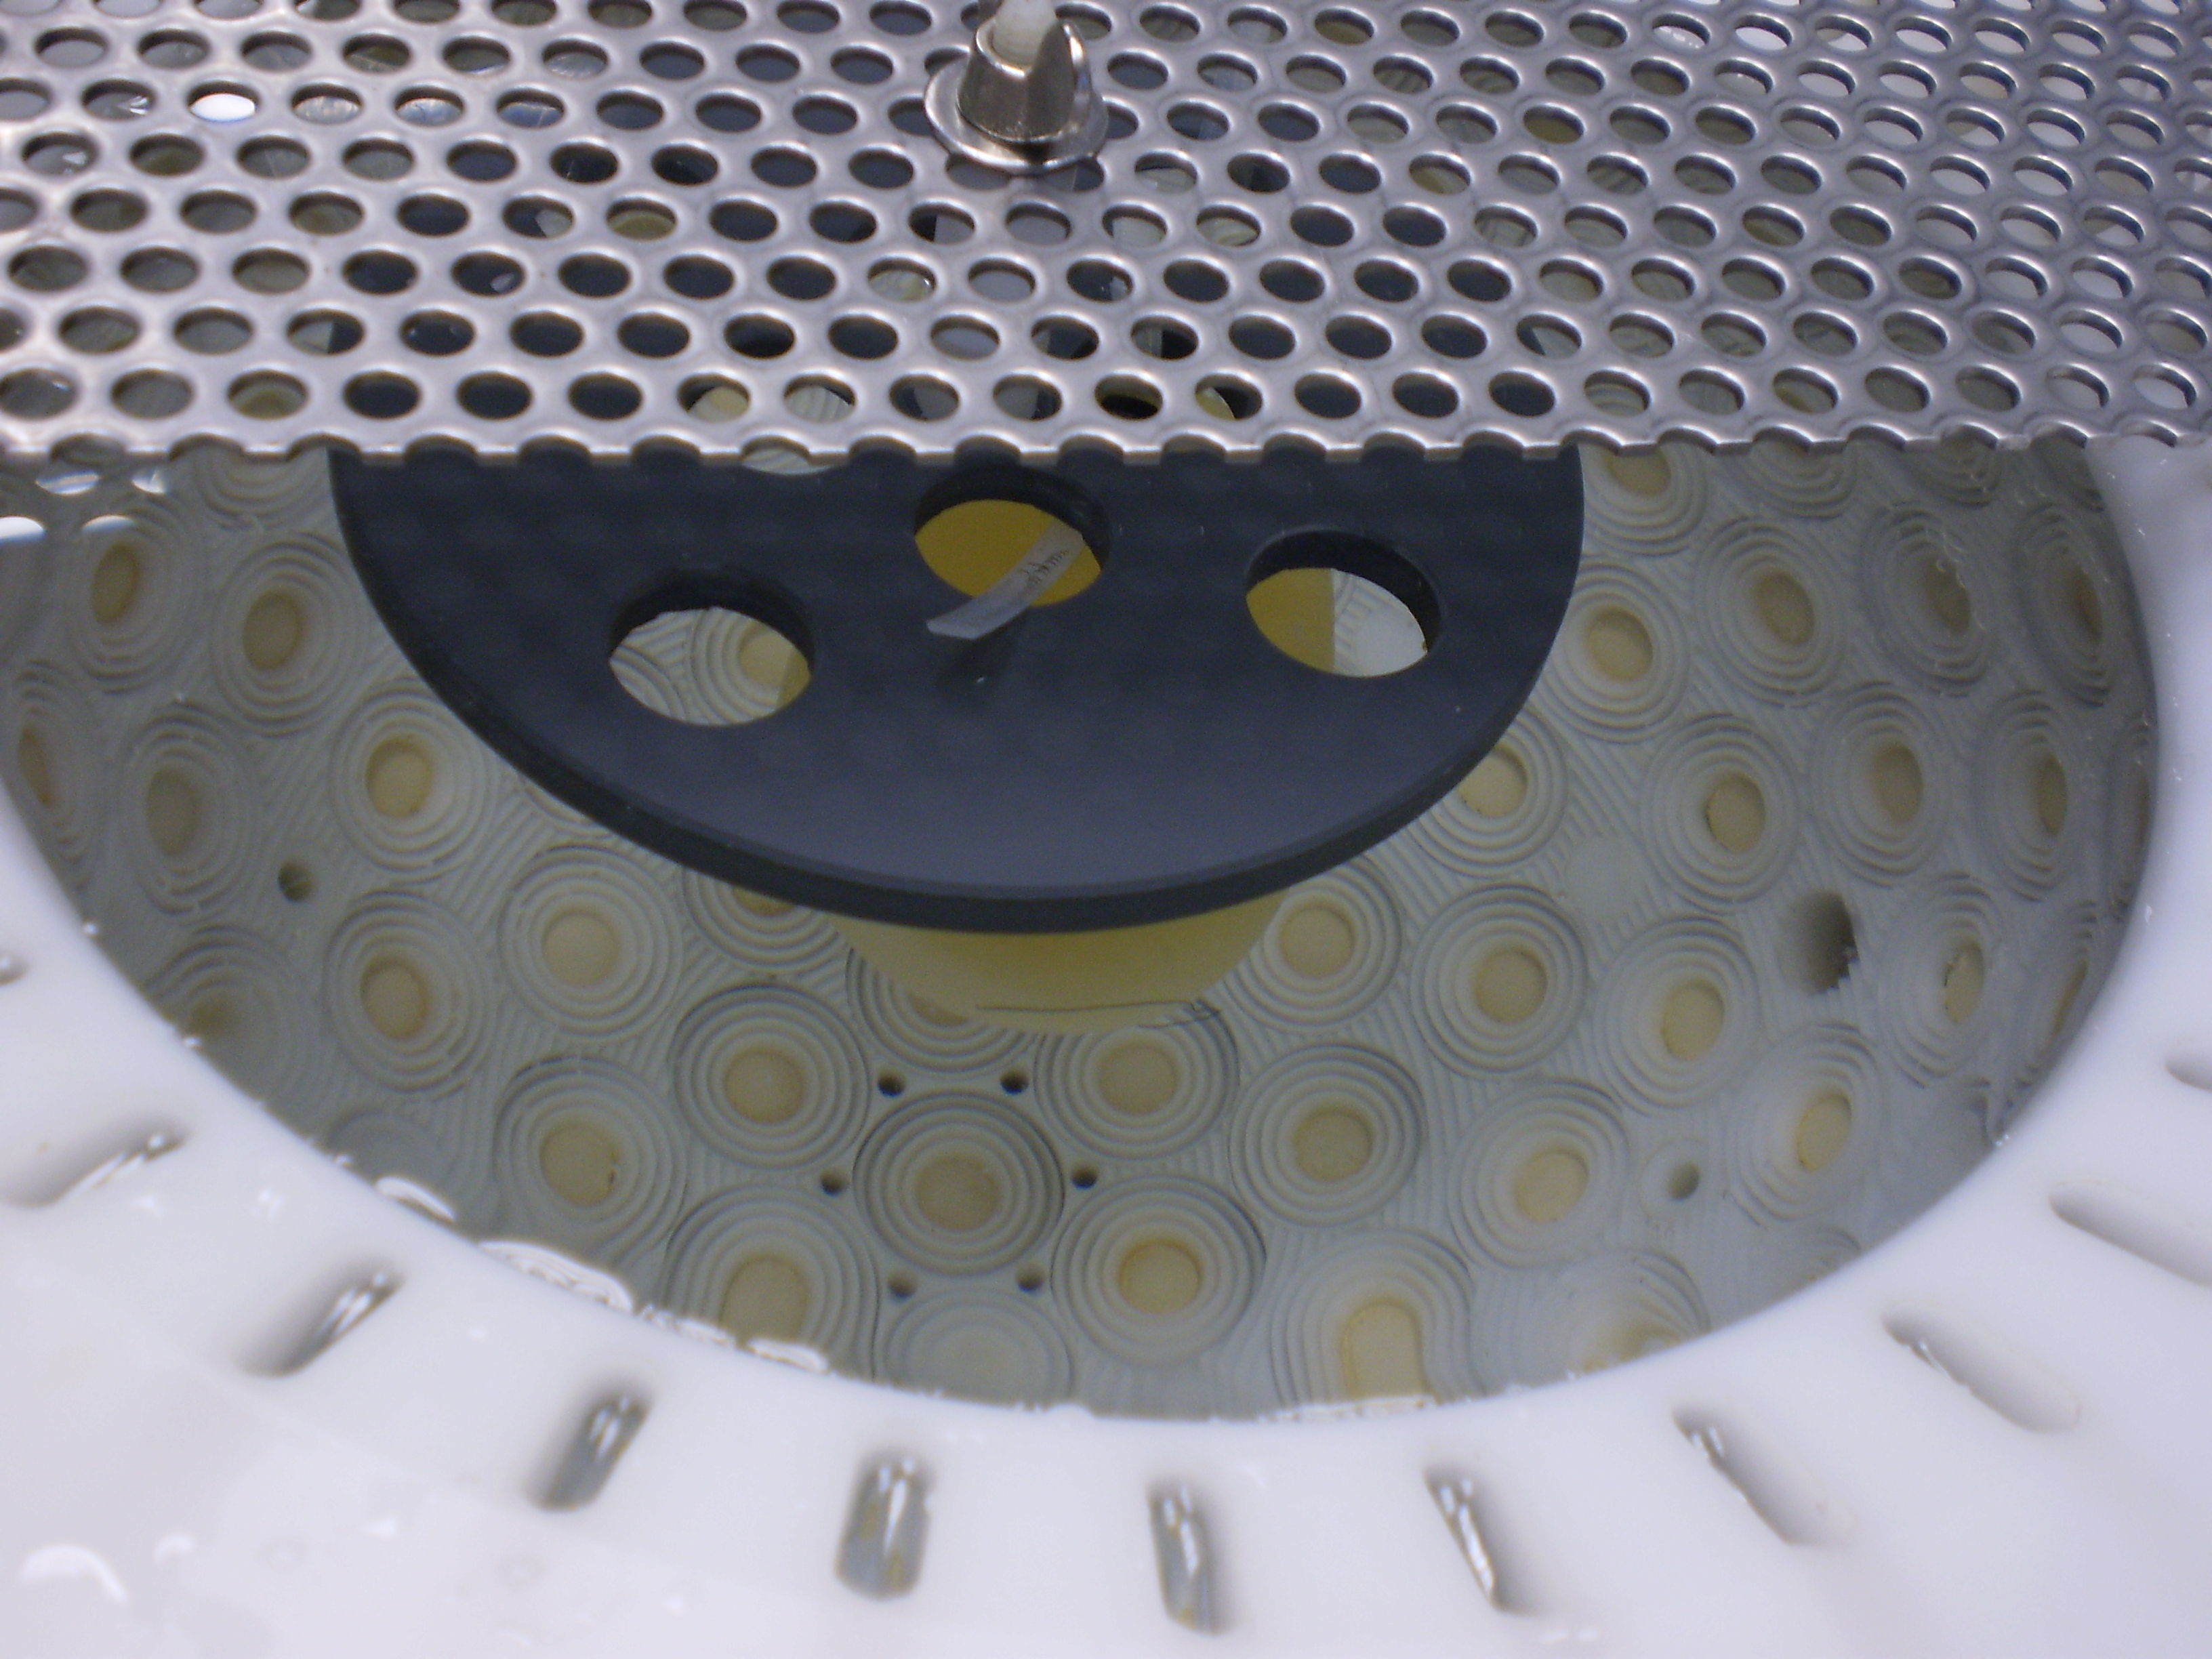
\includegraphics[width=0.99\textwidth]{Graphics/gelatin_setup1.JPG}
         \caption{Gelatin block in the imaging aperture of the \ac{usct} device.}
         \label{fig:gelatine_setup_2}
     \end{subfigure}
     \hfill
     \begin{subfigure}[b]{0.49\textwidth}
         \centering
         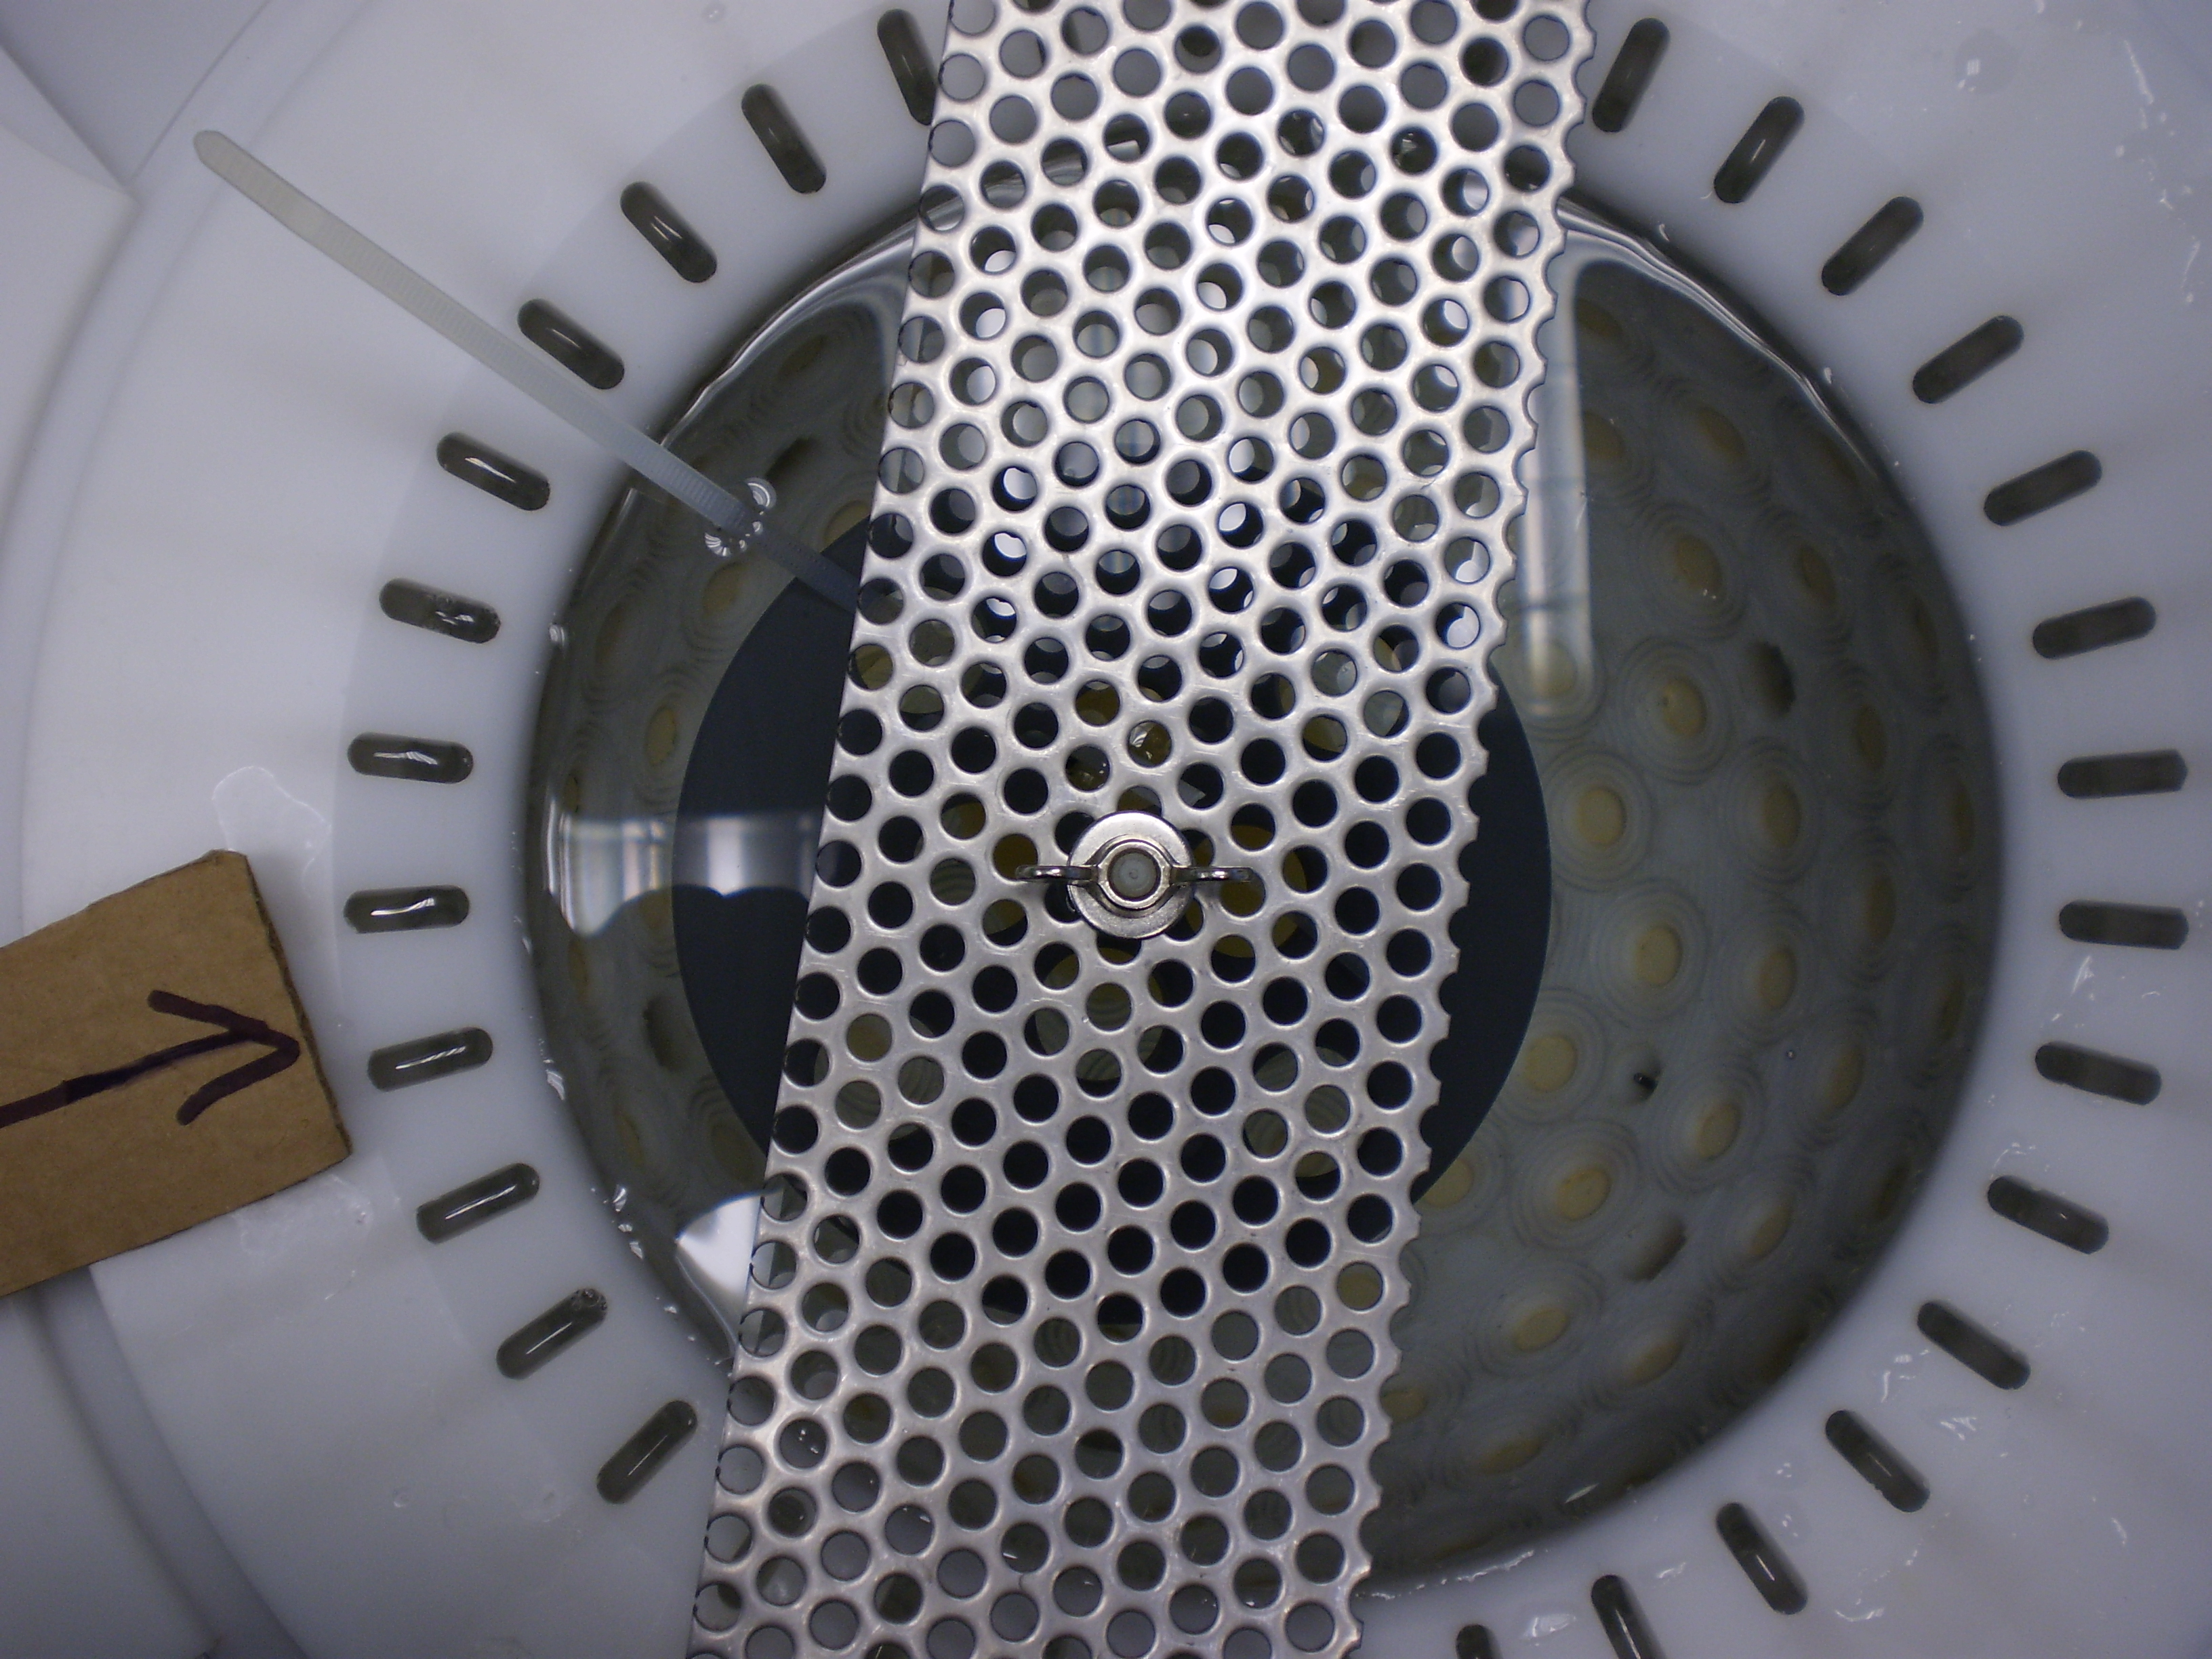
\includegraphics[width=0.99\textwidth]{Graphics/gelatin_setup 2.JPG}
         \caption{View from the top.}
         \label{fig:gelatine_setup_1}
     \end{subfigure}
        \caption{Measurement setup of the gelatin block with olive inside of the \ac{usct} device.}
        \label{fig:gelatine_setup}
\end{figure}


The \acp{ascan} were recorded for all 157 \ac{tas} with ten aperture positions so a total of $157\cdot4\cdot157\cdot9\cdot10 = 8.8\cdot10^6$ \acp{ascan} were recorded. The reconstructed reflection image for this data set is shown in Figure \ref{fig:res:reflec_image_olive_xyz}. The sub plots each show a slice through the image. The coloured lines in each plot show the selected slice in the other two coordinate systems. The blue marker belongs to the z-dimension, the green one corresponds to the y-dimension and the red marker shows the x-dimension. Figure \ref{fig:res:reflec_image_olive_xyz_x} shows the x-layer for $x = 0$. That x is equal to zero can be seen in the other two figures where the red markers are located at about 0. Analogously, Figure \ref{fig:res:reflec_image_olive_xyz_y} and  \ref{fig:res:reflec_image_olive_xyz_z} show the y-layer and z-layer of the image.

\begin{figure}[H]
     \centering
     \begin{subfigure}[b]{0.49\textwidth}
         \centering
        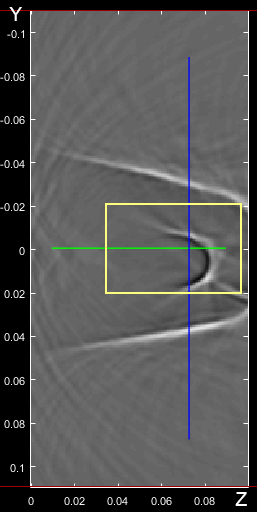
\includegraphics[width=0.59\linewidth]{Graphics/Results/Olive_Standart_reco_example/olive_standart_reconstruction_whole_volume_x_layer.png}
         \caption{x-Layer}
         \label{fig:res:reflec_image_olive_xyz_x}
     \end{subfigure}
     \hfill
     \begin{subfigure}[b]{0.49\textwidth}
         \centering
         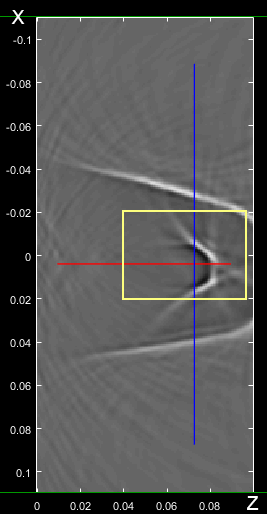
\includegraphics[width=0.61\textwidth]{Graphics/Results/Olive_Standart_reco_example/olive_standart_reconstruction_whole_volume_y_layer.png}
         \caption{y-Layer}
         \label{fig:res:reflec_image_olive_xyz_y}
     \end{subfigure}
     \hfill
     \begin{subfigure}[b]{0.55\textwidth}
         \centering
         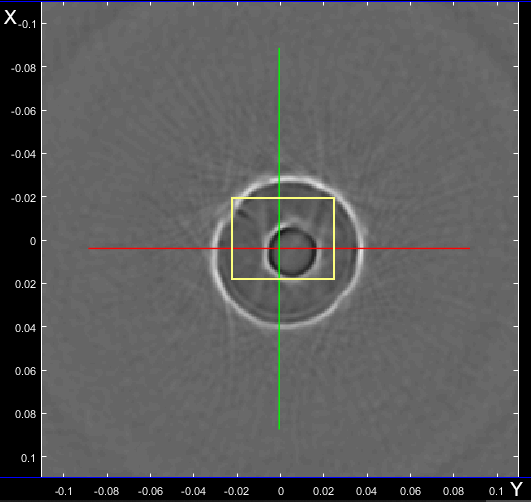
\includegraphics[width=0.99\textwidth]{Graphics/Results/Olive_Standart_reco_example/olive_standart_reconstruction_whole_volume_z_layer.png}
         \caption{z-Layer}
         \label{fig:res:reflec_image_olive_xyz_z}
     \end{subfigure}
        \caption{Reconstructed reflection image of an olive in gelatin. The yellow box marks the area that was used during the reconstructions with five dimension to limit the amount of data.}
        \label{fig:res:reflec_image_olive_xyz}
\end{figure}


In the centre of Figure \ref{fig:res:reflec_image_olive_xyz_z} the olive can be seen as the smaller, darker circular shape. The brighter shape around the olive is the gelatin block. 

\bigskip


The volume was only partially considered during the 5D reconstruction to reduce the amount of data that had to be processed and by that also reduce the computation time. The start point for the volume was set to $[\, -0.02,\, -0.02,\, 0.04\, ]$ and the end point was set to: $[ 0.02,\, 0.02,\, 0.095\, ]$. The volume considered in the analysis is marked with the yellow boxes in Figure \ref{fig:res:reflec_image_olive_xyz}. This particular volume was chosen to include as many different types of tissue as possible. Therefore, four particular voxels where chosen at the location of different tissue samples. The first voxel is located at $[85\, , \, 66\, , \, 87]$ at the edge of the olive. The 2\textsuperscript{nd} test voxel is located at $[18\, , \, 21\, , \, 87]$ right in the gelatin around the olive. The third voxel is located on the surface of the gelatin block at the coordinates $[1\, , \, 6\, , \, 76]$. At $[40\, , \, 60\, , \, 87]$ another voxel was chosen in the pulp of the olive. The position of these voxels can be seen in Figure \ref{fig:different_tisue_types}.  
      
      
      
\begin{figure}[H]
    \centering
    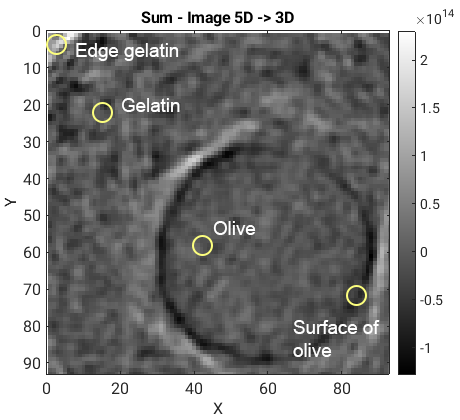
\includegraphics[width=0.76\textwidth]{Graphics/Results/Variance_Image/stone_skin_pulp_location.png}
    \caption{Overview of the reconstructed area with the location of the test voxels for the different materials inside of the imaging aperture.}
    \label{fig:different_tisue_types}
\end{figure}
    


\section{Evaluation of the assignment process during 5D reconstruction}
The introduction of the fifth dimension was explained in section \ref{chap:SAFT_Augment}. The assignment process of the  voxel value $V_k$ to the voxels in the 4\textsuperscript{th} and 5\textsuperscript{th} dimension was explained in section \ref{sec:index_ident}. The functionality of this process is verified in this section. In this example the 4\textsuperscript{th} dimension will relate to the comparison vector from the voxel to the receiver. The 5\textsuperscript{th} dimension is defined as the comparison vector from the voxel to the emitter. During the reconstruction 14 directional vectors were used. 
The configuration of active emitters and receivers is shown in Figure \ref{fig:res:5th_dim_over_4th_aperture}. The green crosses mark the location of all active receivers and the red circles represent the emitters. For this example the first 30235 \acp{ascan} are used which include the first 40 emitters and 1309 receivers. The data of every receiver that lays in a $\pm 120^{\circ}$ angle to the sender normal is included for that particular emitter.

\begin{figure}[H]
    \centering
    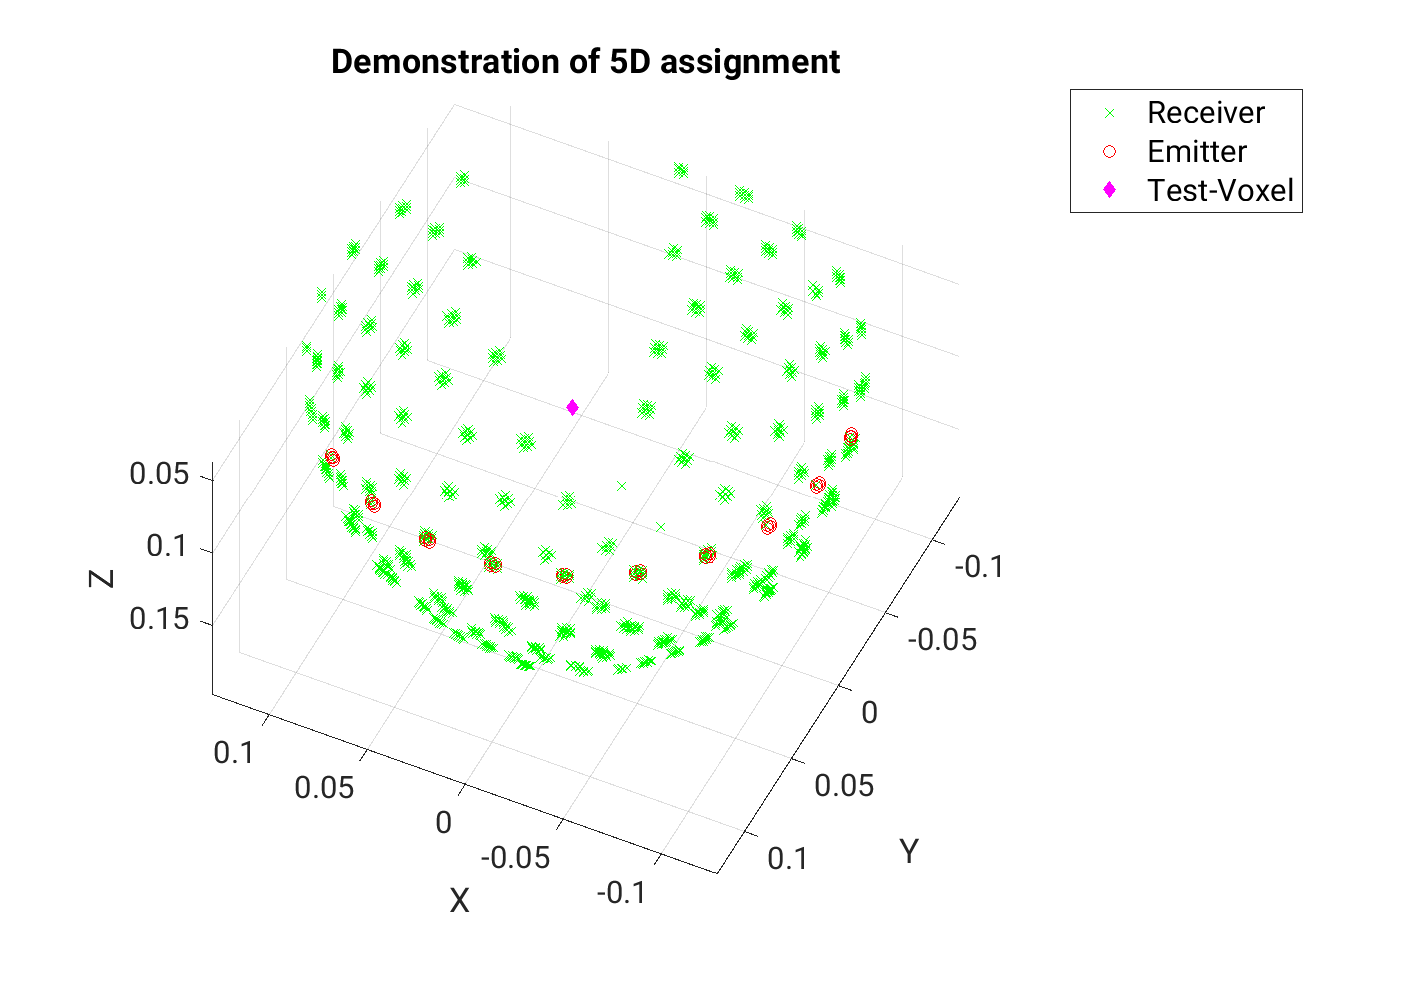
\includegraphics[width=0.89\linewidth]{Graphics/Results/4d_5d/5thDim_over_4thDim_150_150_150_apertur.eps}
    \caption{Configuration of 10 emitting and 145 receiving \ac{tas} and a test voxel in the centre of the aperture. The receivers are shown in green and the emitters as red circles. The units on the axes is given in meter. }
    \label{fig:res:5th_dim_over_4th_aperture}
\end{figure}

 For this example a test voxel is defined arbitrarily in the centre of the aperture. The coordinates of this point are given by voxel indices $[150\, , \, 150\, , \, 150]$ and it is shown as the pink diamond in Figure \ref{fig:res:5th_dim_over_4th_aperture}. The coordinates of the voxel can be converted into the coordinate system of the \ac{usct} which is given in meters. The test voxel therefore is located at $[0.0047m\, , \, 0.0047m\, , \, 0.0047m]$.

The following figure shows the voxel values for the one test voxel in the centre of the aperture at the position of the pink diamond. Since there are 5 dimensions each dimensions gets assigned a certain amount of voxel values for each combination of dimensions. Every combination of the 4\textsuperscript{th} dimension with the 5\textsuperscript{th} dimension is shown in Figure \ref{fig:res:5th_dim_over_4th_result}.
 
 
\begin{figure}[H]
    \centering
    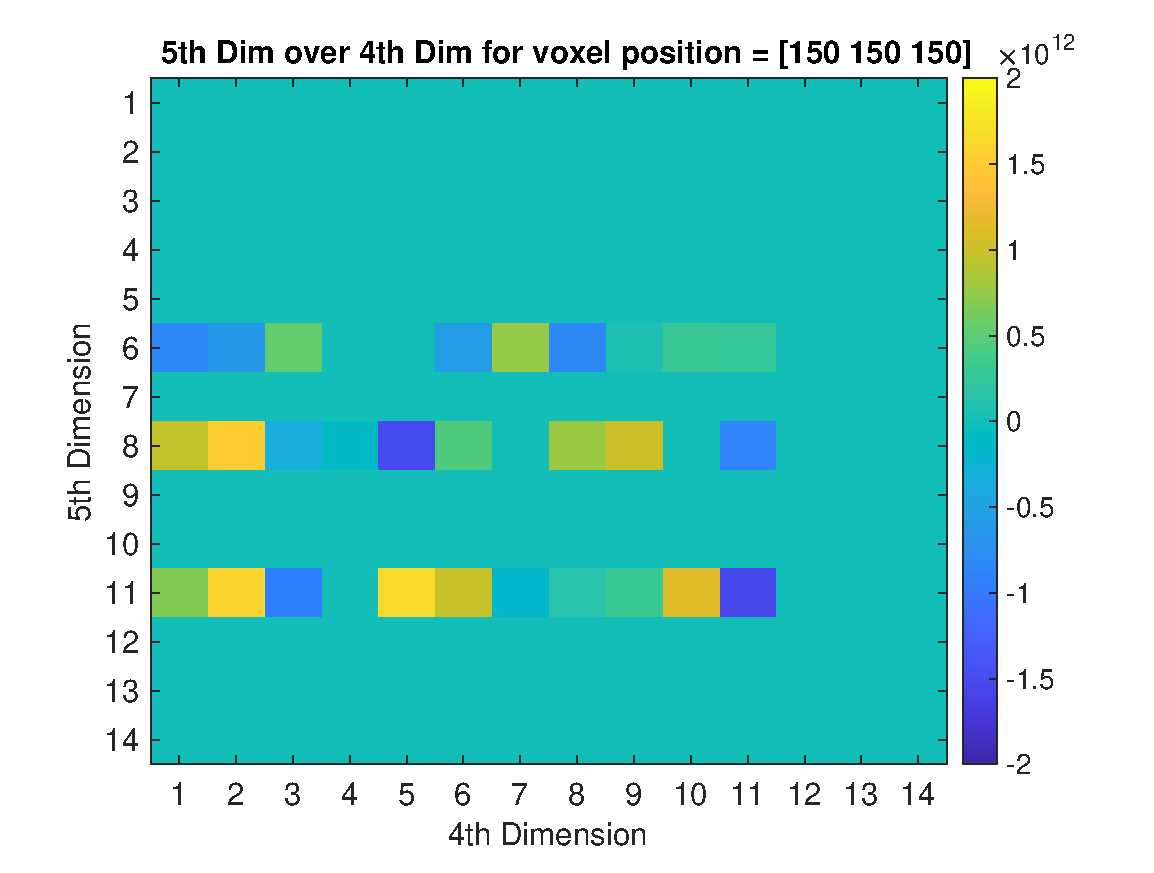
\includegraphics[width=0.89\linewidth]{Graphics/Results/4d_5d/5thDim_over_4thDim_150_150_150.eps}
    \caption{Resulting voxel values $V_k$ of the five dimensional reconstruction. The 4\textsuperscript{th} dimension relates to the voxel-receiver-vector. The 5\textsuperscript{th} dimension represents the directional information for the voxel-emitter-vector.}
    \label{fig:res:5th_dim_over_4th_result}
\end{figure}

To understand Figure \ref{fig:res:5th_dim_over_4th_result} the example of the Rubik's cubes in Figure \ref{5D_rubics} shall be used. In the previous example there were only four directional vectors. This resulted in $4 \times 4 = 16$ Rubik's cubes. In the 4\textsuperscript{th} dimension the cubes held the information about the receiver directions. The the 5\textsuperscript{th} dimension held the data for the emitters. The here shown data was generated with 14 directional vectors which leads to a $14 \times 14$ matrix with a total of 196 Rubik's cubes. These 196 Rubik's cubes are shown in Figure \ref{fig:res:5th_dim_over_4th_result} but not as whole but only the value of the voxel $[150\, , \, 150\, , \, 150]$ in each cube.
Every value that can be found in the same row of the matrix in Figure \ref{fig:res:5th_dim_over_4th_result} was recorded by the same emitter. Analogously, every value in the same column belongs to the same receiver. The distribution of values in the 5D-over-4D representation is compared to the emitter-receiver-configuration from Figure \ref{fig:res:5th_4th_cones}. It shows the 14 directional vectors and their corresponding decision cones.


\begin{figure}[H]
     \centering
     \begin{subfigure}[b]{0.49\textwidth}
         \centering
        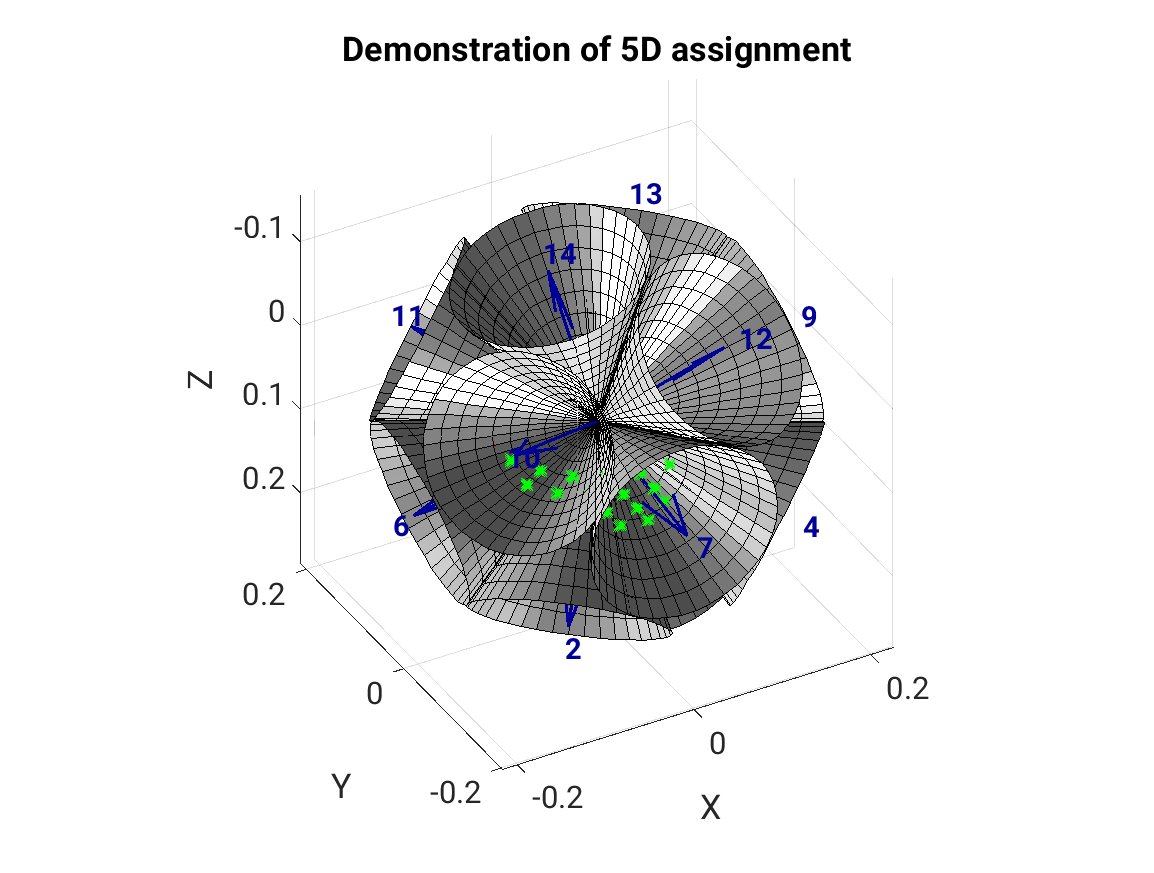
\includegraphics[width=1.3\linewidth]{Graphics/Results/4d_5d/5thDim_over_4thDim_150_150_150_cones_10_center.eps}
         \caption{Cone 10}
         \label{fig:res:5th_4th_cones10}
     \end{subfigure}
     \hfill
     \begin{subfigure}[b]{0.49\textwidth}
         \centering
         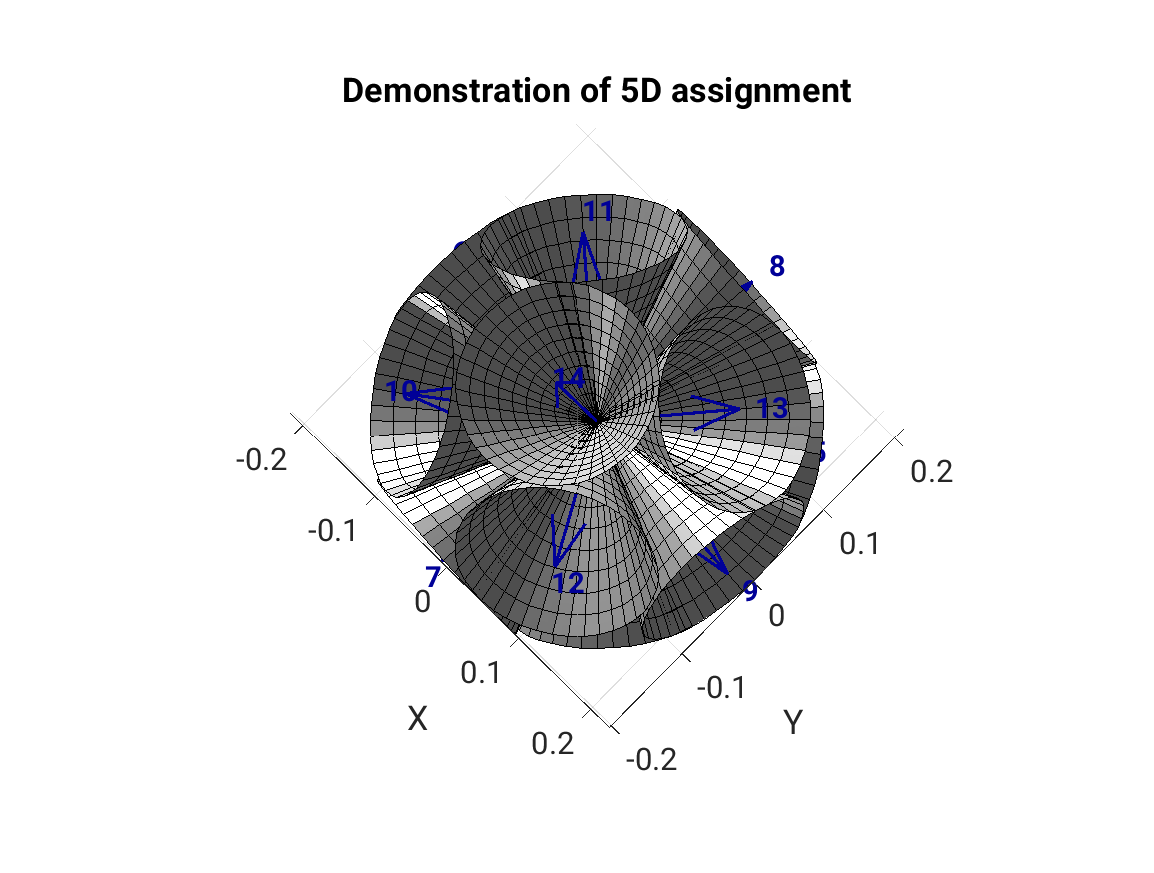
\includegraphics[width=1.3\textwidth]{Graphics/Results/4d_5d/5thDim_over_4thDim_150_150_150_cones_14_center.eps}
         \caption{Cone 14}
         \label{fig:res:5th_4th_cones14}
     \end{subfigure}
     \hfill
     \begin{subfigure}[b]{0.49\textwidth}
         \centering
         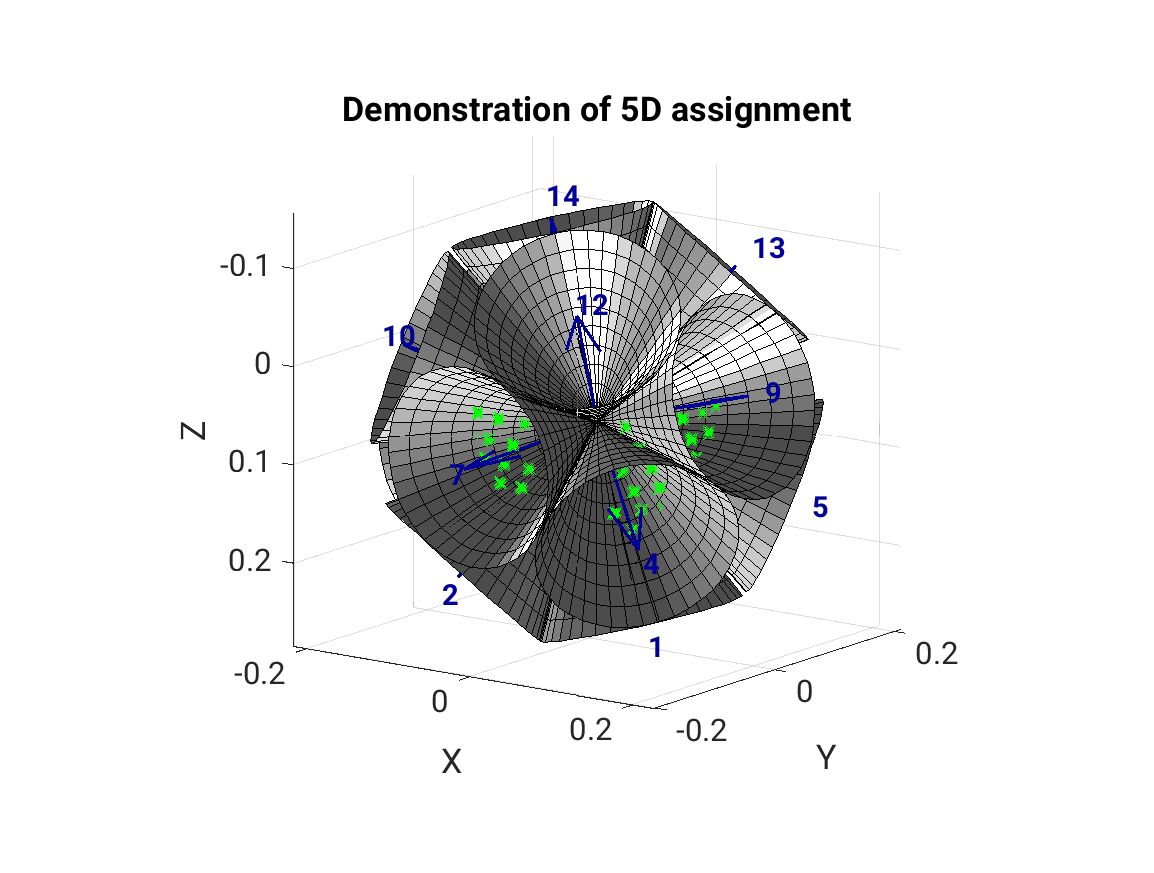
\includegraphics[width=1.3\textwidth]{Graphics/Results/4d_5d/5thDim_over_4thDim_150_150_150_cones_7_9_center.eps}
         \caption{Cone 12}
         \label{fig:res:5th_4th_cones12}
     \end{subfigure}
     \hfill
     \begin{subfigure}[b]{0.49\textwidth}
         \centering
         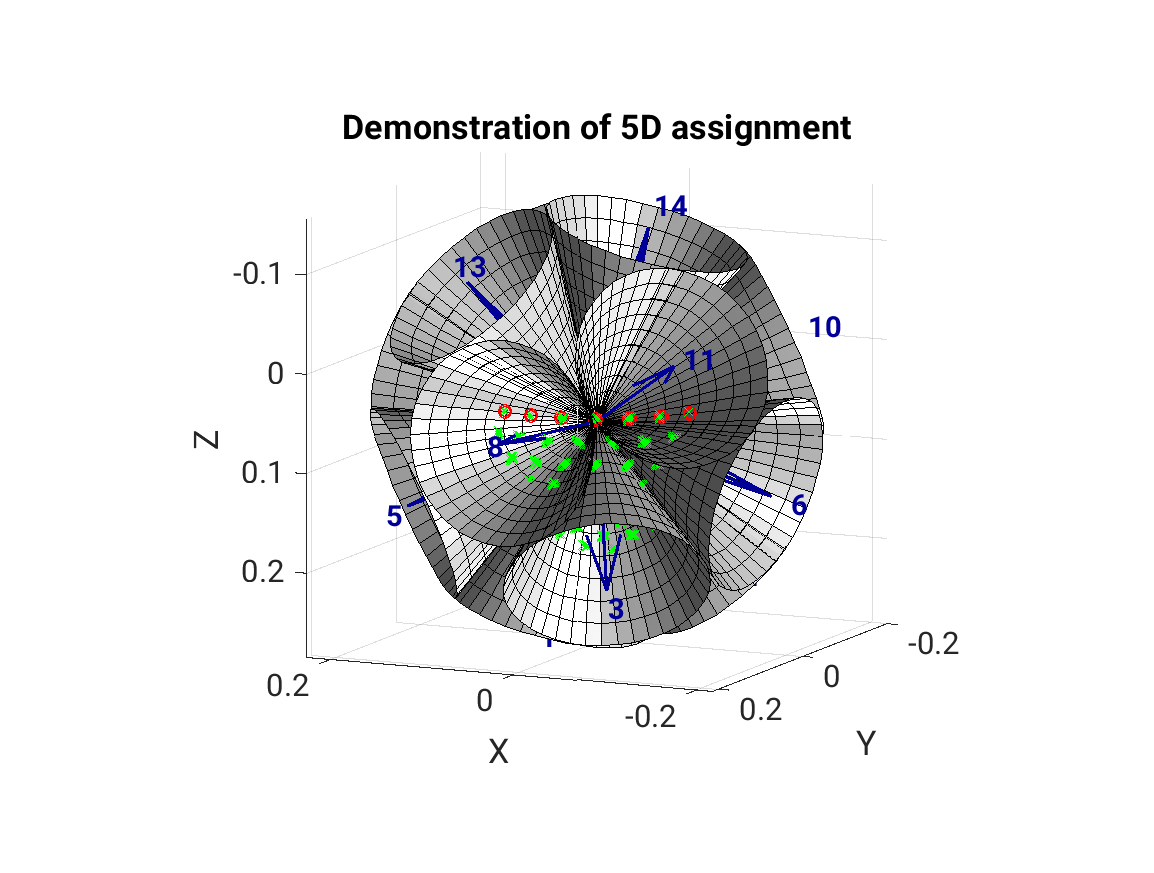
\includegraphics[width=1.3\textwidth]{Graphics/Results/4d_5d/5thDim_over_4thDim_150_150_150_cones_8_11_center.eps}
         \caption{Cone 11}
         \label{fig:res:5th_4th_cones11}
     \end{subfigure}
     \hfill
     \begin{subfigure}[b]{0.49\textwidth}
         \centering
         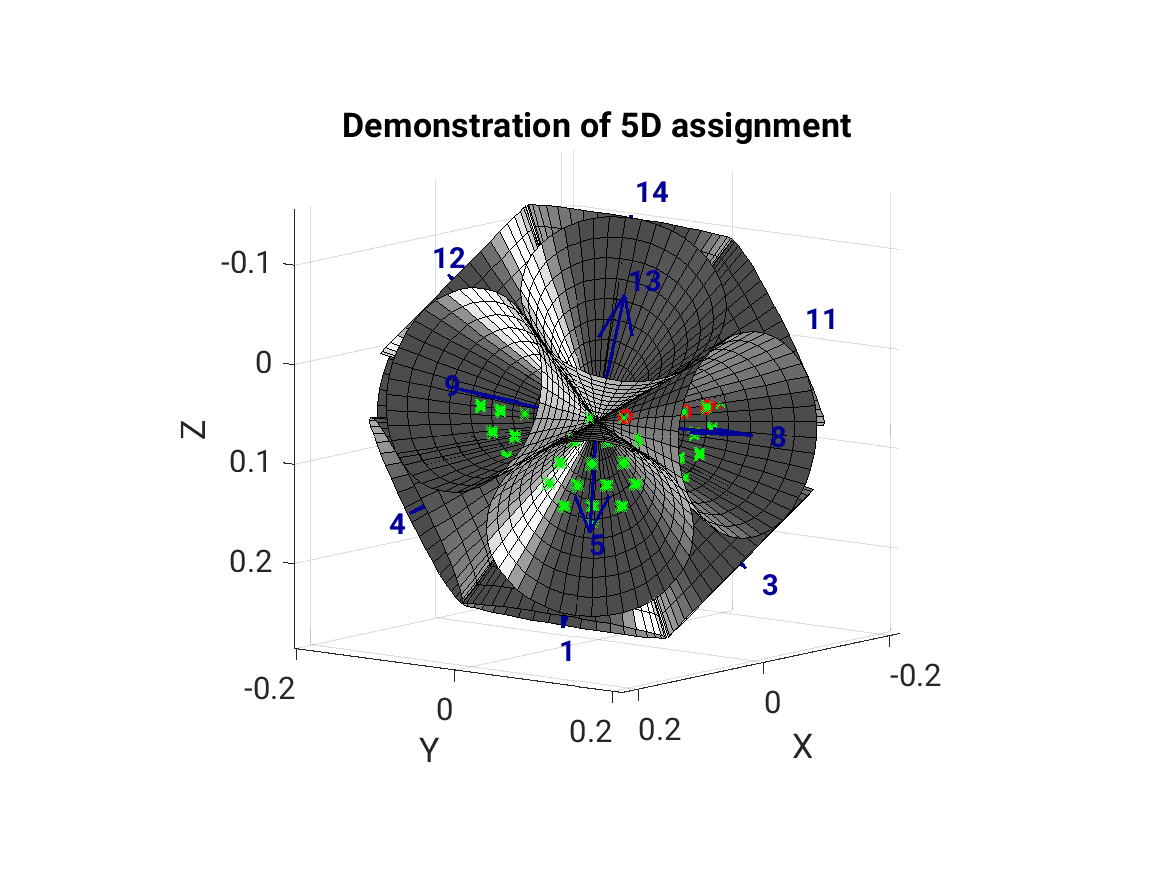
\includegraphics[width=1.3\textwidth]{Graphics/Results/4d_5d/5thDim_over_4thDim_150_150_150_cones_9_8_center.eps}
         \caption{Cone 5}
         \label{fig:res:5th_4th_cones5}
     \end{subfigure}
        \caption{The emitter receiver configuration of Figure \ref{fig:res:5th_dim_over_4th_aperture} with added directional vectors and decision cones. The origin of each cone is located at the position of the test voxel $[150\, , \, 150\, , \, 150]$. }
        \label{fig:res:5th_4th_cones}
\end{figure}

To connect the results shown in Figure \ref{fig:res:5th_dim_over_4th_result} with the cone images in Figure \ref{fig:res:5th_4th_cones} we will begin with the interpretation of the the emitter information. The emitters that were used are represented by the red markers in Figure \ref{fig:res:5th_4th_cones}.   

The cones show the decision areas of each directional vector. If a emitter position can be seen inside of a cone (i.e. a red dot is visible in the cone) the voxel values $V_k$ originating from that emitter are assigned to the directional vector of that cone.  

In this example the following cones contain emitter positions: 6, 8 and 11. The results in Figure \ref{fig:res:5th_dim_over_4th_result} show that only the rows for corresponding to emitters 6, 8 and 11 are occupied. All other rows are empty. This coincides with the assumption that the 5\textsuperscript{th} dimension relates to the voxel-emitter directional information the voxel values are only assigned to the corresponding emitter cones.

For the receivers, which are plotted in green, the data is stored in the 4\textsuperscript{th} dimension of Figure \ref{fig:res:5th_dim_over_4th_result}. This coincides with the representation in Figure \ref{fig:res:5th_dim_over_4th_result} in which all columns are occupied, for which receivers were assigned to the directional cones. 

There are cones that point towards the opening of the aperture where no transducers are located. Figure \ref{fig:res:5th_4th_cones14} shows an example of cones neither contain emitters nor receivers. The empty cones in this example are 12, 13 and 14. Therefore, no data is recorded for these cones. In the 5D-over-4D representation in Figure \ref{fig:res:5th_dim_over_4th_result} the voxel values of these empty cones are empty. For the indices 12, 13 and 14 neither the columns nor the rows are occupied.

\bigskip

To verify that the image information was assigned correctly during the reconstruction, the following figure shows the sum image which was generated by summarising all values over the 4\textsuperscript{th} and 5\textsuperscript{th} dimension. By that we should receive an image, which is equivalent to a standard \ac{saft} image neglecting the directional information.


\begin{figure}[H]
    \centering
    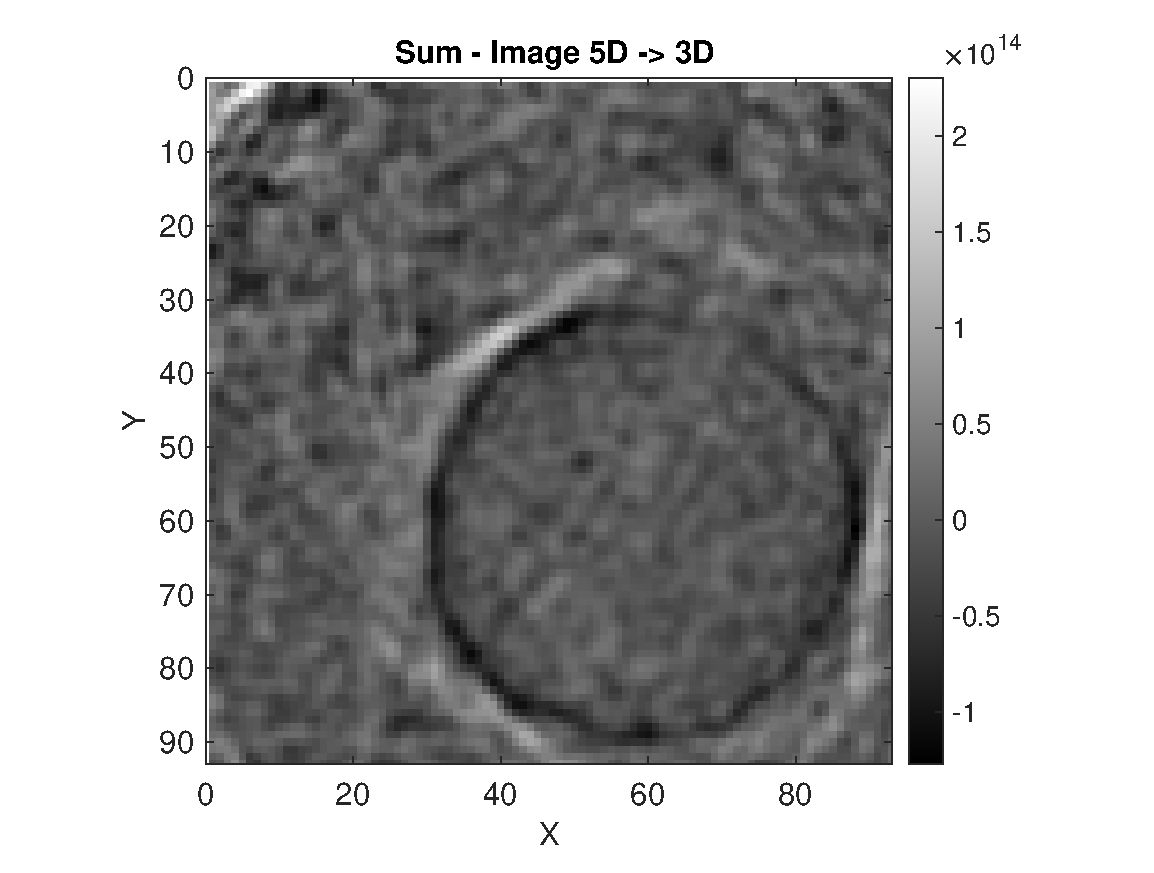
\includegraphics[width=0.69\linewidth]{Graphics/sum_image_35_vec_to_show_that_assign_works.eps}
    \caption{Sum image of the five dimensional data over the 4\textsuperscript{th} and 5\textsuperscript{th} dimension. }
    \label{fig:res:sum_image_35_vec_to_show_that_assign_works}
\end{figure}

The sum image shows the 3D image of the olive and therefore the expected outcome was reached (see for comparison Figure \ref{fig:res:reflec_image_olive_xyz}). If something had gone wrong during the assignment of the directional information, strong visible artefacts would be expected in the sum image that would exceed the expected artefacts of the \ac{saft} image.



\section{Comparison of orthogonality threshold method and angle sorting method}

In section \ref{sec:index_ident} two methods for the assignment of comparison vectors to the right directional vector were explained. It was also mentioned that both methods have different decision regions for the directional vectors. The influence of these differences is shown in this section. In the following all images were created using 25 directional vectors and with the added 4\textsuperscript{th} dimension which stores the information about the voxel-receiver relation. The reason for not also including the 5\textsuperscript{th} dimension was to keep the computation time as small as possible and still being able indicate the differences in the resulting images. Figure \ref{fig:res:slice_diff_bubble_ortho_image} shows a side by side comparison of the reflection image for both assignment methods. From the 4D image the following images are from the 3\textsuperscript{rd} directional vector and the 166\textsuperscript{th} slice in the z-dimension.


\begin{figure}[H]
     \centering
     \begin{subfigure}[b]{0.49\textwidth}
         \centering
        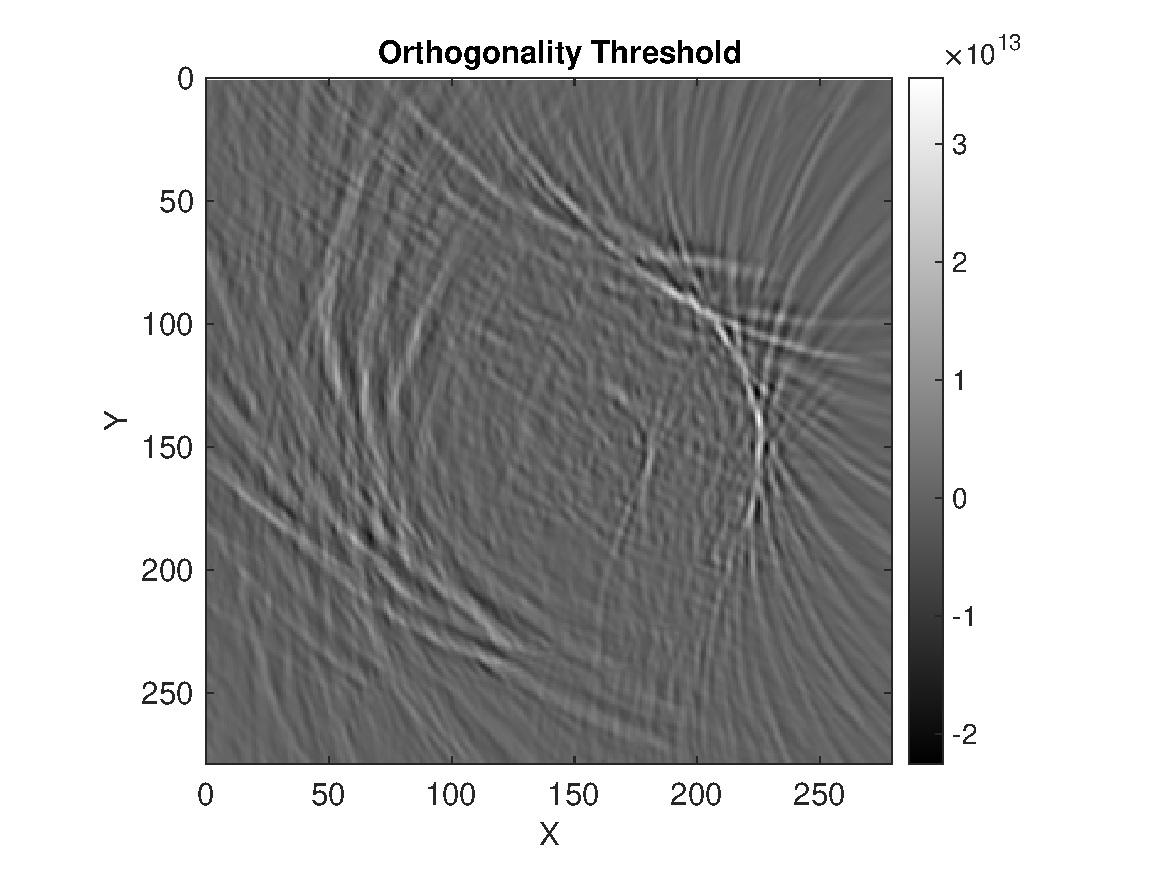
\includegraphics[width=1.12\linewidth,right]{Graphics/Results/Diff_angle_sort_orthogonality/diff_ortho_bubble_slice_166_3_ortho.eps}
         \caption{Orthogonality threshold method.}
         \label{fig:res:slice_diff_bubble_ortho_image_ortho}
     \end{subfigure}
     \hfill
     \begin{subfigure}[b]{0.49\textwidth}
         \centering
         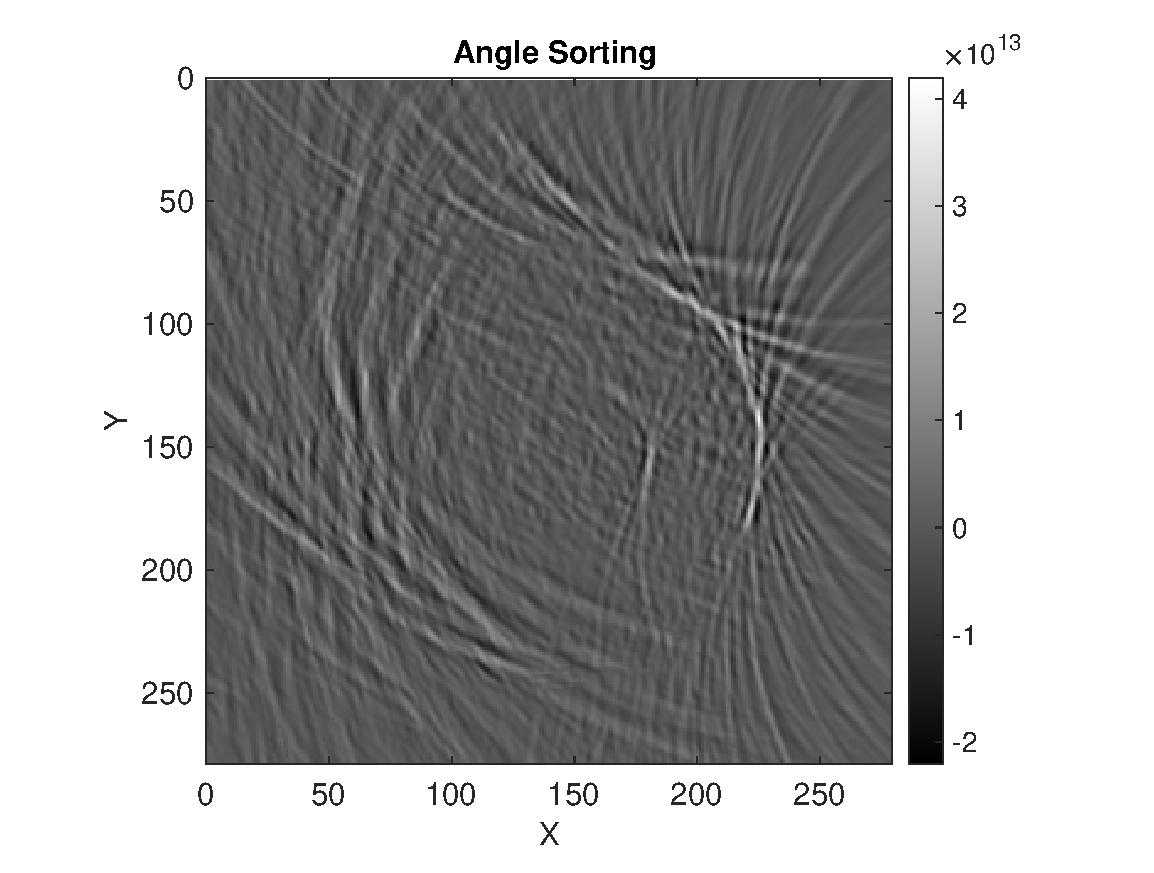
\includegraphics[width=1.12\textwidth,right]{Graphics/Results/Diff_angle_sort_orthogonality/diff_ortho_bubble_slice_166_3_sort.eps}
         \caption{Angle sorting method.}
         \label{fig:res:slice_diff_bubble_ortho_imagebubble}
     \end{subfigure}
        \caption{Side by side comparison of the resulting images for both methods. 25 directional vectors in total were used. The images are shown for the 3\textsuperscript{rd} directional vector and the 166\textsuperscript{th} slice in the z-dimension.}
        \label{fig:res:slice_diff_bubble_ortho_image}
\end{figure}


Figure \ref{fig:res:slice_diff_bubble_ortho_imagebubble} on the right shows a slightly higher contrast than its counterpart on the left. This can be seen in the legend on the right. The highest voxel value for the orthogonality threshold method results in approximately $3.7\times 10^{13}$ where as the amplitude for the angle sorting method is a bit higher at $4.1\times 10^{13}$. The reason for that is that the angle sorting method of section \ref{chap:angle_sorting} assigns every available \ac{ascan} to a directional vector whereas the orthogonality threshold method discards every \ac{ascan} for which the comparison vector lays between the decision cones. 

It has to be remarked that it is not an inherent characteristic of the orthogonality threshold method to discard a certain amount of \acp{ascan}. For this thesis it was implemented in a particular way so that the decision regions of all directional vectors are all are the same size and overlap as little as possible. This implementation leads to as little ambiguity as possible concerning the directional assignment. The non-overlapping decisions regions that are schematically shown in Figure \ref{decision_arbitrary_circular} lead to a consistent quality of the assignment with the same decision criteria for each directional vector. 

For the angle sorting method the decision criteria resulted in different acceptance angles depending on whether the comparison vector points towards a 'tip' of two boundaries of the pentagon or if they were located towards the bisector between two directional vectors. In these cases the quality of the assignment can vary.

\bigskip

In the following image the two methods were compared for one voxel in each of the 25 volumes in the 4\textsuperscript{th} dimension. This representation is generated in a similar manner as the 5D-over-4D representation in Figure \ref{fig:res:5th_dim_over_4th_result} was generated. Since there is no 5\textsuperscript{th} dimension this time only the values for the 4\textsuperscript{th} dimension are plotted. For this representation the analogy of the 4D Rubik's cube array in Figure \ref{4D_rubics} can be taken. Instead of the four Rubik's Cubes we now have 25 and for each of those cubes the voxel value at the the coordinates $[150\, , \, 150\, , \, 166]$ is displayed. For the directional vectors 22 to 25 no or only very few values are shown. The reason for that again is that those directional vectors are pointing out of the aperture and there are no receivers that could detect or emit a signal. 


\begin{figure}[H]
     \centering
     \begin{subfigure}[b]{0.85\textwidth}
         \centering
        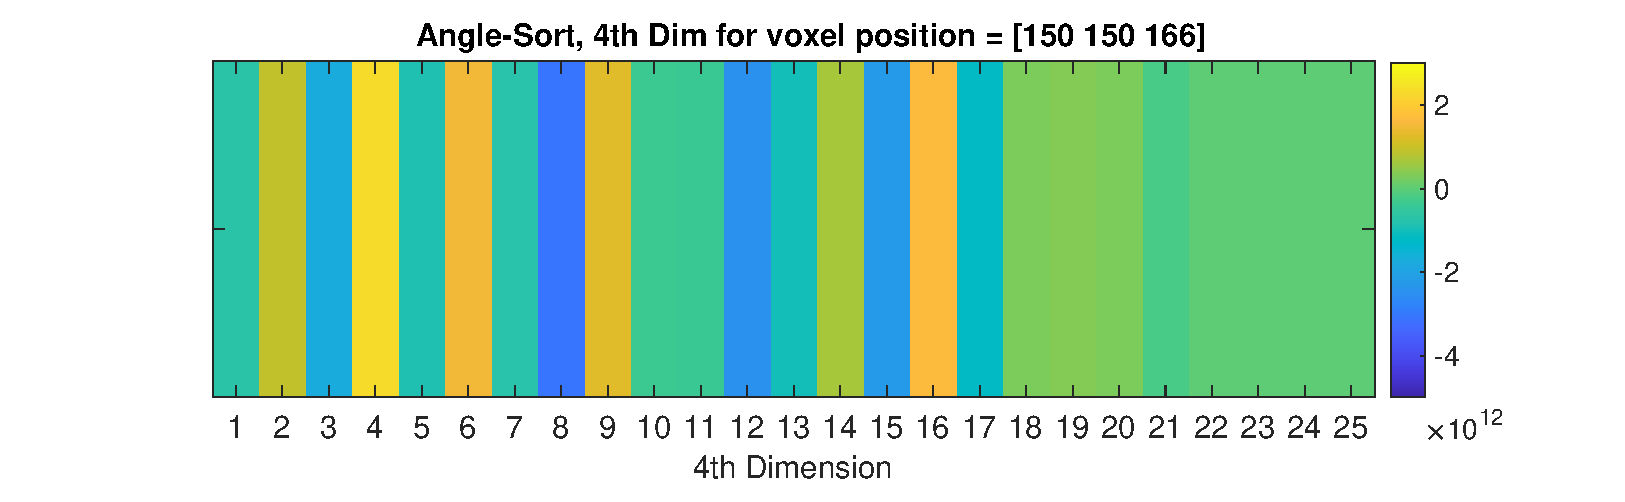
\includegraphics[width=1.12\linewidth,right]{Graphics/Results/Diff_angle_sort_orthogonality/diff_ortho_bubble_25dim_150150150_ortho.eps}
         \caption{Orthogonality threshold method.}
         \label{fig:res:25_voxel_values_diff_bubble_ortho_image_ortho}
     \end{subfigure}
     \hfill
     \begin{subfigure}[b]{0.85\textwidth}
         \centering
         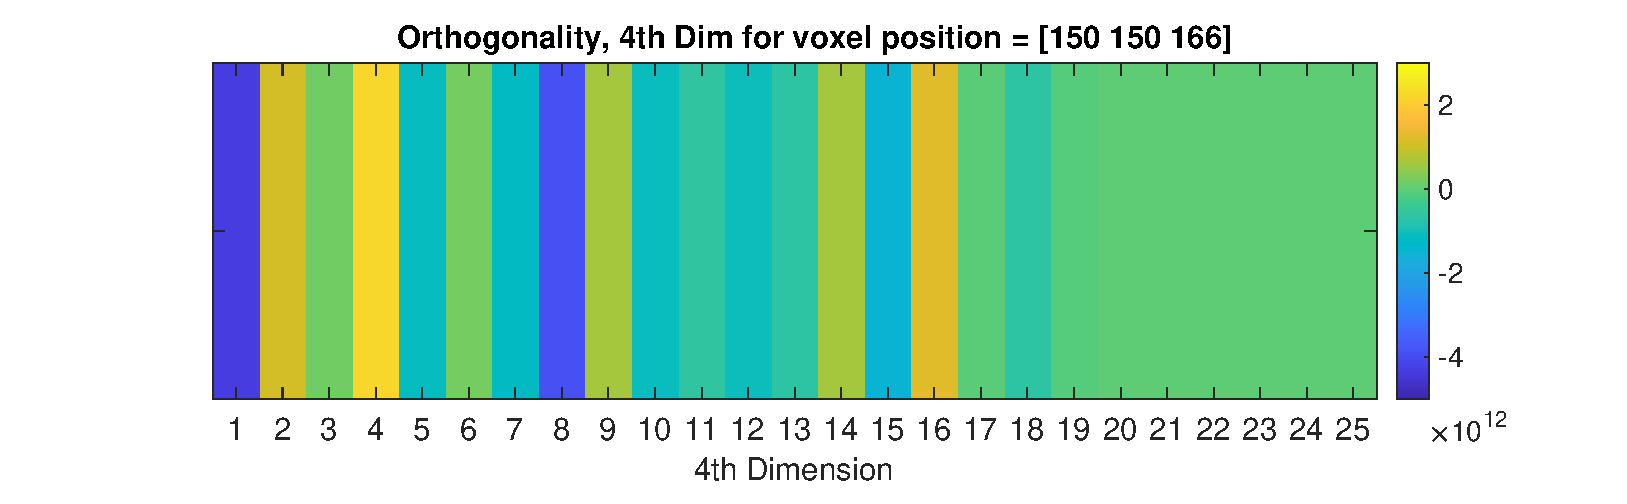
\includegraphics[width=1.12\textwidth,right]{Graphics/Results/Diff_angle_sort_orthogonality/diff_ortho_bubble_25dim_150150150_sort.eps}
         \caption{Angle sorting method.}
         \label{fig:res:25_voxel_values_diff_bubble_ortho_image_bubble}
     \end{subfigure}
        \caption{Comparison of each voxel value for each of the 25 directional vectors.}
        \label{fig:res:25_voxel_values_diff_bubble_ortho_image}
\end{figure}

The overall structure of the array of voxel values for both methods visually appear to be similar. Still, there are some differences e.g. for the 1st directional vector. The voxel value for the orthogonality threshold method was $-4.3171 \times 10^{12}$  where as the voxel value for the angle sorting method was $-7.1738\times10^{11}$. Hence, approximately six times higher than the angle sorting value. For a better comparison of the results shown in figure \ref{fig:res:25_voxel_values_diff_bubble_ortho_image}, in figure \ref{fig:Voxel_value_25} each voxel value for the total of 25 directional vectors is shown in a single plot. The red line shows the voxel values which where yielded by the orthogonality threshold approach. The blue graph belongs to the angle sorting method. In most points the blue line lays above the red line. This corresponds to the assumption that the orthogonality threshold method does not consider every \ac{ascan} and therefore this method yields images with an overall lower voxel values.


\begin{figure}[H]
    \centering
    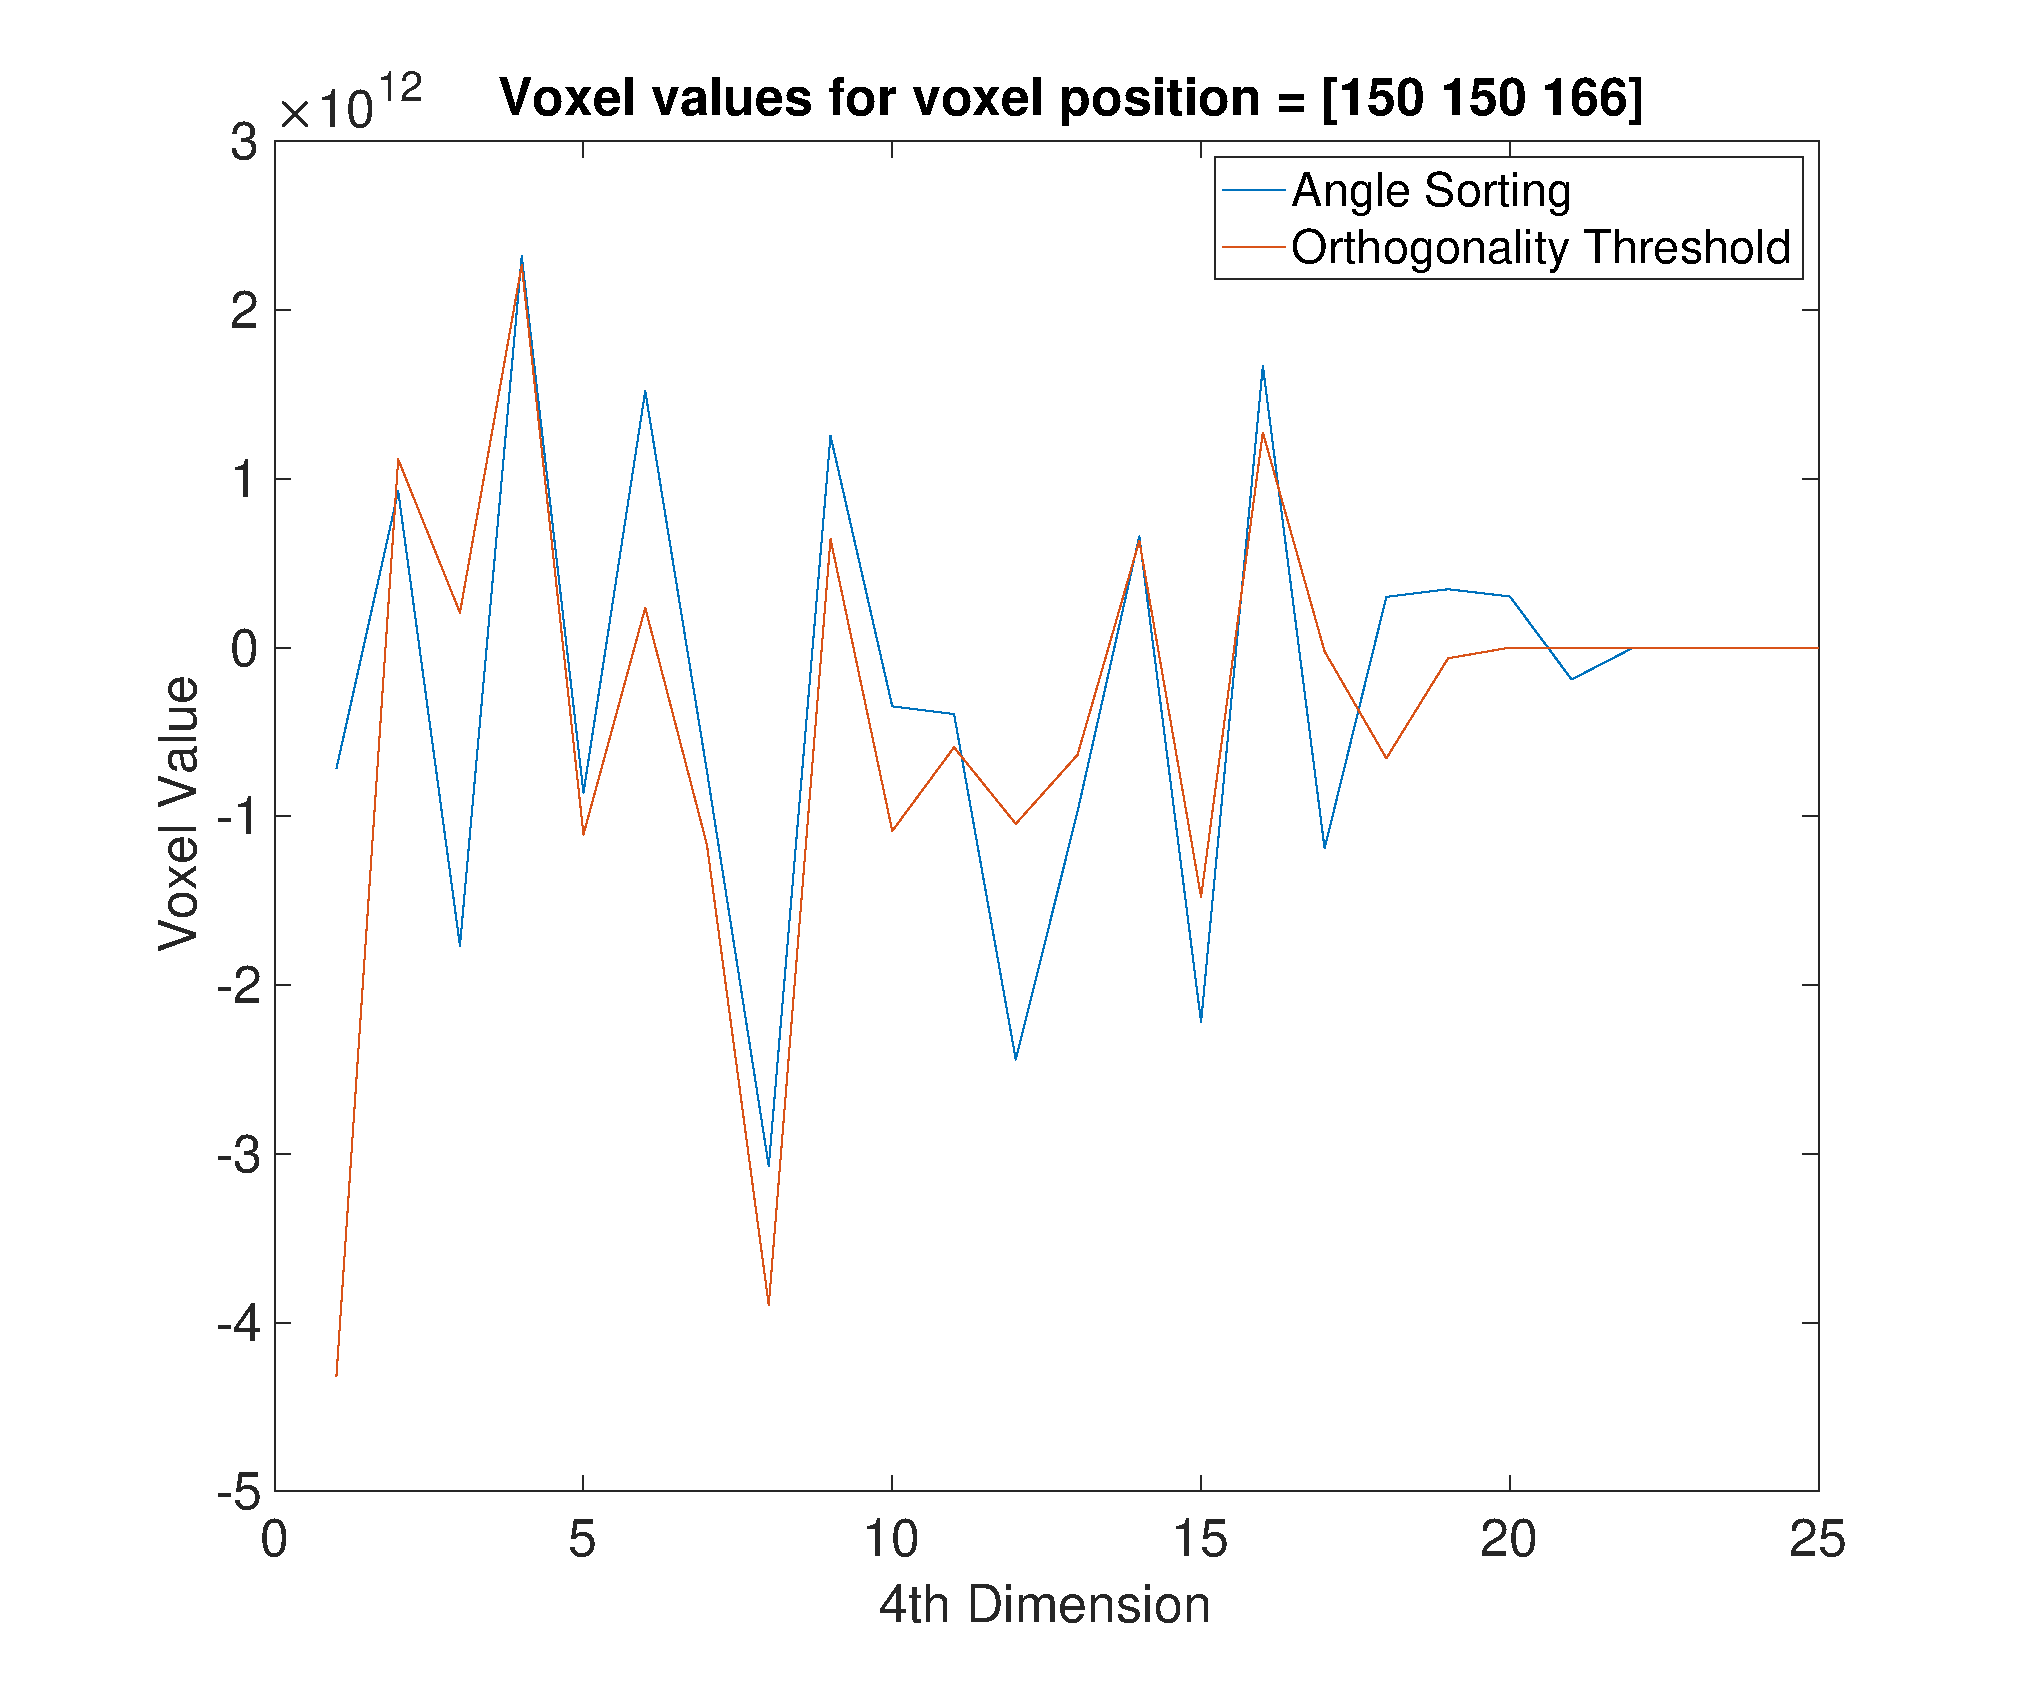
\includegraphics[width=0.82\linewidth]{Graphics/Results/Diff_angle_sort_orthogonality/diff_ortho_bubble_voxelvalues_150150166_sort.eps}
    \caption{Each voxel value of Figure \ref{fig:res:25_voxel_values_diff_bubble_ortho_image} as diagram. The blue graph belongs to the angle sorting Method and the red graph to the orthogonality threshold. }
    \label{fig:Voxel_value_25}
\end{figure}


To make an assessment about how big the influence of the reduced contrast of the Orthogonality Frequency method is the reconstructed 4D images are both reduced to a 3D image. For each of the 25 sub-volumes the same voxel position is considered. This leads to 25 voxel values for one particular voxel in each volume. The mean of those 25 voxel values is calculated and written back into the coordinates of the particular voxel. This is repeated for every voxel there is hence the final images shows approximately the outcome of the standard \ac{saft} without considering the directional information. The final images are shown in figure \ref{fig:res:summareized_bubble_ortho_image}.





\begin{figure}[H]
     \centering
     \begin{subfigure}[b]{0.49\textwidth}
         \centering
         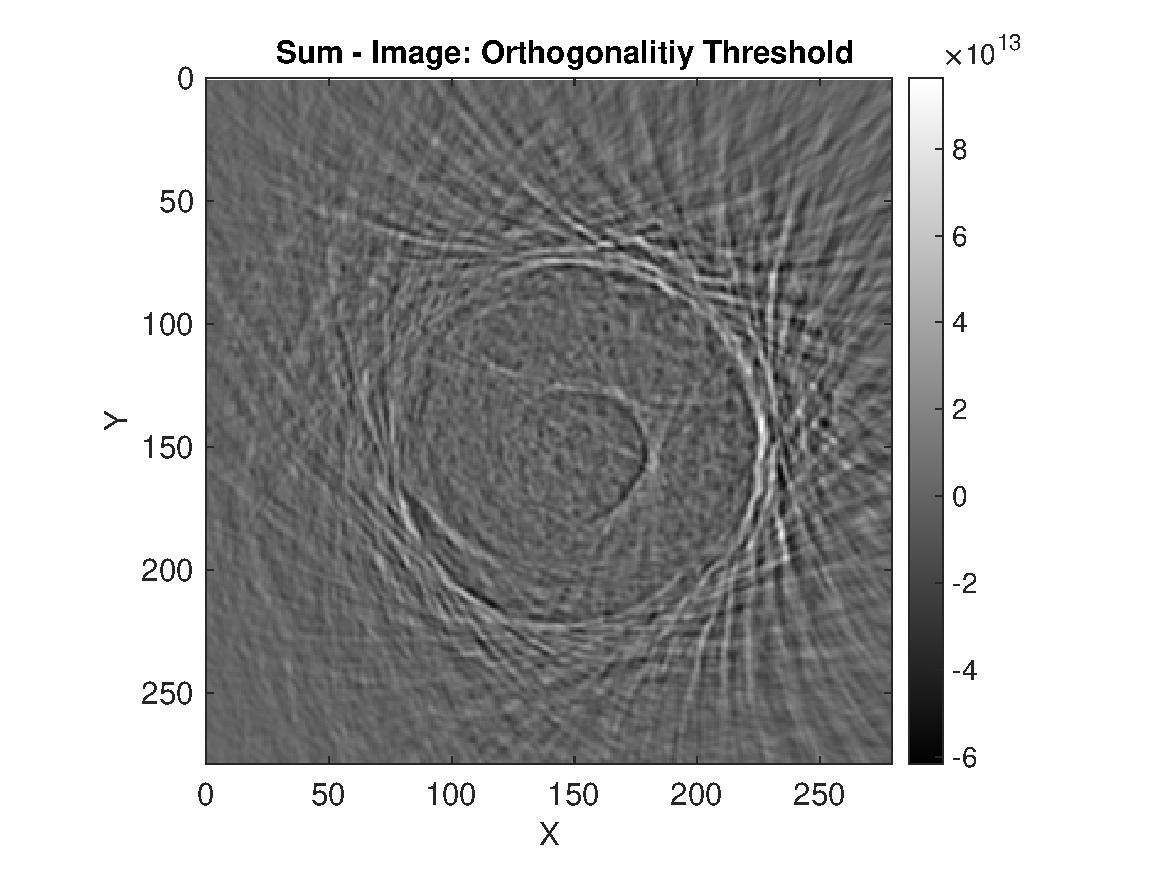
\includegraphics[width=1.12\linewidth]{Graphics/Results/Diff_angle_sort_orthogonality/diff_ortho_bubble_sumImmage_ortho.eps}
         \caption{Orthogonality threshold method.}
         \label{fig:res:summareized_bubble_ortho_image_ortho}
     \end{subfigure}
     \hfill
     \begin{subfigure}[b]{0.49\textwidth}
         \centering
         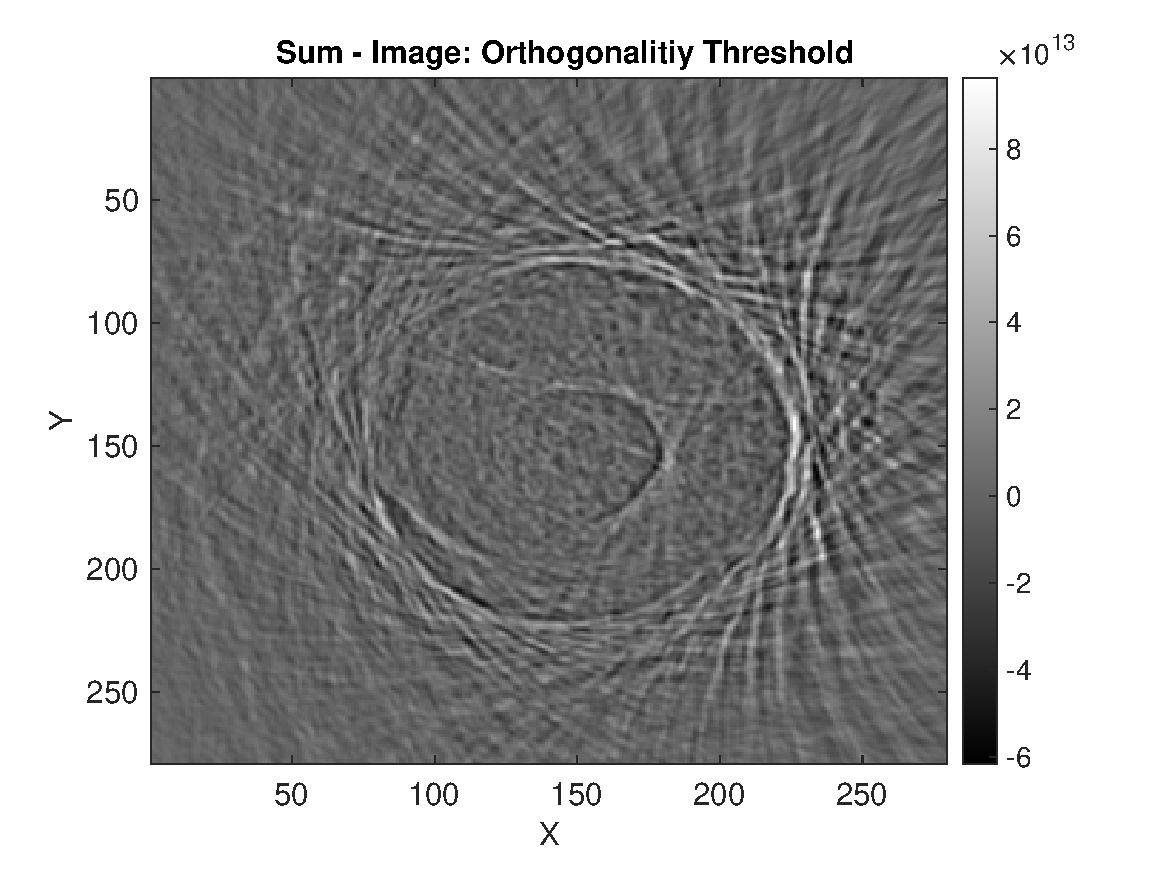
\includegraphics[width=1.12\textwidth]{Graphics/Results/Diff_angle_sort_orthogonality/diff_ortho_bubble_sumImmage_sort.eps}
         \caption{Angle Sorting method.}
         \label{fig:res:summareized_bubble_ortho_image_bubble}
     \end{subfigure}
        \caption{Summarised image where the 4D image was reduced to a 3D image. }
        \label{fig:res:summareized_bubble_ortho_image}
\end{figure}

Again the 166\textsuperscript{th} slice in the z-direction is shown. In comparison to Figure \ref{fig:res:slice_diff_bubble_ortho_image} the olive in the middle of the volume becomes much more prominent since reflections from all directions are considered. In the image of only one directional vector the olive in Figure \ref{fig:res:slice_diff_bubble_ortho_imagebubble} showed a high intensity of sound waves in the top right corner of the olive. The outline of the gelatin block around the olive becomes more prominent as well. With the summation of all the images the directional information is lost however. Both images in figure \ref{fig:res:summareized_bubble_ortho_image} contain enough detail to make out the gelatin block with the olive in the middle. A difference concerning the noise level can not be observed. Again the angle sorting method results in a higher amplitude compared to the orthogonality threshold. The orthogonality threshold has a maximum voxel value of approximately $9 \times 10^{13}$ whereas the amplitude of the solution of the angle sorting method in Figure \ref{fig:res:summareized_bubble_ortho_image_bubble} reaches $8.7 \times 10^{13}$. 

A qualitative representation of the differences between both sum images is given in Figure \ref{fig:diff_image}.

\begin{figure}[H]
    \centering
    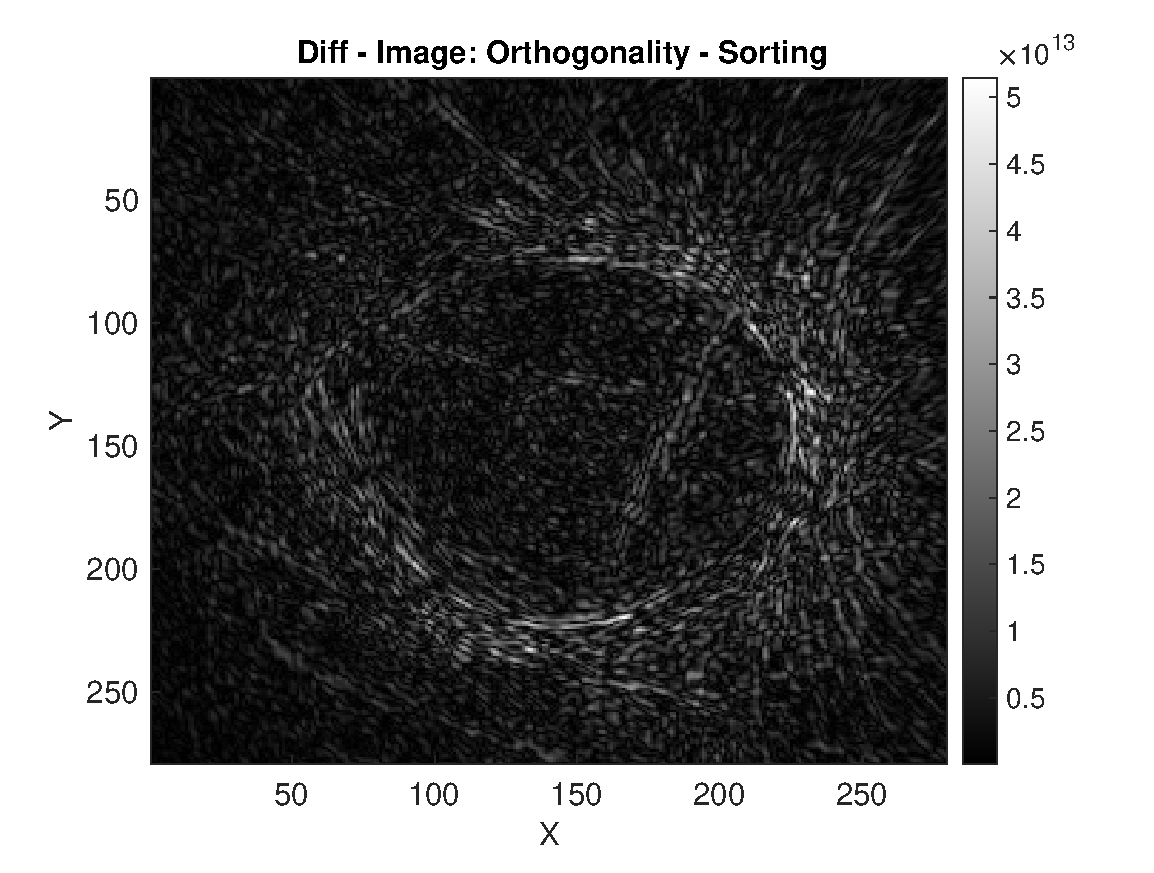
\includegraphics[width=0.82\linewidth]{Graphics/Results/Diff_angle_sort_orthogonality/diff_ortho_bubble_diffimage.eps}
    \caption{Absolute value of the difference between the summarised image of the Orthogonality Method and the Angle Sorting method. }
    \label{fig:diff_image}
\end{figure}

The difference image shows that the inside of the gelatin block and the olive is mostly unaffected by the new approach. Big differences can only be observed on the outer boundary of the gelatin block. The olive can not be distinguished in the difference image. Therefore, the new methods does not influence that part of the image which is a desirable result. The new approach leads to a different amplitude in the reconstructed images compared to angle sorting approach. However, the part of the image that contains valuable information is not influenced at all. 



\section{Performance of the directional dimension assignment methods}
\label{performance_index_ident}

In Section \ref{sec:index_ident} two main approaches were presented for the assignment of the directional vector index to each \ac{ascan}. In this chapter the results of the performance evaluation of the angle sorting approach from section \ref{chap:angle_sorting} and the threshold orthogonality from section \ref{chap:ortho_threshold} are shown. 

For the performance analysis the general structure of the reconstruction from Figure \ref{Basic_Algo_Angle_ident} is adapted. To speed up the process, the 5\textsuperscript{th} dimension is kept constant during the execution. This leads to a four dimensional image instead of a five dimensional. For the evaluation a script was written which calls the reconstruction function with an increasing amount of directional vectors. For each choice of the number of directional vectors the four dimensional image is reconstructed in whole. The procedure is repeated for the angle sorting approach and the new orthogonality approach separately.

The following calculations were performed on two \acp{gpu} (NVidia GeForce 2080 Ti) with a reconstruction volume of $279\times279\times233$ voxels. Furthermore, the block of 30235 \acp{ascan} were used during the reconstruction to speed up the process. The four dimensional case was considered and therefore only the comparison vector from the voxel to the receiver was used. No results besides the profiling report were saved to minimise the influence of hard drive operations during the performance evaluation. The execution time includes all initialisation steps of the reconstruction algorithm as well as generation of directional vectors. The calculation of the threshold orthogonality (in case of the application of the orthogonality threshold method) is also considered by these results. The first reconstruction was started for 14 directional vectors and the last ended at 126. The current implementation allows to generate and arbitrary set of directional vectors starting at 14. Sets with fewer directional vectors than 14 were generated with the platonic solid approach. For the performance evaluation it was necessary to increase the number of directional vectors arbitrarily and the evaluation starts with 14 input vectors.

The following three figures shows the comparison of the computation time of the different techniques for the index identification introduced in section \ref{sec:index_ident}. The results for the sorting algorithm are presented in blue where as the approach with the orthogonality threshold is shown in red.

\begin{figure}[H]
    \centering
    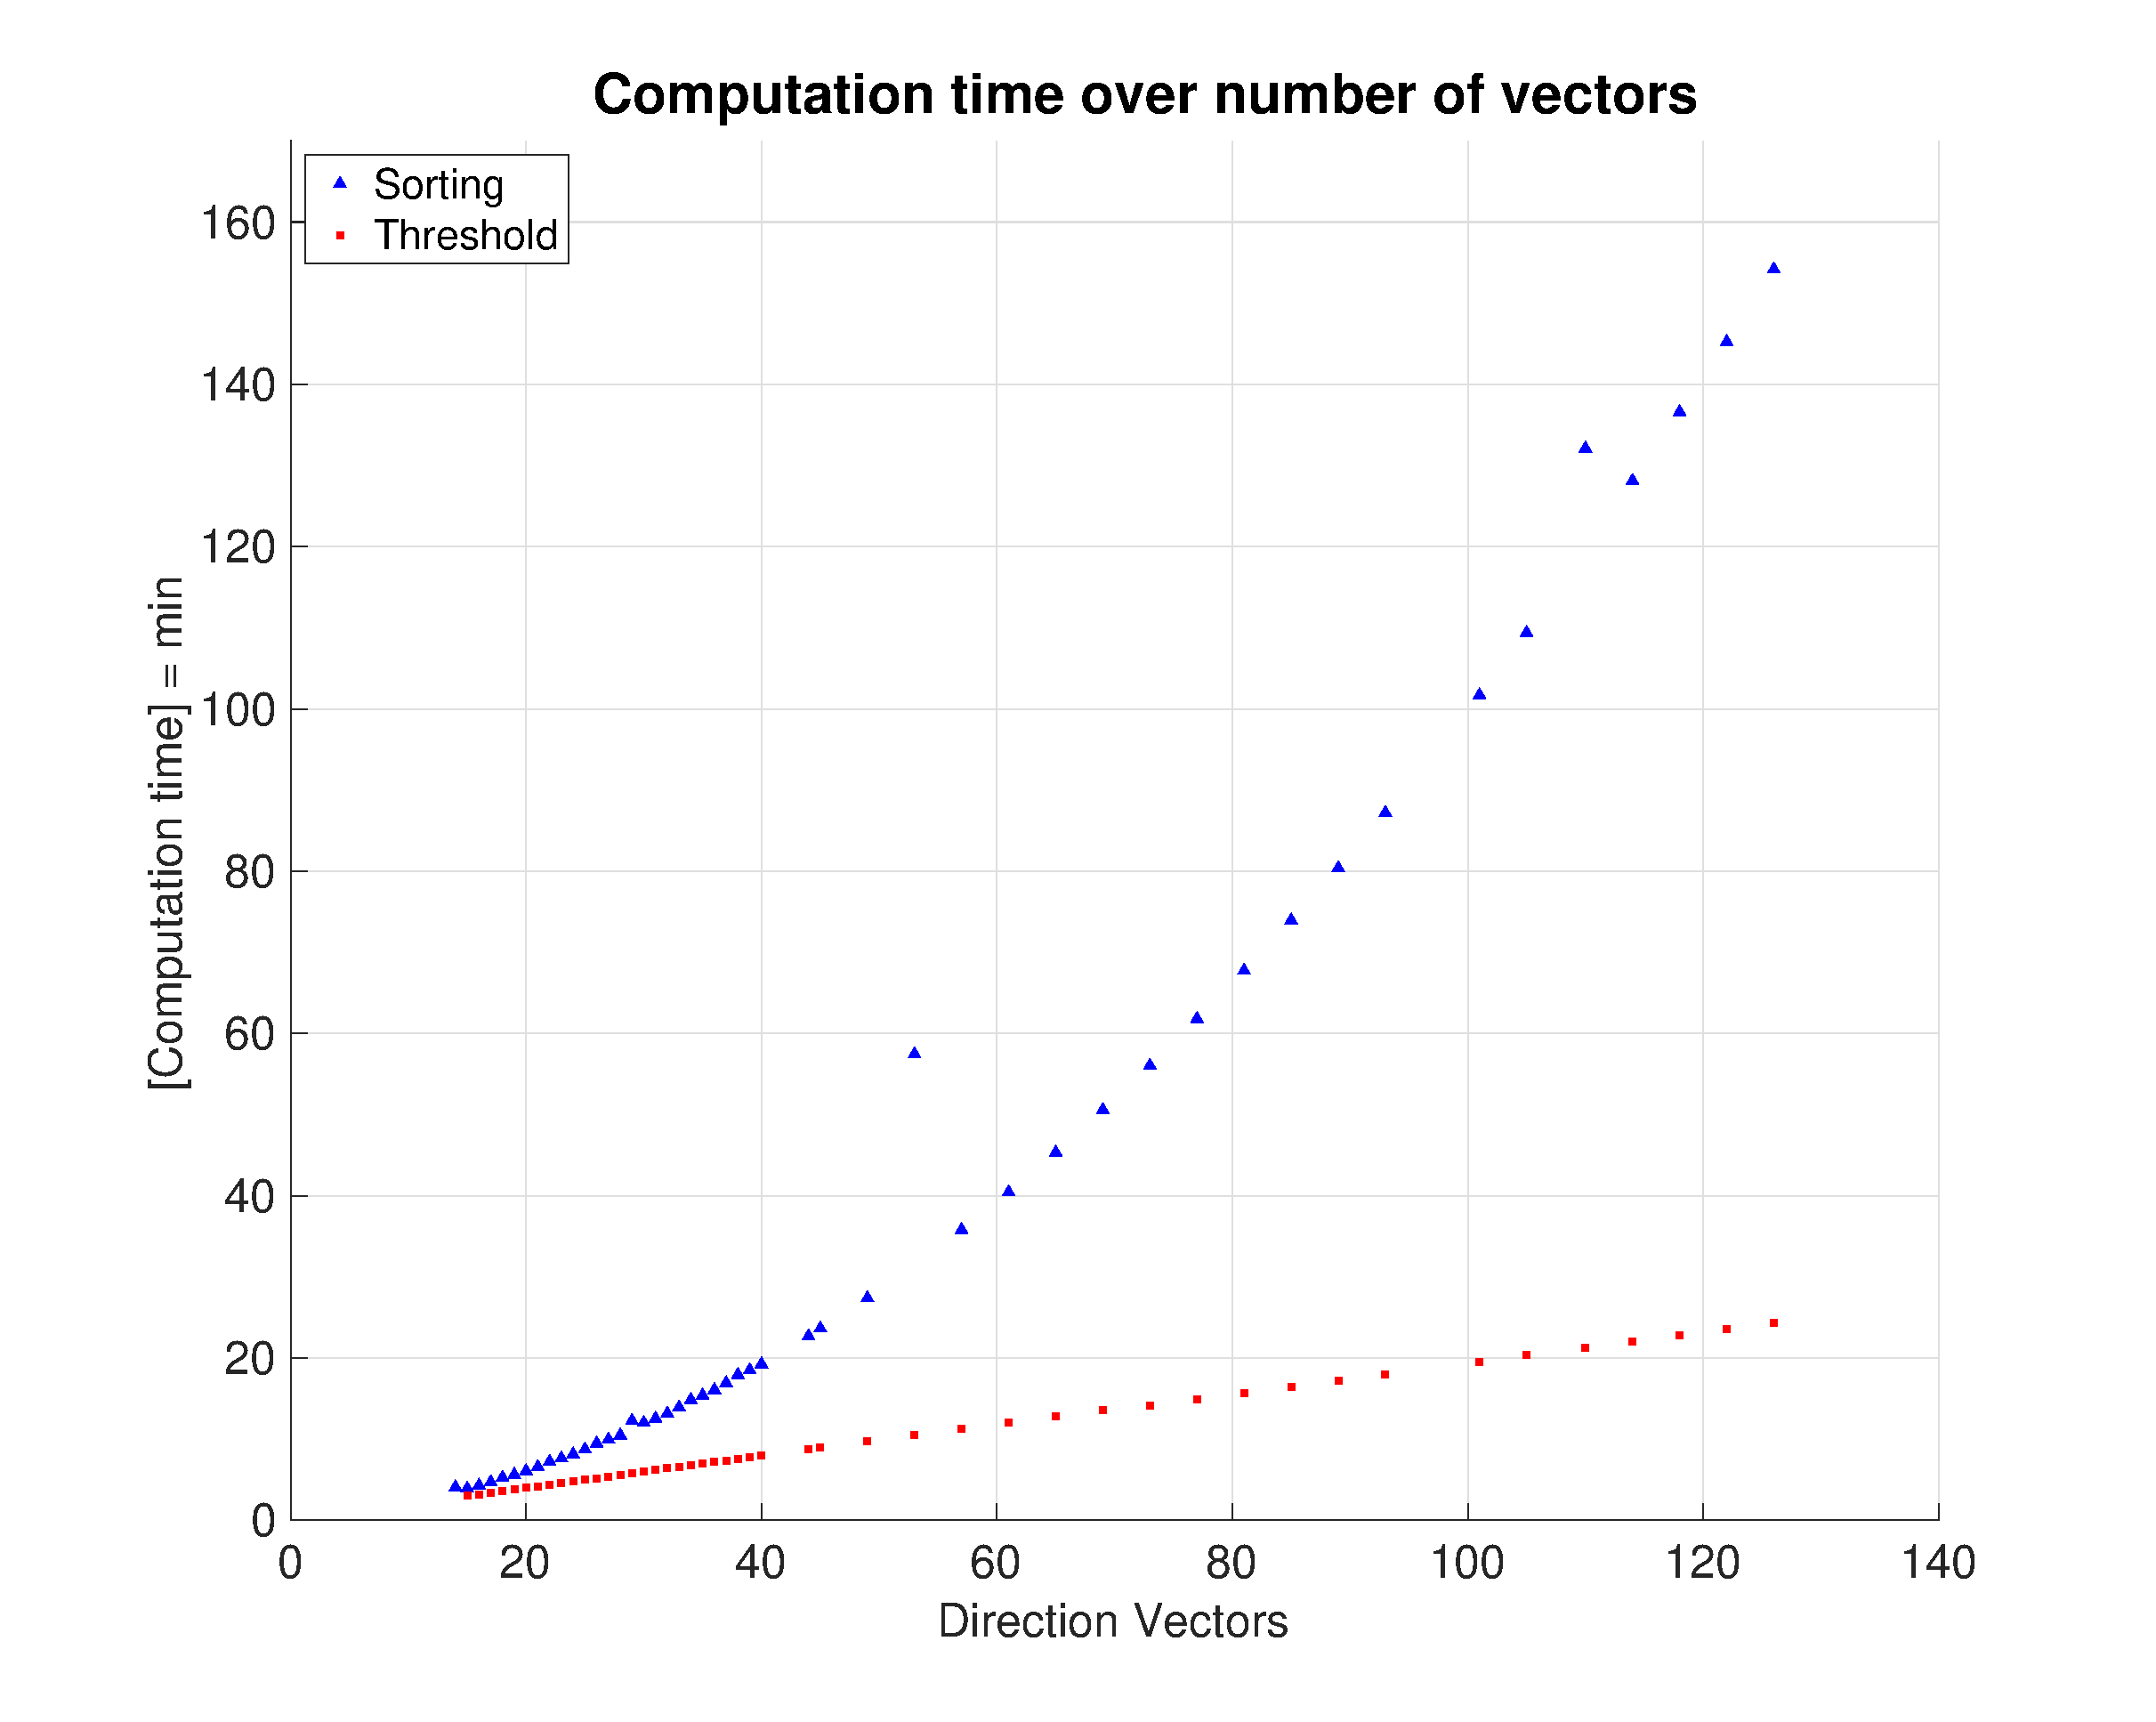
\includegraphics[width=1\linewidth]{Graphics/Results/complete_computation_time_over_numer_vec.eps}
    \caption{Total time of computation given in minutes for 30325 \acp{ascan} and for all loops over the directional vectors. The red markers represent the execution time for the orthogonality threshold method. The blue markers belong to the angle sorting algorithm.}
    \label{fig:Complete_computation_all_vecs}
\end{figure}

The blue triangle markers in Figure \ref{fig:Complete_computation_all_vecs} represent the execution time for the angle sorting algorithm. The horizontal distances between the succeeding markers is associated with the attempt to decrease the overall length of the experiment. For shorter execution times (up to 20 minutes per call) for both algorithms the amount of directional vectors were increased one by one after each iteration. The following steps were increased by four input vectors per iteration.

For a small number of directional vectors the execution time of the angle sorting algorithm and the orthogonality threshold are relatively close, both taking approximately three minutes to compute. With increasing number of directional vectors the application of the angle sorting algorithm leads to a longer sorting loop. This can be seen in the exponential growth of the execution time for the implementation of the angle sorting method. In contrast the implementation of the orthogonality threshold method shows a linear behaviour when the number of directional vectors is increased. For the final 126 directional vectors the sorting algorithm takes $154 \min$ whereas the orthogonality method takes $24.3 \min$ to finish, thus being $10.5$ times higher than the faster orthogonality method. For 45 directional vectors the reconstruction with the angle sorting method takes $23.6 \min$ and thus approximately as long as the orthogonality method takes with 126 directional vectors.

The execution times of each iteration and number of directional vectors include a significant amount of overhead, as it was mentioned further above. Since the overhead is expected to be constant for every execution of the reconstruction algorithm. Regardless of the overhead these results still show the considerable influence of the assigning algorithm on the overall performance.

During the performance evaluation certain iterations took an unusual amount of time to finish and led to some outliers in the computation time for the sorting algorithm. Those were non-reproducible for the particular number of directional vectors for when they occurred but were kept in the graph for reasons of consistency. One possible explanation might be the accidental use of the same  \acp{gpu} by another process or other occurrences that might have led to the simultaneous occupation of servers resource and thus a decreased performance of the reconstruction algorithm since multiple people have access to it. This should be investigated in the future.


\begin{figure}[H]
    \centering
    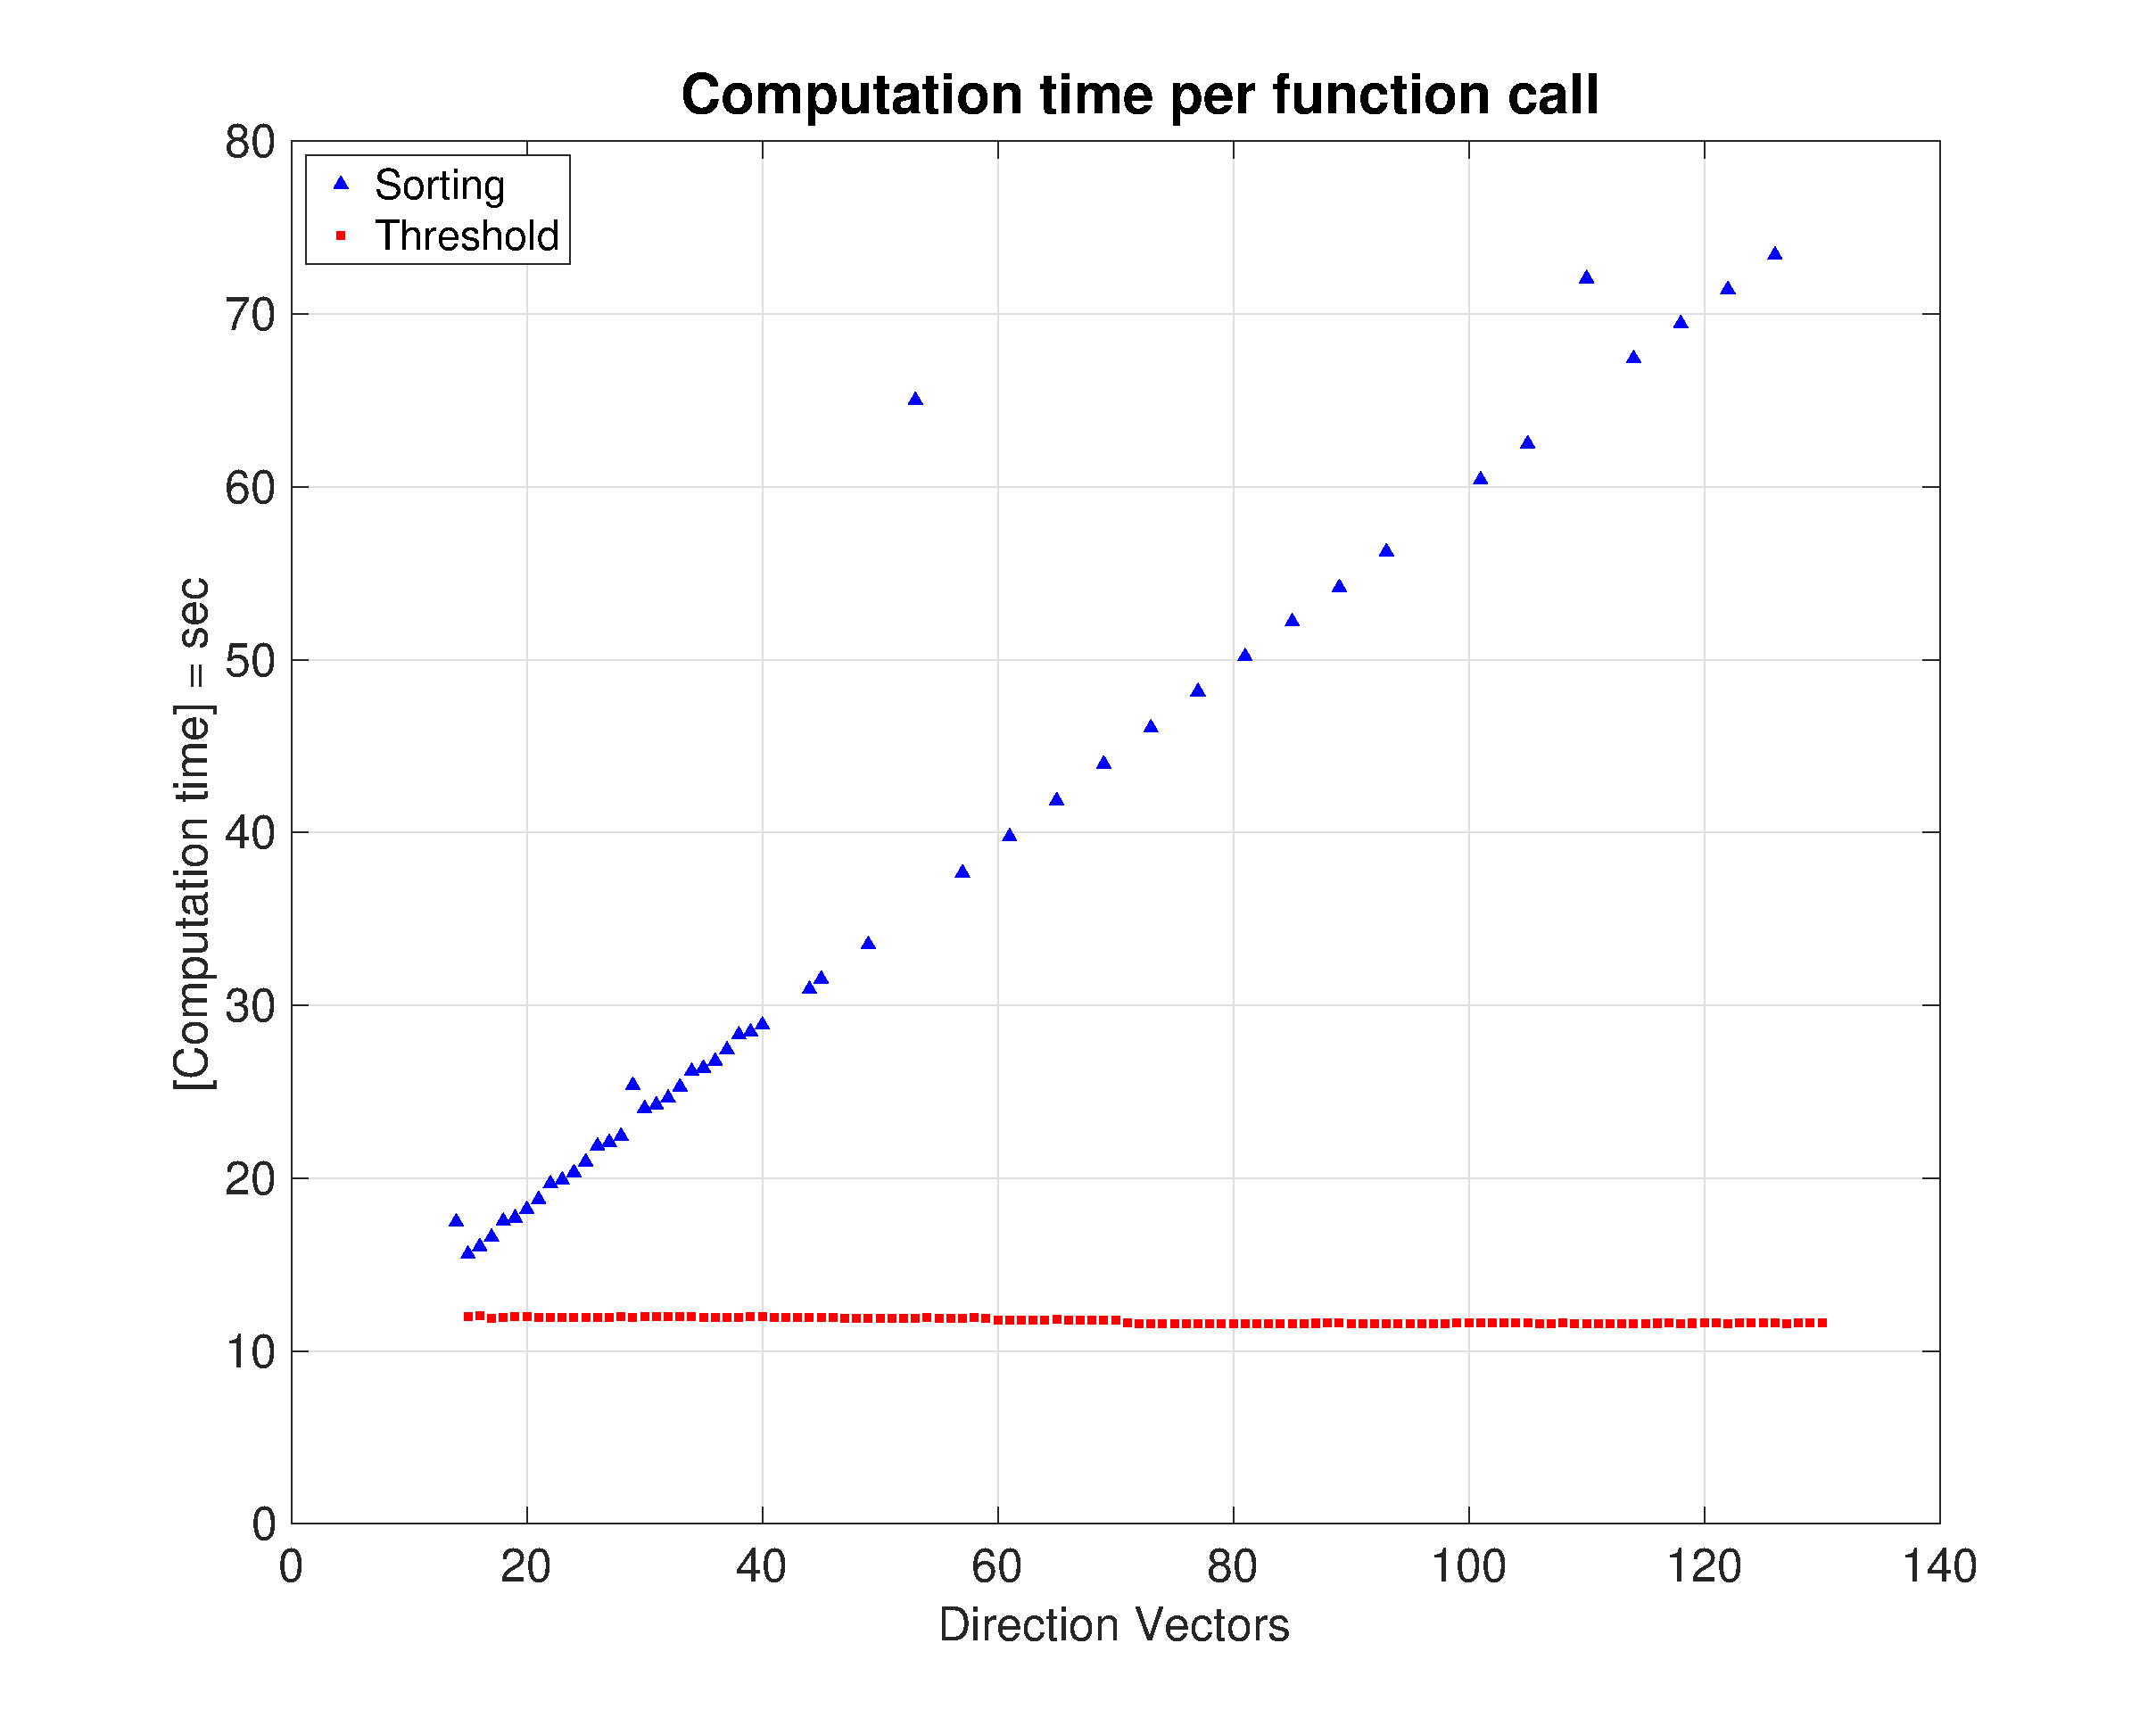
\includegraphics[width=1.08\textwidth]{Graphics/Results/computation_time_per_mexcall.eps}
    \caption{The computation time of each individual function call in $\sec$. The execution time was divided by the number of input vectors to quantify the performance for one function call.}
    \label{fig:computation_per_mex}
\end{figure}

In Figure \ref{fig:computation_per_mex} the execution time for only one iteration of the reconstruction is shown. The complete computation time was divided by the number of input directional vectors to approximate the execution duration for only one function call. The resulting plot shows that the execution time for the orthogonality threshold method is rather constant for an increasing number of directional vectors. In contrast the execution time for each function call with the implementation of the sorting algorithm takes an increasing amount of time to finish. The outliers in the set of blue markers are visible again in this plot. The red markers for the threshold method seem to have a step at about 70 input vectors. The reason for that most likely is the different time of day when the executions were started. They were not done consecutively but sometimes had to be restarted at a later point. This also was the case for the performance analysis for the threshold method. Beginning with 70 input directional vectors the profiling script was restarted the day after. The reason for the small difference in execution time again might be found in the shared resources on the server and the non-constant load during the calculations. 



\begin{figure}[H]
    \centering
    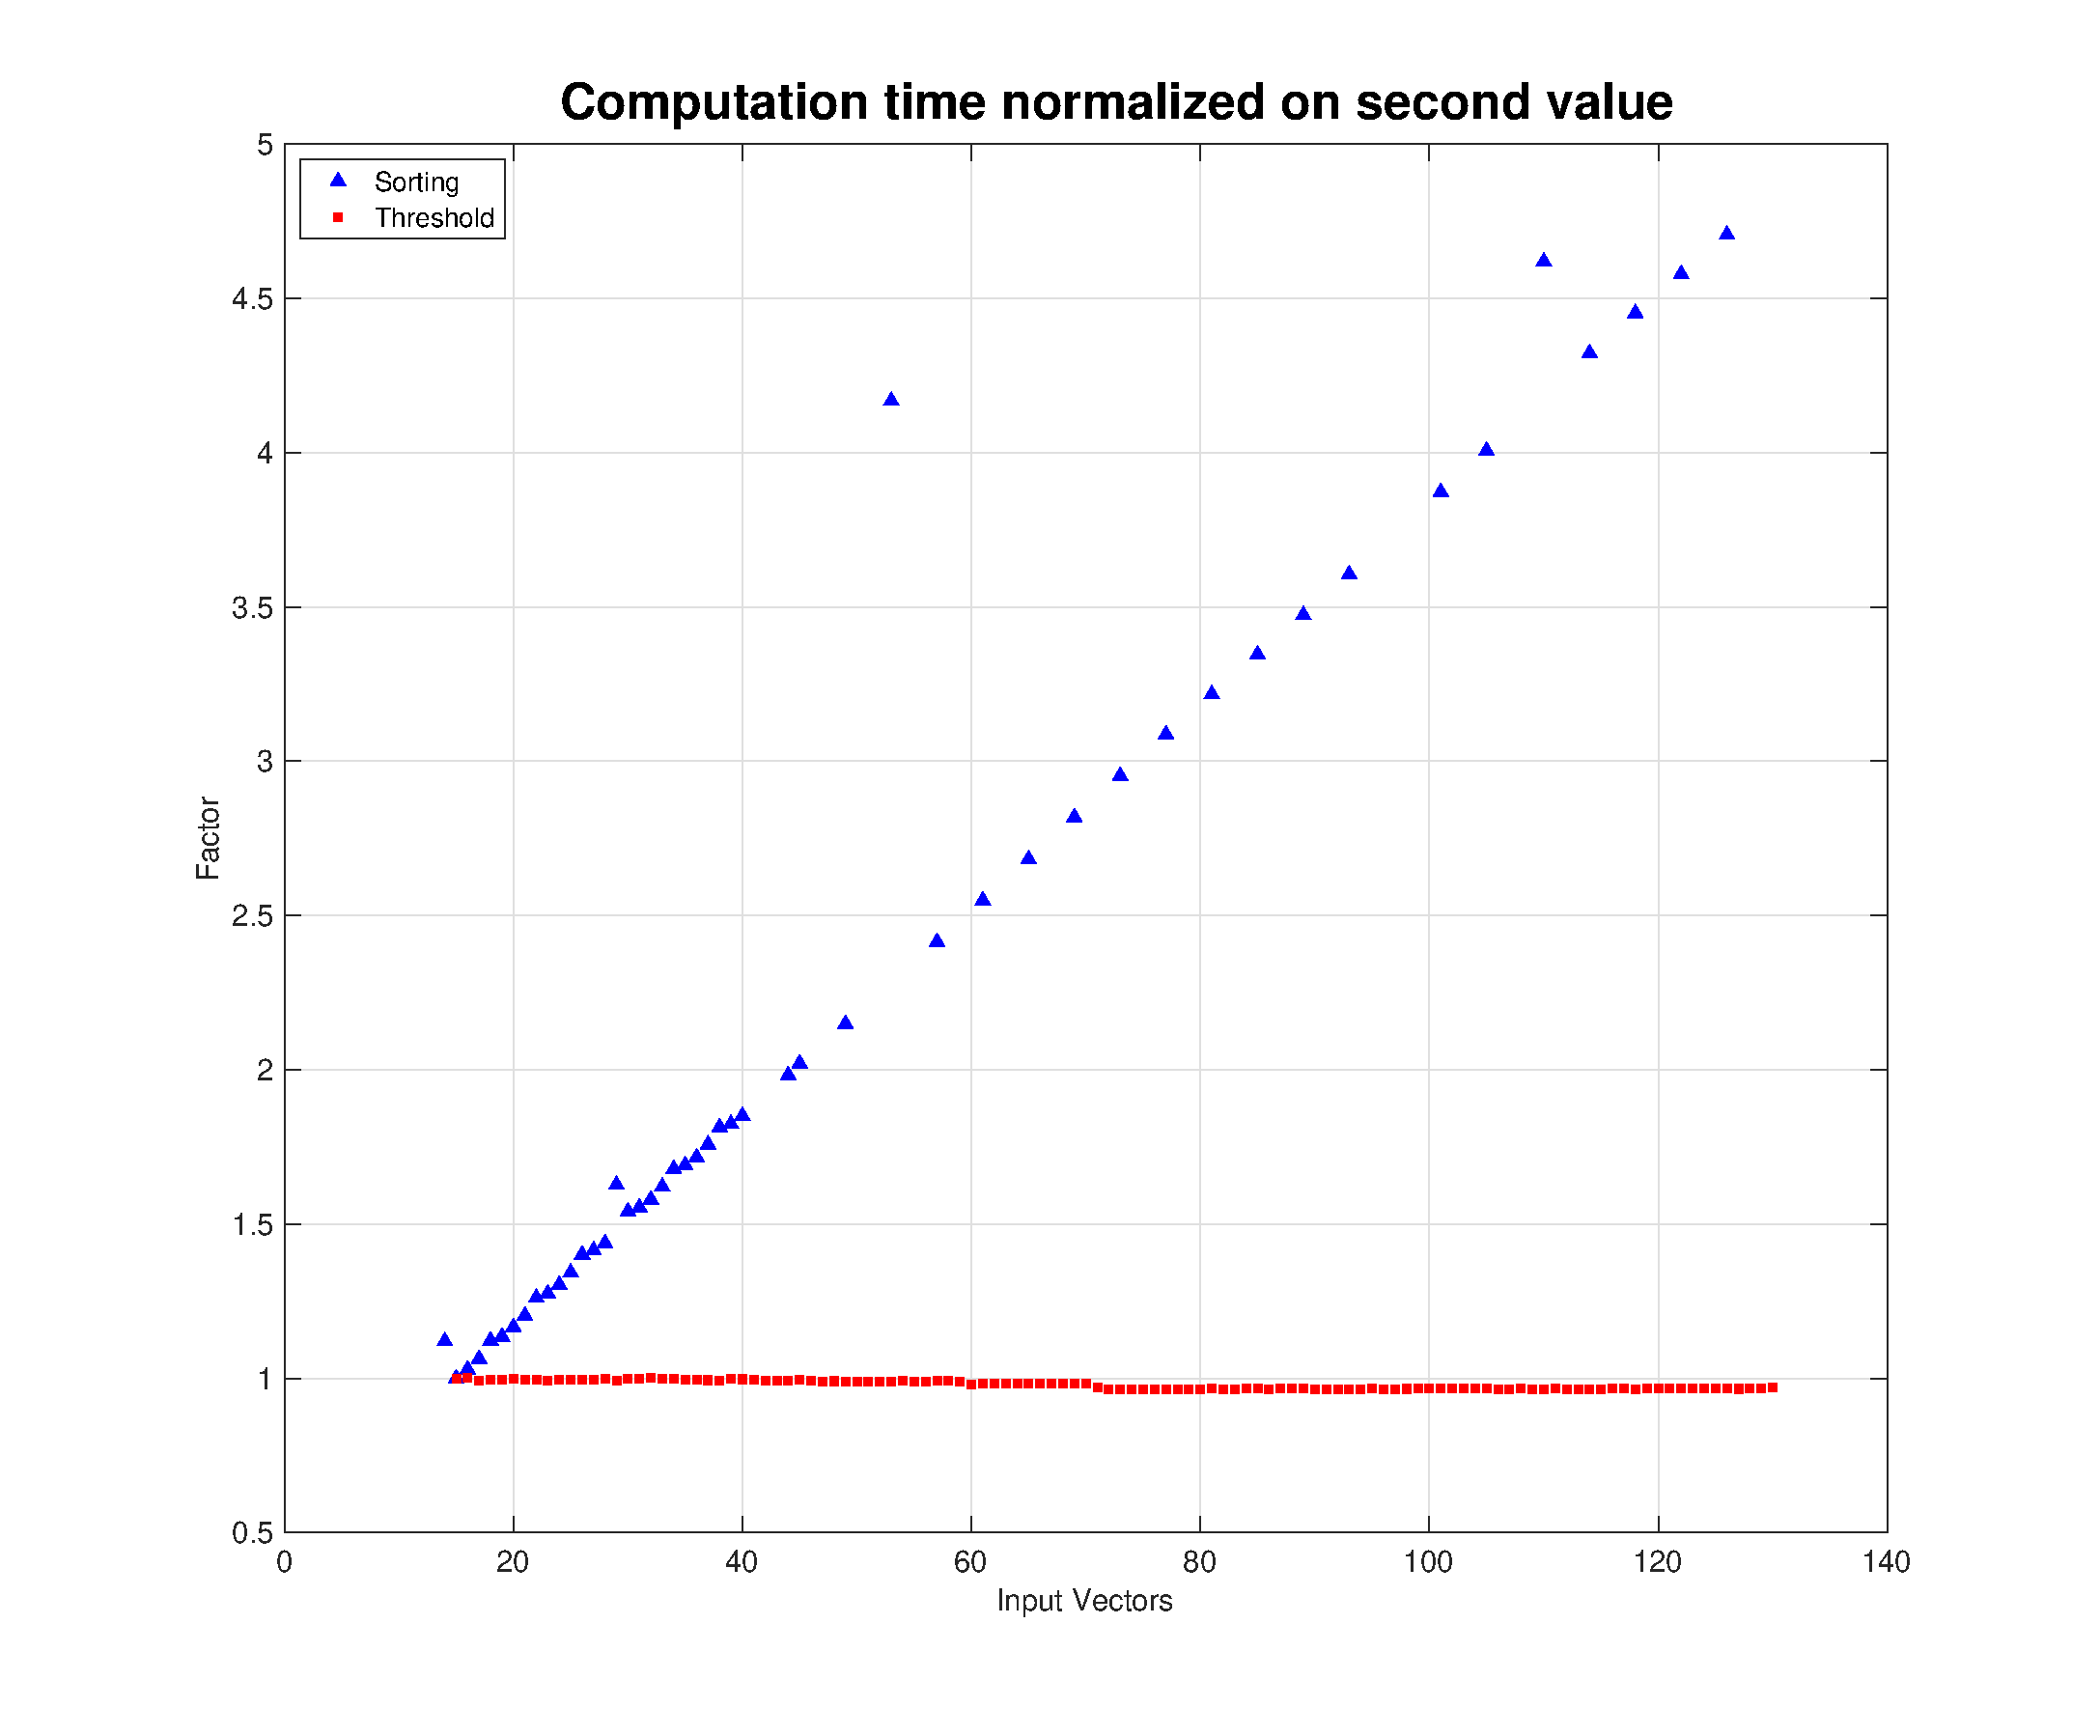
\includegraphics[width=1.08\textwidth]{Graphics/Results/computation_normlaized_2nd_value.eps}
    \caption{The computation time of each individual function call was normalised on the 2nd value of both methods.}
    \label{fig:computation_normlaized_2nd}
\end{figure}

To quantify the differences in performance between both approaches in Figure \ref{fig:computation_normlaized_2nd} the execution times for both methods were normalised on their respective second value. The second value was preferred over the first one since the first iteration always took a bit longer than the following one. A reason for that might be initial behaviour of the servers processing unit  e.g. the optimisation of the cache management at the beginning of the calculations. Nevertheless, in both cases the markers for 14 directional vectors begin at the factor 1 and increase over the following iterations with more input vectors. At least this is the case for the angle sorting method. The markers for the orthogonality threshold stay rather constant at 1 whereas the blue markers end up at a factor of $4.706$ for 126 input vectors. Here again the small step around the 70 input vectors arise from the different times of the start of the analysis.





\section{Evaluation of the differentiation of tissue by directional information}
\label{sec:res:eval_diff_tissue_type}


The following results all were created with the orthogonality threshold method from section \ref{chap:ortho_threshold} since this method has proven to be much more computationally efficient (see section \ref{performance_index_ident}) as well as to yield an approximation of the results from the angle search method. The volume was restricted to minimise the computation time and Figure \ref{fig:res:reflec_image_olive_xyz} shows the location of the reconstructed volume. For these results 35 directional vectors were created with the arbitrary segmentation approach. Per \ac{tas} one sender and nine receivers were selected. To reduce the computation time only four of the ten available aperture positions were included. The data set from the setup in section \ref{sec:input_data} was used. Data of a simple setup of one small test object was preferred over complex clinical data. As a next step this procedure could be tested on simulated data where a ground truth about reflection properties of different test objects were known. 



In section \ref{fig:res:5th_dim_over_4th_result} the 5D-over-4D-representation of different voxels inside of the 5D data was introduced. This representation will now be used to analyse the characteristics of different tissue types (i.e. materials of the olive and the gelatin). The 5D-over-4D-representations for the three different test voxels is plotted in Figure \ref{fig:res:5D_4D_skin_pulp_compare}. 

In this image we see all the 4D-5D voxel values for the reconstructed data. As a reminder: the 5\textsuperscript{th} dimension comprises directional information for the direction from the voxel to the emitters whereas the 4\textsuperscript{th} dimension contains the information for the voxel to the receiver direction. With that in mind it becomes clear that the directional vectors $30, 31, 32, 33, 34$ and $35$ are pointing out of the imaging aperture and neither any emitter nor any receiver is located in this direction. Therefore, neither of the three 5D-4D-representation does hold any directional information for those directional vectors.

\begin{figure}[H]
     \centering
     \begin{subfigure}[b]{0.47\textwidth}
         \centering
        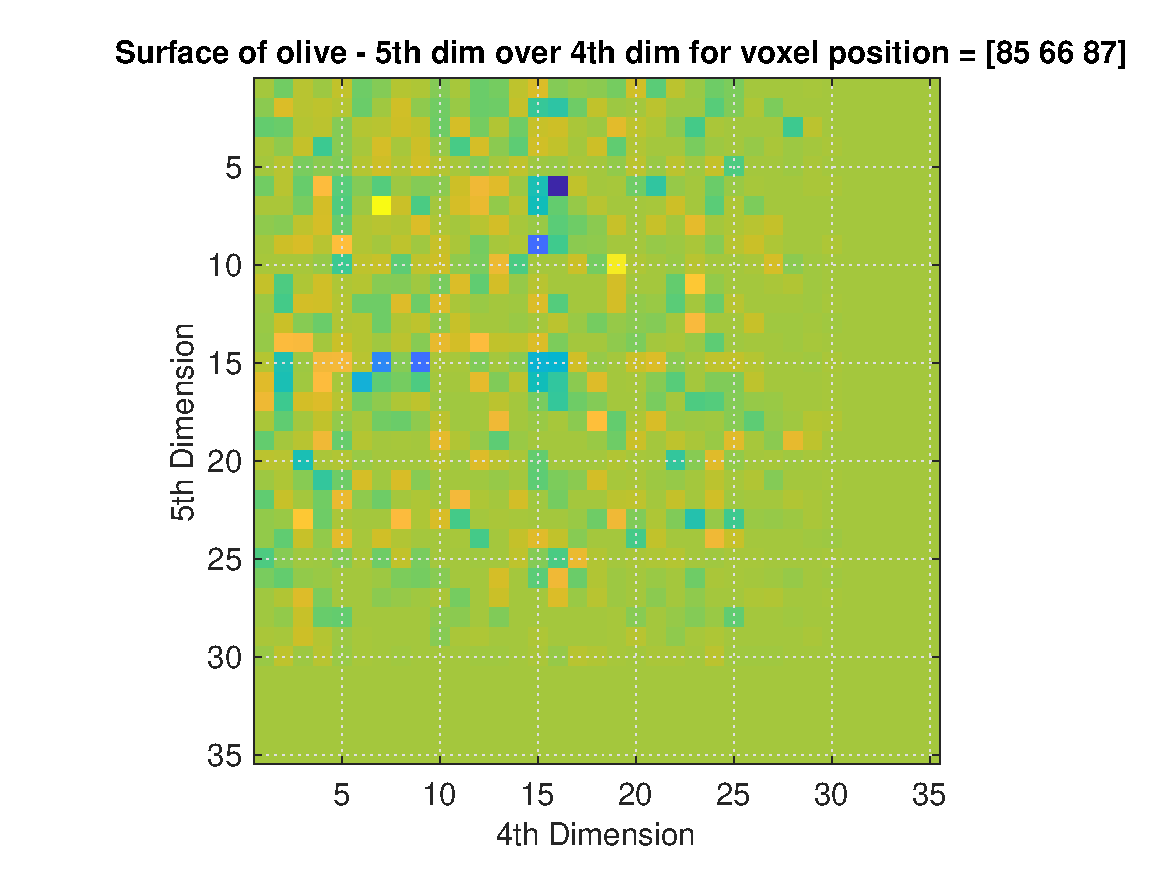
\includegraphics[width=1.09\linewidth]{Graphics/Results/skin_pulp_stone_5D_4D_Stone.eps}
         \caption{Surface of olive. }
         \label{fig:res:5D_4D_skin_pulp_compare_stone}
     \end{subfigure}
     \hfill
     \begin{subfigure}[b]{0.47\textwidth}
         \centering
         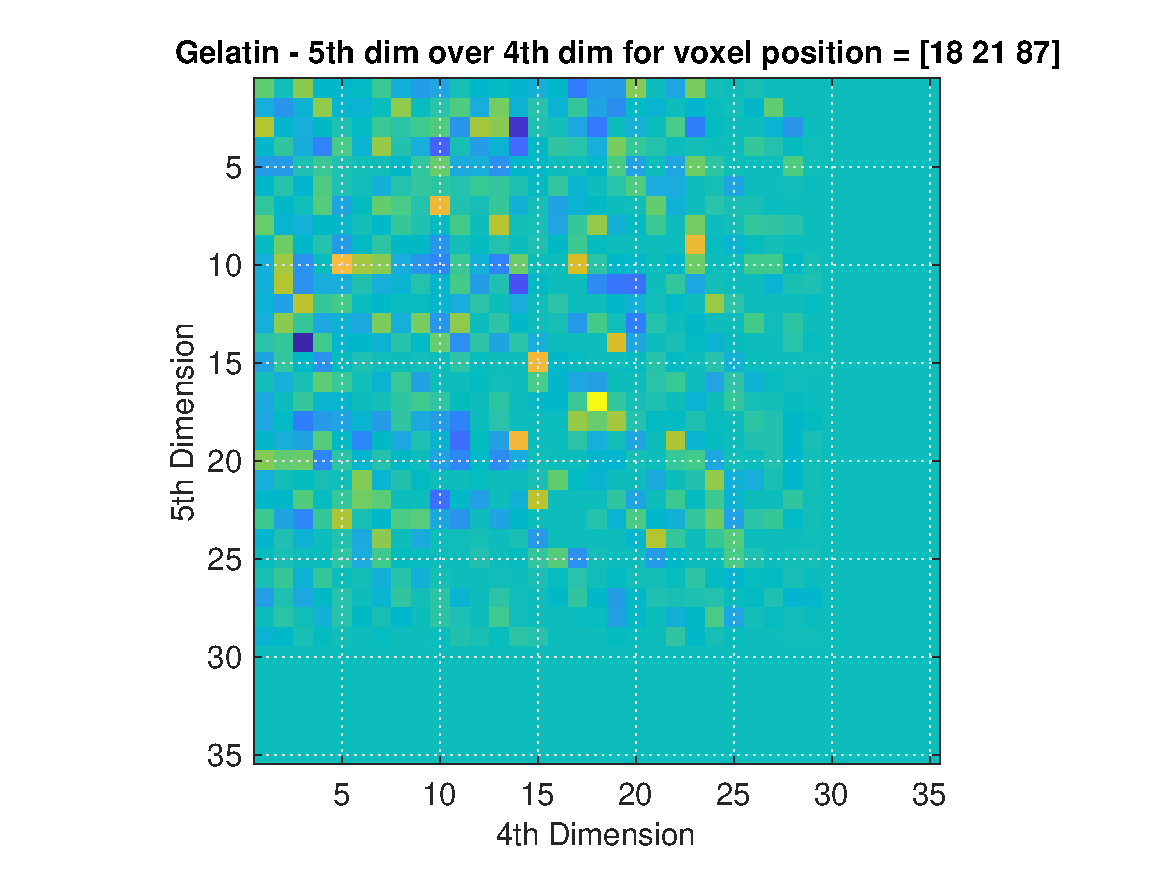
\includegraphics[width=1.09\textwidth]{Graphics/Results/skin_pulp_stone_5D_4D_Pulp.eps}
         \caption{Inside of gelatin. }
         \label{fig:res:5D_4D_skin_pulp_compare_pulp}
     \end{subfigure}
          \hfill
     \begin{subfigure}[b]{0.47\textwidth}
         \centering
         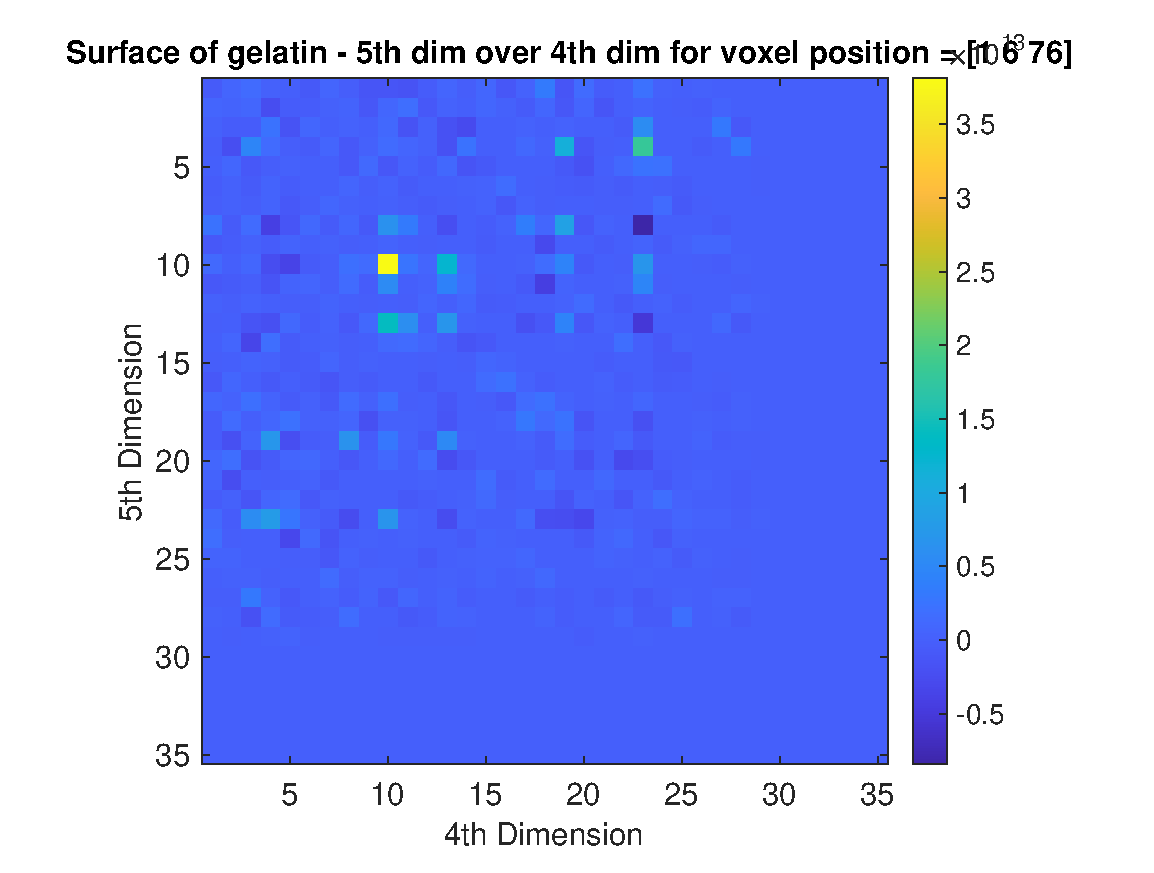
\includegraphics[width=1.09\textwidth]{Graphics/Results/skin_pulp_stone_5D_4D_Skin.eps}
         \caption{Surface of gelatin. }
         \label{fig:res:5D_4D_skin_pulp_compare_skin}
     \end{subfigure}
               \hfill
     \begin{subfigure}[b]{0.47\textwidth}
         \centering
         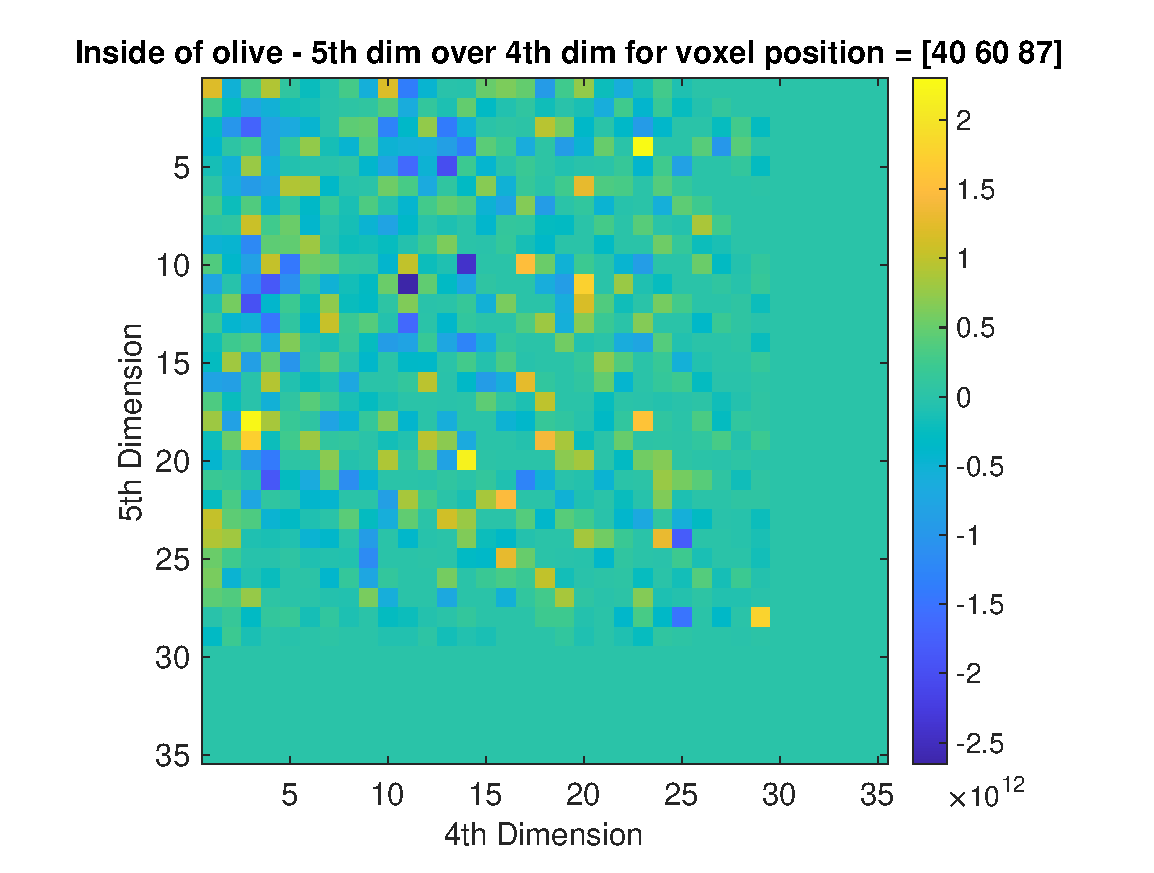
\includegraphics[width=1.09\textwidth]{Graphics/Results/skin_pulp_stone_5D_4D_Inside_Olive.eps}
         \caption{Inside of olive. }
         \label{fig:res:5D_4D_skin_pulp_compare_insideOlive}
     \end{subfigure}
        \caption{ 5D-over-4D representation of three different voxels in the reconstructed image. It is assumed that the olive skin and the surface of the gelatin block both have a prevailing specular reflection characteristic whereas the gelatin and the pulp of the olive are assumed to have predominantly diffuse properties. }
        \label{fig:res:5D_4D_skin_pulp_compare}
\end{figure}


 
In Figure \ref{fig:res:5D_4D_skin_pulp_compare} the voxel values are given in reference to the indices of the directional vectors that were used. For the quantitative analysis of these results the directional vectors first have to be organised in reference to their angular relation ship to each other. Section \ref{angular_directional_relation} introduces the so called graticule which represents the result in a physical context.

Since these 5D-over-4D results show features which can be used for the determination of the reflection characteristics they shall be explained qualitatively in the following.  


\medskip



In Figure \ref{fig:res:5D_4D_skin_pulp_compare_stone} we see the 5D-over-4D-representation for the voxel located at the surface of the olive. This plot can be used to make a first assertion about the tissue characteristics of the examined sample. The skin of the olive is assumed to have specular reflectivity properties since it has an relatively even surface. The surface of the gelatin block is also very even an therefore specular properties can be assumed. The 5D-over-4D representation for the surface of the gelatin can be seen in Figure \ref{fig:res:5D_4D_skin_pulp_compare_skin}.

Figure \ref{fig:res:5D_4D_skin_pulp_compare_insideOlive} and \ref{fig:res:5D_4D_skin_pulp_compare_pulp} show the voxel values for the inside of the olive and the gelatin block. Since these two samples are not located at even surfaces where no specular behaviour would be expected. 

The results for the specular behaviour are shown on the left side of Figure \ref{fig:res:5D_4D_skin_pulp_compare} whereas the plots on the right side are for the diffuse cases.

In this side by side comparison the distribution is noticeable. For the specular cases on the left there are some isolated high amplitude values surrounded by comparably low values. The diffuse cases on the right appear more evenly distributed and unorganised. 

In case of the surface of the gelatin block in Figure \ref{fig:res:5D_4D_skin_pulp_compare_skin} a symmetrical distribution of the values around the leading diagonal of the voxel matrix can be observed. This phenomenon can also be seen in Figure \ref{fig:res:5D_4D_skin_pulp_compare_stone} for the surface of the olive. In that case there are four dark values (e.g. negative amplitude) appear mirrored on the leading diagonal. 

The results for the diffuse case show a much more stochastic distribution of the values and no symmetrical distribution is recognisable.


\bigskip

The features of the 5D-over-4D representation can be used to extract information about the surface texture of different materials. One possibility for that would be the calculation of the deviation of all voxel values per 5D-4D representation and write them into the 3D volume. The results for that are shown in section \ref{chap:devi_image}.






\subsection{Angular relation between directional information}
\label{angular_directional_relation}


Until now the directional vectors could not be compared to each other properly. Their index was based on the order of their generation the angular relation between them was missing. A solution for this problem is presented in this section. A so called graticule is introduced. It is a representation of the azimuth and elevation of a spherical coordinate system in a 2 dimensional coordinate system. A simple example is shown in the following Figure:

\begin{figure}[H]
    \centering
    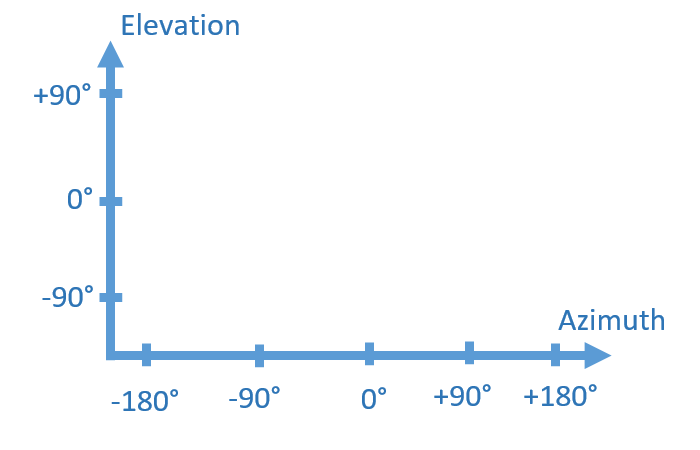
\includegraphics[width=0.76\textwidth]{Graphics/example_gradnetz.png}
    \caption{Basic representation of the graticule. The x-axis holds the information of the azimuth coordinate and the y-axis the information of the elevation. }
    \label{fig:gadnetz_example}
\end{figure}

With this representation the directional information of the single directional vectors now can be brought into a representative form so that the angular relationship between the data becomes visible. The 35 directional vectors that are used for the 5D reconstruction are shown in the following image: 

\begin{figure}[H]
    \centering
    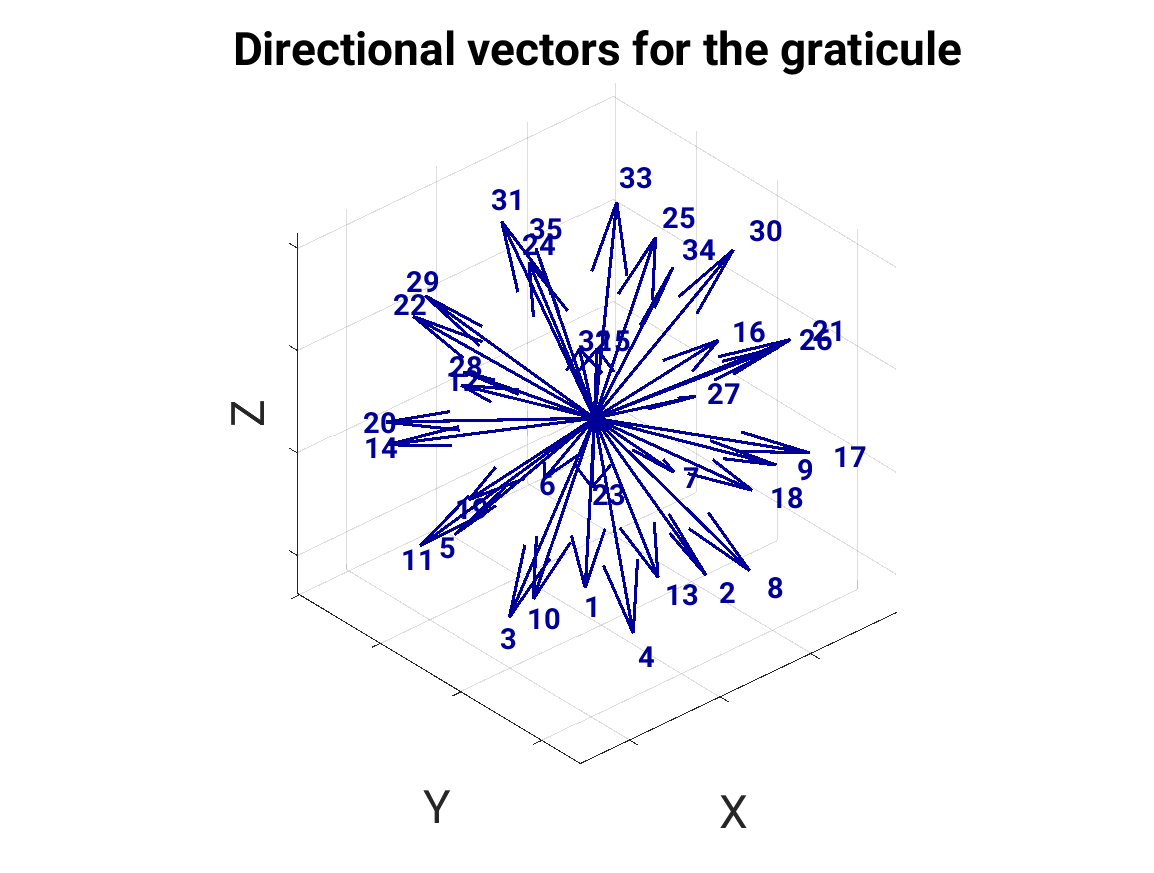
\includegraphics[width=0.76\textwidth]{Graphics/Results/gradnetz/directional_vectors_for_gradnetz.eps}
    \caption{The 35 directional vectors that shall be projected into the graticule. }
    \label{fig:gadnetz_directional_vectors}
\end{figure}

To transfer these directional vectors in the graticule the azimuth as well as the elevation is calculated for every direction vector. The resulting spherical coordinates are then plotted into the graticule. The values for the azimuth are plotted on the x-axis and the values for the elevation are assigned to the y-axis of the graticule. The result can be seen in the following image:

\begin{figure}[H]
    \centering
    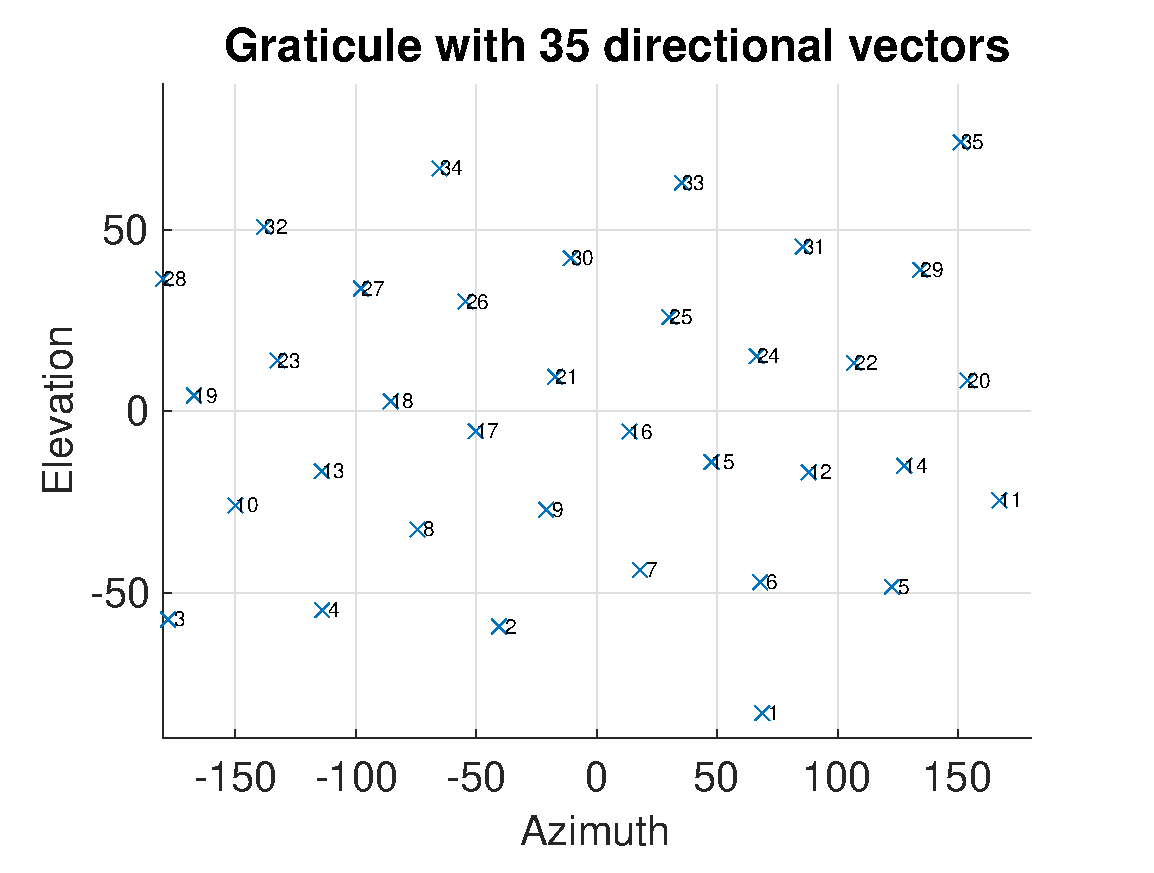
\includegraphics[width=0.76\textwidth]{Graphics/Results/gradnetz/graticule_35_vectors.eps}
    \caption{The 35 directional vectors now presented in the graticule. The units are given in degrees. }
    \label{fig:fertig_gradnetz}
\end{figure}

From the representation in Figure \ref{fig:fertig_gradnetz} now the directional vectors can be regarded with their angular relation to each other. This shall be shown in the following example. A test voxel is defined with the voxel coordinates $[70\, , \, 82\, , \, 91]$. The coordinates for the test voxel are plotted in Figure \ref{fig:gadnetz_location_testvoxel}.

\begin{figure}[H]
    \centering
    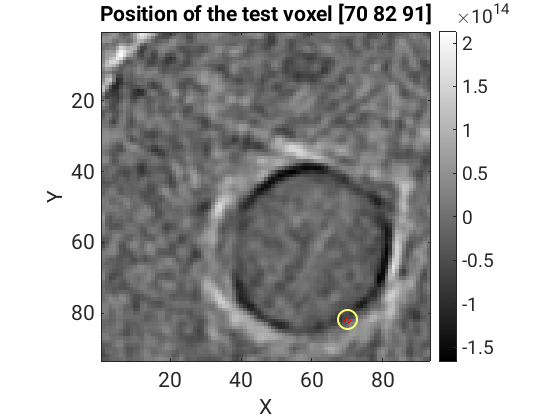
\includegraphics[width=0.76\textwidth]{Graphics/Results/gradnetz/positionof_test_voxel_for-gradnetz.png}
    \caption{Location of the test voxel $[70\, , \, 82\, , \, 91]$ for the graticule. }
    \label{fig:gadnetz_location_testvoxel}
\end{figure}

The test voxel was chosen on the surface of the olive. This surface is assumed to have specular properties as first results in section \ref{sec:res:eval_diff_tissue_type} indicated. 

\bigskip

For the generation of the following results the data set from section \ref{sec:input_data} were used. The reconstruction of the 5D image was performed with the orthogonality threshold method and with 35 directional vectors. The graticule with image data can be seen in Figure \ref{fig:gadnetz_with_values}.



\begin{figure}[H]
     \centering
     \begin{subfigure}[b]{0.77\textwidth}
                  \centering
         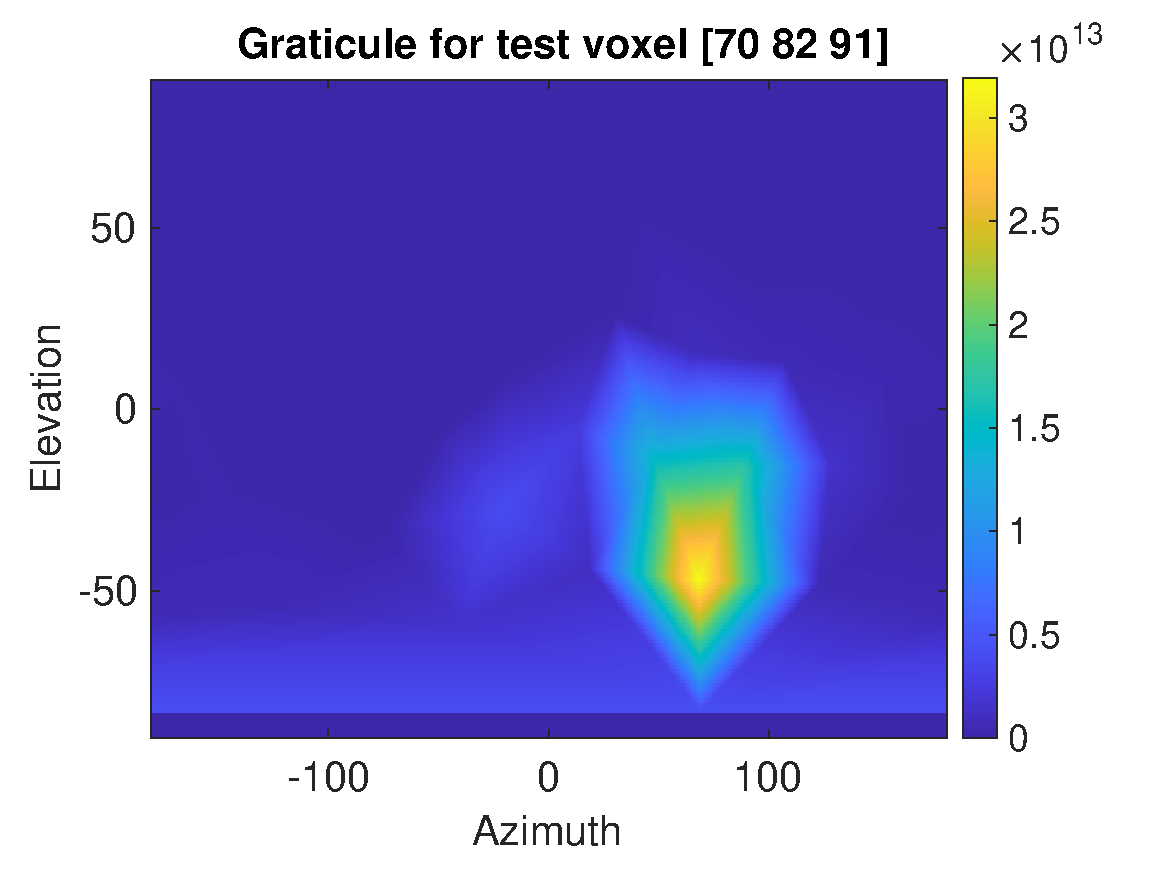
\includegraphics[width=1.09\textwidth]{Graphics/Results/gradnetz/graticule_with_values.eps}
         \caption{Graticule with the values of the receiver data for all directional vectors which have their origin at the emitter direction 12.}
         \label{fig:gadnetz_with_value_values}
     \end{subfigure}
     \hfill
     \begin{subfigure}[b]{0.77\textwidth}
         \centering
         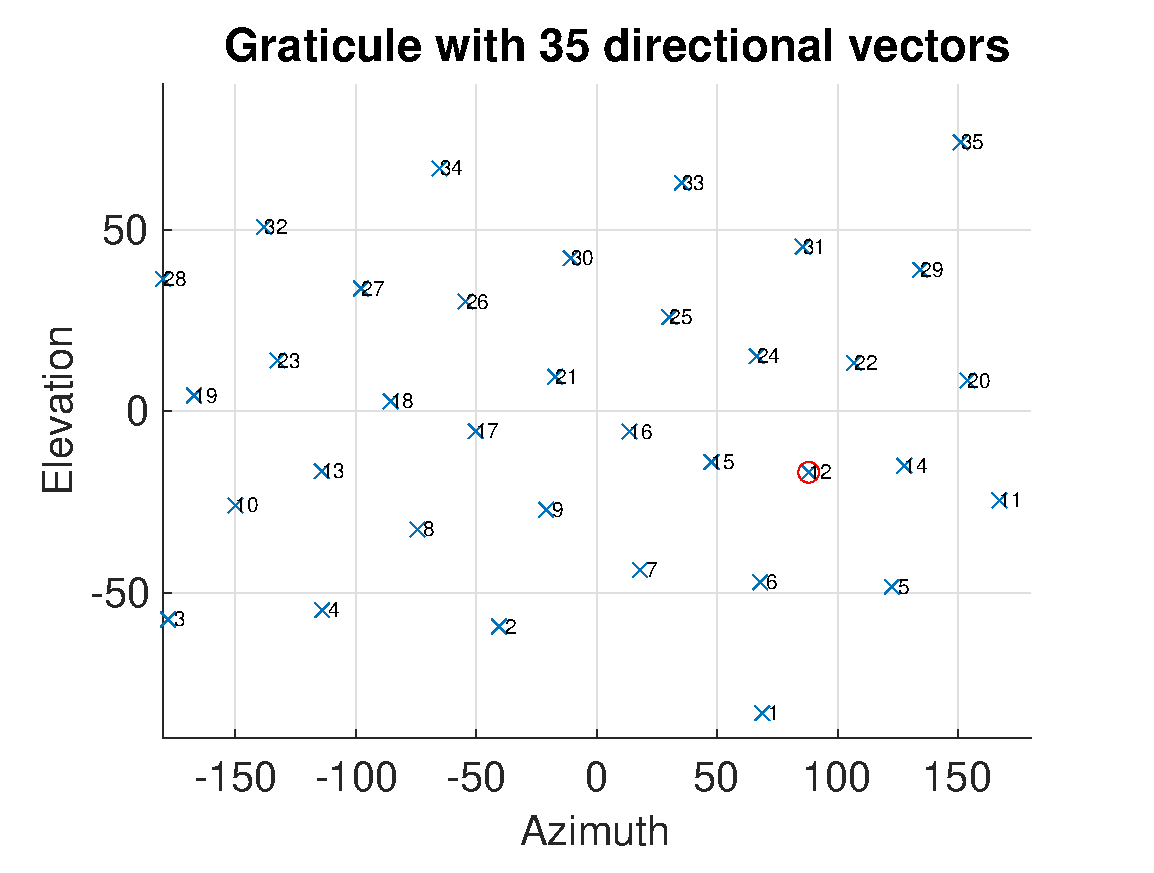
\includegraphics[width=1.09\linewidth]{Graphics/Results/gradnetz/graticule_35_vectors_emitter_12_active.eps}
         \caption{Graticule of the positions of the directional vectors. Vector 12 is marked red because the data of the graticule are used from the emitter direction 12.  }
         \label{fig:gadnetz_with_value_vecotrs}
     \end{subfigure}
        \caption{Influence of the \ac{sos} correction on the Deviation image.}
        \label{fig:gadnetz_with_values}
\end{figure}


For these results, the emitter direction was exemplarily chosen as 12. This means, that only the data is considered that was emitted from an emitter \ac{tas} that lay inside of the decision cone of directional vector 12. Furthermore, the receiver values for every direction are regarded. This means, that from all the data in the 5D image only the voxel values are regarded that originate from an emitter in direction 12. These voxel values then are placed into the graticule at the position of their corresponding receiver vectors and two dimensionally interpolated to create the image that we can see in Figure \ref{fig:gadnetz_with_value_values}. The colours of the figure represent the voxel value at that particular direction vector. The absolute value of the voxel values was chosen so that both positive and negative values of the \acp{ascan} are regarded. A bright structure is visible located at the position of the directional voxel 12. The structure results from the interpolation of the different voxel values located at the directional vectors surrounding vector 12. From the concentrated distribution of voxel values around the directional vector 12 the result can be interpreted as the result of a reflection on the surface of the olive with high specular properties. It remains to be examined how this structure changes if the test voxel is placed into other materials with different reflection properties and if the distribution of voxel values really allows for the classification of surface materials.  






\section{Deviation-imaging \& Max-imaging}
\label{chap:devi_image}

Since the final image of the reconstruction contains five dimensions the results are not easy to display in an comprehensible way. One option of displaying all the data of the five dimensions in one 3D volume was shown in Figure \ref{fig:res:summareized_bubble_ortho_image}. In this case the voxel values were averaged along the 4\textsuperscript{th} dimension and the 5\textsuperscript{th} dimension. This procedure results in a 3D image which is similar to the original \ac{usct}-images without any directional information.   

\bigskip

Another option for the representation of the data is the \textbf{deviation image}. It can be calculated from the 5D-over-4D representations and results in a three dimensional image. For each of the 5D-over-4D-images a standard deviation can be calculated. The results from section \ref{sec:res:eval_diff_tissue_type} showed a distinct pattern for tissue types with specular properties compared to tissue types with diffuse behaviour. For the specular kind there were some high peaks symmetrically distributed around the leading diagonal of the image whereas the diffuse tissue showed a more even distribution of value over the whole are of the image. With these observations in mind the standard deviation of a the 5D-over-4D characteristics for a specular scatterer should result in a higher value compared to the even distribution of the 5D-over-4D plot for the diffuse case. In the following Figure the Deviation image is shown next to the summarised image of the data set.


\begin{figure}[H]
     \centering
     \begin{subfigure}[b]{0.47\textwidth}
         \centering
        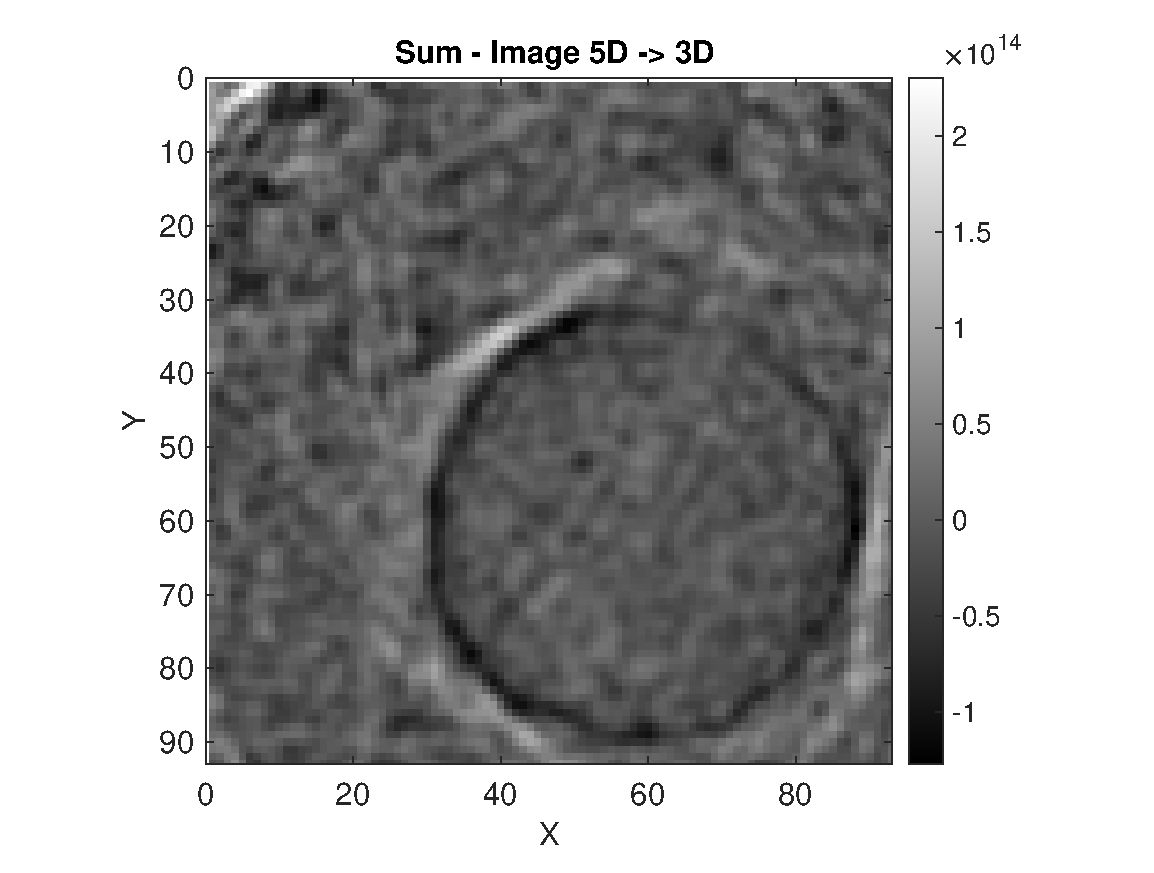
\includegraphics[width=1.09\linewidth]{Graphics/Results/Variance_Image/Variance_Ortho_slice_87_compare_5d_to_3d.eps}
         \caption{Slice thorough the 3D image which was constructed for the summation of the 4th and 5th dimension. }
         \label{fig:res:compare_normal_variance_normal}
     \end{subfigure}
     \hfill
     \begin{subfigure}[b]{0.47\textwidth}
         \centering
         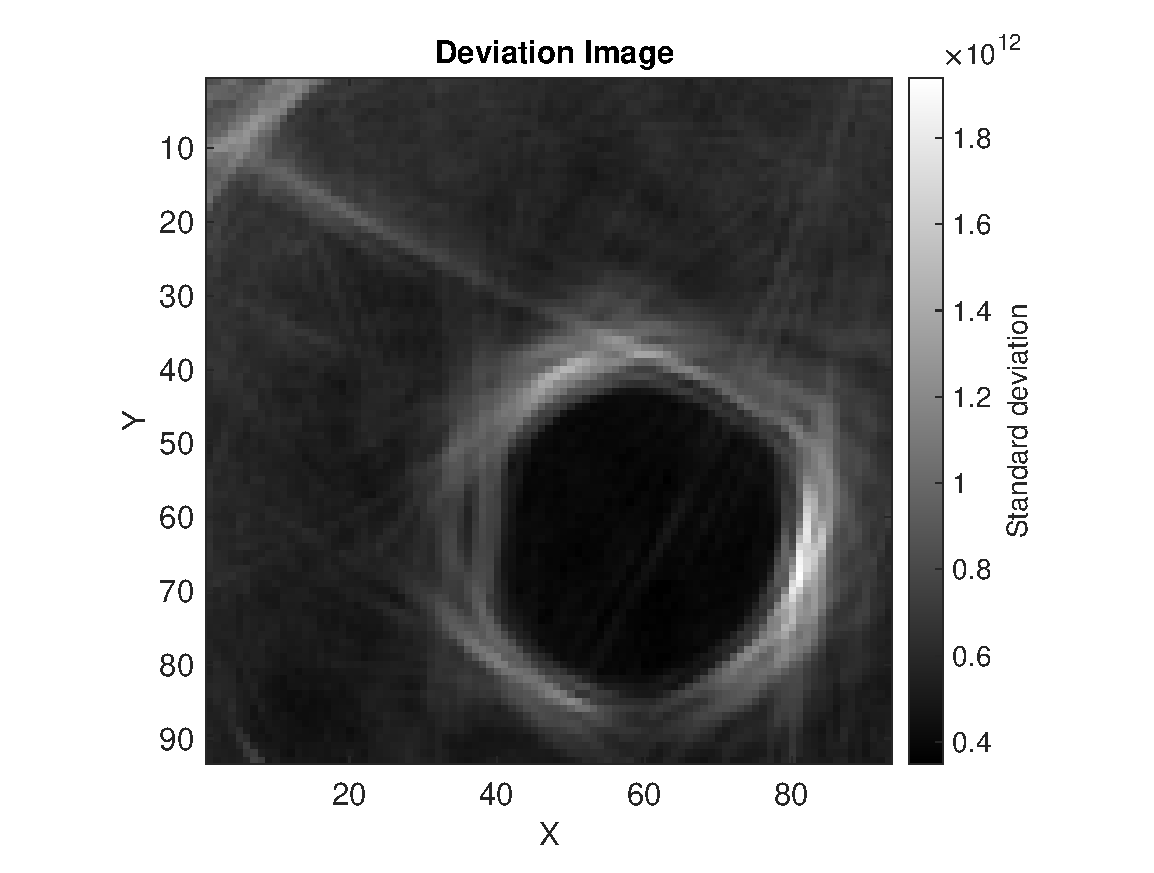
\includegraphics[width=1.13\textwidth]{Graphics/Results/Variance_Image/Variance_Ortho_slice_87.eps}
         \caption{Slice through the Deviation image. }
         \label{fig:res:compare_normal_variance_variance}
     \end{subfigure}
        \caption{Side by side comparison of the summarised 3D image to the Deviation image.}
        \label{fig:res:compare_normal_variance}
\end{figure}


Compared to the sum-image on the left the Figure \ref{fig:res:compare_normal_variance_variance} the deviation image shows a much higher contrast. The olive in the middle as well as the surface of the gelatin block in the top left corner are clearly visible. The speckle artefacts were suppressed and the background value is close to zero. 


In section \ref{sec:res:eval_diff_tissue_type} the data for four different test voxels with different reflection properties were shown. The deviation image shows that the voxel values for the voxels that were located on the surface of the olive and on the surface of the gelatin block have a high standard deviation (e.g. high brightness in image). These test voxel that were situated in the gelatin and on the inside of the olive a much lower deviation can be observed. 

\bigskip

With this method it could be shown that materials with a high diffuse reflectivity can be separated from low and diffuse reflecting materials. The voxels with high variance are highlighted in the deviation images and are easily distinguishable from the voxels with diffuse properties which appear much darker. 


\begin{figure}[H]
        \centering
    \begin{subfigure}[b]{0.61\textwidth}
         \centering
         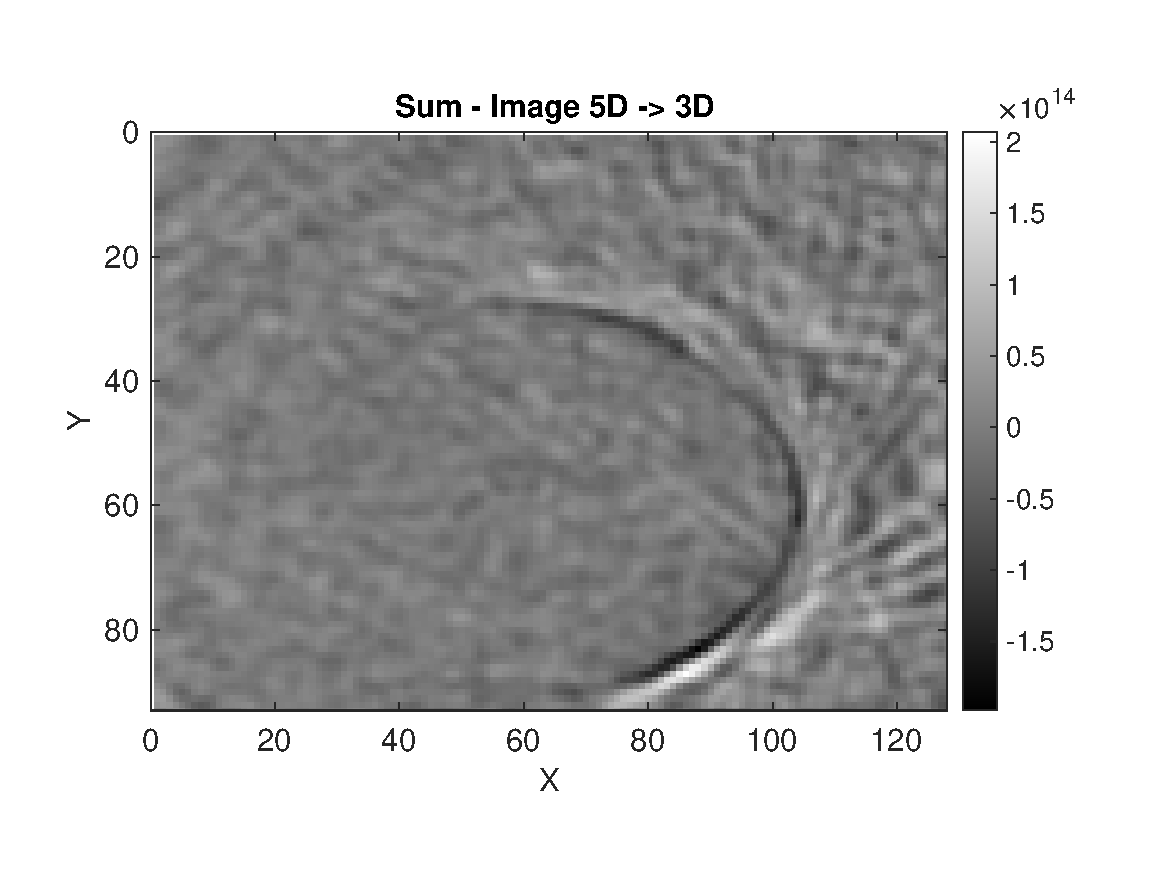
\includegraphics[width=1.13\textwidth]{Graphics/Results/Variance_Image/Variance_Ortho_slice_63_x_direkt_compare_5d_to_3d.eps}
         \caption{Summation image. }
         \label{fig:deviation_image_x_slice_normal}
     \end{subfigure}
     \hfill
    \begin{subfigure}[b]{0.61\textwidth}
        \centering
        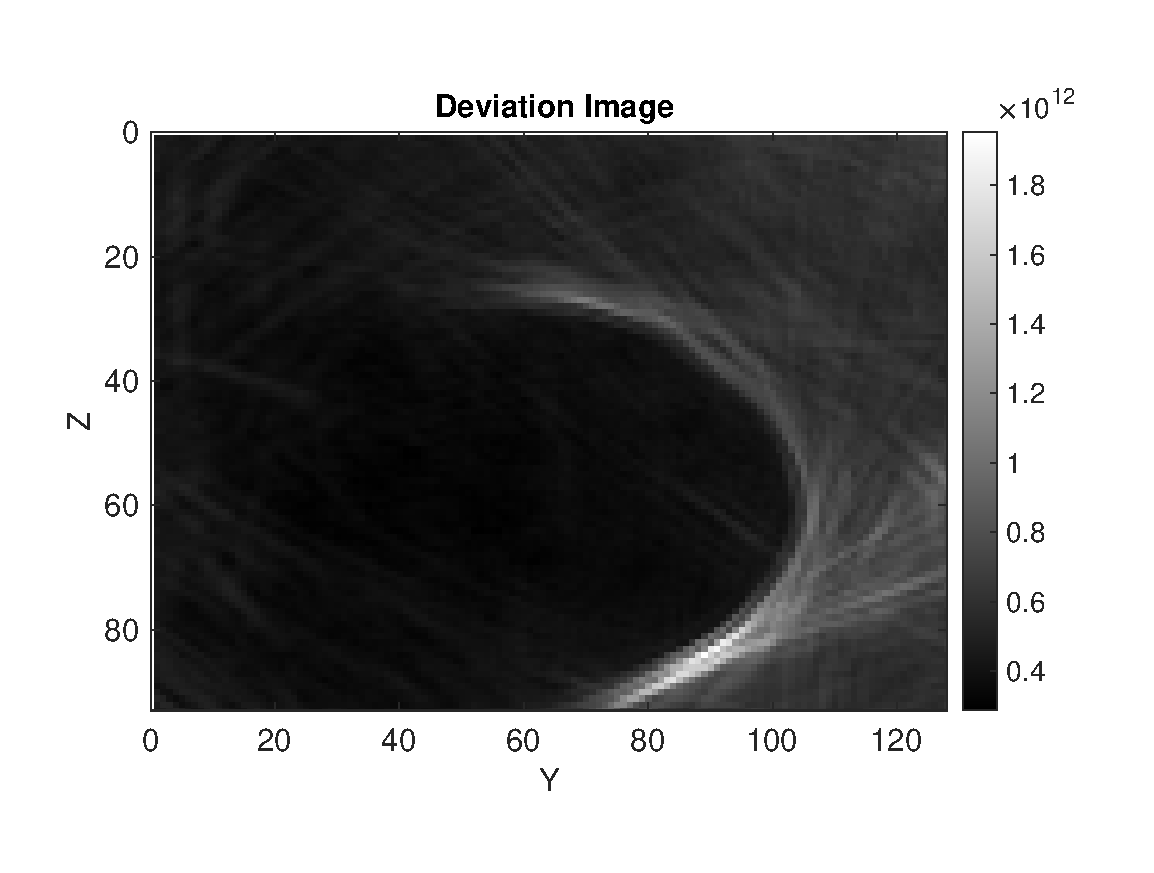
\includegraphics[width=1.13\textwidth]{Graphics/Results/Variance_Image/Variance_Ortho_slice_x_63.eps}
        \caption{Deviation image.}
        \label{fig:deviation_image_x_slice_deviation}
     \end{subfigure}
        \caption{Comparison of the Deviation image and the summation image. Sliced in x-direction. The oval in the middle of the image is the olive.}
        \label{fig:deviation_image_x_slice}
\end{figure}

In Figure \ref{fig:deviation_image_x_slice} the deviation image is shown from the side of the olive. This time the slices were made through the y-z-plain. Again, the edges of the olive are visible with higher contrast compared to the the summation image in Figure \ref{fig:deviation_image_x_slice_normal}. 


\bigskip
\bigskip



Using the \textbf{maximum values} of each of the 5D-4D-images leads to an alternative representation of the data. For the generation of the max image the highest peak of the 5D-4D-data is saved at the position of the corresponding voxel in the 3D image. The resulting max image is shown in the following figure \ref{fig:max_image}:


\begin{figure}[H]
    \centering
    \includegraphics[width=0.75\textwidth]{Graphics/Results/Variance_Image/Max_Ortho_slice_87.eps}
    \caption{Maximum image as a representation of the five dimensional data in 3D.}
    \label{fig:max_image}
\end{figure}




Figure \ref{fig:max_image} shows the maximum image with the same sectioning as the deviation image in Figure \ref{fig:res:compare_normal_variance_variance}. The results show the olive in the middle of the gelatin block as highlighted structure. In the specular case the ultrasonic pulses are reflected directly from the emitter direction into the receivers that lay in the same direction. Therefore, the pulses travel only a short distance and have little interaction with surrounding matter. For these cases the reflections cause a higher amplitude in the \ac{ascan} compared to a diffuse scattering where a big part of the energy is scattered into other directions. Therefore, the maximum imaging technique also leads to a highlighted representation of mainly specular tissue. 




      
\section{Influence of the speed of sound correction }
In this section the influence of the \ac{sos} correction on the images shall be shown. For the following results 14 directional vectors were used during the reconstruction. For the first comparison the sum images of the 5D reconstruction can be seen.


\begin{figure}[H]
     \centering
     \begin{subfigure}[b]{0.47\textwidth}
                  \centering
         \includegraphics[width=1.09\textwidth]{Graphics/Results/14_vecs_sos_vs_noSos/sum_14vecs_no_sos_z_direction.eps}
         \caption{Without \ac{sos} correction.}
         \label{sos:influence_sum_images_without}
     \end{subfigure}
     \hfill
     \begin{subfigure}[b]{0.47\textwidth}
         \centering
         \includegraphics[width=1.09\linewidth]{Graphics/Results/14_vecs_sos_vs_noSos/sum_14vecs_with_sos_z_direction.eps}
         \caption{With \ac{sos} correction. }
         \label{sos:influence_sum_images_with}
     \end{subfigure}
        \caption{Influence of the \ac{sos} correction on the summarised image of 5D reconstruction.}
        \label{sos:influence_sum_images}
\end{figure}

It is visible on the first glance that the influence of the artefacts could be reduced. The reason for the lower visibility of the noise is the higher amplitude of the voxel values where actual image information is stored. The Figure \ref{sos:influence_sum_images_with} shows a nearly two times higher amplitude compared to the image on the left. Therefore, the impact of the artefact could be reduced with the introduction of the \ac{sos} correction.

\bigskip

The 5D-over-4D images for the four different materials mentioned in section \ref{sec:input_data} are presented in the Figure \ref{fig:influence_sos_1} and \ref{fig:influence_sos_2}.
\begin{figure}[H]
     \centering
     \begin{subfigure}[b]{0.47\textwidth}
         \centering
         \includegraphics[width=1.02\linewidth,left]{Graphics/Results/14_vecs_sos_vs_noSos/5thdim_over4D_no_sos_pulp.eps}
         \caption{Without \ac{sos} correction. }
         \label{leer}
     \end{subfigure}
     \hfill
     \begin{subfigure}[b]{0.47\textwidth}
         \centering
         \includegraphics[width=1.02\textwidth]{Graphics/Results/14_vecs_sos_vs_noSos/5thdim_over4D_with_sos_pulp.eps}
         \caption{With \ac{sos} correction.}
         \label{leer}
     \end{subfigure}
          \hfill
     \begin{subfigure}[b]{0.47\textwidth}
         \centering
         \includegraphics[width=1.02\textwidth]{Graphics/Results/14_vecs_sos_vs_noSos/5thdim_over4D_no_sos_skin.eps}
         \caption{Without \ac{sos} correction.}
         \label{leer}
     \end{subfigure}
          \hfill
     \begin{subfigure}[b]{0.47\textwidth}
         \centering
         \includegraphics[width=1.02\textwidth]{Graphics/Results/14_vecs_sos_vs_noSos/5thdim_over4D_with_sos_skin.eps}
         \caption{With \ac{sos} correction.}
         \label{leer}
     \end{subfigure}
        \caption{Influence of the \ac{sos} correction on the 5D-over-4D-representation of reconstructed image with 14 directional vectors. The images on the left are reconstructed without the \ac{sos} correction. The results on the right are generated while considering the speed of sound.}
        \label{fig:influence_sos_1}
\end{figure}

These results are only compared qualitatively. It was mentioned in the section \ref{sec:res:eval_diff_tissue_type} that it is assumed that tissue types or materials with specular reflection characteristics have a symmetrical 5D-over-4D representation for that particular voxel. The symmetry can be enhanced by applying the \ac{sos} correction. The peak values are increased so that the artefacts have a smaller influence. This makes them more prominent in the 4D-over-5D representation and brings out the symmetry even more. 

\begin{figure}[H]
     \centering
      \hfill
     \begin{subfigure}[b]{0.45\textwidth}
         \centering
         \includegraphics[width=1.02\textwidth,right]{Graphics/Results/14_vecs_sos_vs_noSos/5thdim_over4D_no_sos_stone.eps}
         \caption{Without \ac{sos} correction.}
         \label{fig:influence_sos_2_a}
     \end{subfigure}
          \hfill
     \begin{subfigure}[b]{0.47\textwidth}
         \centering
         \includegraphics[width=1.02\textwidth]{Graphics/Results/14_vecs_sos_vs_noSos/5thdim_over4D_with_sos_stone.eps}
         \caption{With \ac{sos} correction.}
         \label{fig:influence_sos_2_b}
     \end{subfigure}
          \hfill
     \begin{subfigure}[b]{0.47\textwidth}
         \centering
         \includegraphics[width=1.02\textwidth]{Graphics/Results/14_vecs_sos_vs_noSos/5thdim_over4D_no_sos_inside_olive.eps}
         \caption{Without \ac{sos} correction.}
         \label{leer}
     \end{subfigure}
          \hfill
     \begin{subfigure}[b]{0.47\textwidth}
         \centering
         \includegraphics[width=1.02\textwidth]{Graphics/Results/14_vecs_sos_vs_noSos/5thdim_over4D_with_sos_inside_olive.eps}
         \caption{With \ac{sos} correction.}
         \label{leer}
     \end{subfigure}
        \caption{Influence of the \ac{sos} correction on the 5D-over-4D-representation of reconstructed image with 14 directional vectors. The images on the left are reconstructed without the \ac{sos} correction. The results on the right are generated while considering the speed of sound.}
        \label{fig:influence_sos_2}
\end{figure}


The biggest effect on the symmetry enhancement can be observed in Figures \ref{fig:influence_sos_2_a} and \ref{fig:influence_sos_2_b} for the skin of the olive. The result on the left shows first signs of a symmetrical distribution of the voxel values but has a lot of other superimposing components. The underlying noise could successfully be compensated by the application of the \ac{sos} correction and the symmetry could be brought about. 


\begin{figure}[H]
     \centering
     \begin{subfigure}[b]{0.47\textwidth}
              \centering
         \includegraphics[width=1.09\textwidth]{Graphics/Results/14_vecs_sos_vs_noSos/Deviation_14vecs_no_sos_z_direction.eps}
         \caption{Without \ac{sos} correction.}
         \label{leer}
     \end{subfigure}
     \hfill
     \begin{subfigure}[b]{0.47\textwidth}
         \centering
         \includegraphics[width=1.09\linewidth]{Graphics/Results/14_vecs_sos_vs_noSos/Deviation_14vecs_with_sos_z_direction.eps}
         \caption{With \ac{sos} correction. }
         \label{leer}
     \end{subfigure}
        \caption{Influence of the \ac{sos} correction on the deviation image.}
        \label{fig:influence_sos_on_deviation}
\end{figure}


The results for the deviation imaging were presented in section \ref{chap:devi_image}. This imaging method benefits also from the \ac{sos} correction. The comparison of the results with and without \ac{sos} correction are shown in Figure \ref{fig:influence_sos_on_deviation}. The contrast could be enhanced and the influence of noise reduced. 

\begin{figure}[H]
     \centering
     \begin{subfigure}[b]{0.47\textwidth}
                  \centering
         \includegraphics[width=1.09\textwidth]{Graphics/Results/14_vecs_sos_vs_noSos/Deviation_14vecs_no_sos_x_direction.eps}
         \caption{Without \ac{sos} correction.}
         \label{leer}
     \end{subfigure}
     \hfill
     \begin{subfigure}[b]{0.47\textwidth}
         \centering
         \includegraphics[width=1.09\linewidth]{Graphics/Results/14_vecs_sos_vs_noSos/Deviation_14vecs_with_sos_x_direction.eps}
         \caption{With \ac{sos} correction. }
         \label{leer}
     \end{subfigure}
        \caption{Influence of the \ac{sos} correction on the Deviation image.}
        \label{leer}
\end{figure}









%\section{Directional information used to reduce artefacts}
%\label{Reduce_artefacts}

%The directional information can be used to reduce the influence of the elipsoidal artefacts in the \ac{usct} image. The following example is shown for a 
\clearemptydoublepage


%!TEX root = ../thesis.tex
\chapter{Discussion \& Outlook}
\label{chap:discussion}


\section{Assessment of four and five dimensional approach}

During the reconstruction of an \ac{usct} image all the directional information of the transducers are lost. This is why Patrick Hucker \cite{PatrickHucker2014EvaluationRuckstreumodells} introduced a further dimension to his reconstructed images. The 4\textsuperscript{th} dimension can hold the directional information about the receiver directions or the emitter directions.

Why the 4\textsuperscript{th} dimension alone is not enough to characterise the reflection properties of different tissue types can be explained with a simple experiment:


\begin{figure}[H]
    \centering
    \includegraphics[width=0.56\textwidth]{Graphics/Diskussion/4D_not_enough.png}
    \caption{Experiment to prove that the 4\textsuperscript{th} dimensional approach is insufficient for analysing the reflection characteristics of a tissue. }
    \label{4D_sucks}
\end{figure}

In Figure \ref{4D_sucks} the aperture of the \ac{usct} device is shown. There are three emitters and three receivers. The green structure in the middle of the aperture is one big voxel which has an even surface and optimal specular reflection properties.

Because of the specularity of the surface, receiver 1 can only detect a pulse that originated from emitter 1. Analogously, receiver 2 can only detect the pulses from emitter 2 and receiver 3 can only receive a signal from emitter 3.

For the experiment three measurements are performed. For the first measurement only the first emitter is active and emits a pulse into the aperture. For the second measurement only the second and for the third measurement only the third emitter emits. During each of the three measurements all three receivers are active and measure the pressure. 

The recorded values are saved in a four dimensional image volume which is represented by the table in Figure \ref{table_2}: 

\begin{figure}[H]
    \centering
    \includegraphics[width=0.56\textwidth]{Graphics/Diskussion/4D_not_enough_table_2.png}
    \caption{Measured values for four dimensional direction information.}
    \label{table_2}
\end{figure}

In the table there is a column for each receiver but only one row for the emitters. This is why emitters 1,2 and 3 are summarised in the one row.

During the first measurement receiver 1 is the only receiver that detected a signal. For this measurement receiver 1 gets a red one. The remaining receivers get a red zero. The same goes for the second measurement: Receiver 2 receives a signal (green one in table), receivers 1 and 3 do not (green zeros in table). Analogously, for the third measurement only the third receiver is assigned the purple one whereas the other receivers are assigned the purple zero.

\bigskip

After the last measurement, the sum of the recorded signals result in a one in each receiver column. The information about what emitter was the origin of which signal is lost. If we would try to make an assumption about the reflection characteristics of this particular voxel, we would probably assume that the voxel reflected uniformly in all directions and therefore has to have a diffuse reflection characteristic.

\bigskip

Alternatively, we could have saved the measurement results into a 5\textsuperscript{th} dimension. This is represented by the table in Figure \ref{table_1}:

\begin{figure}[H]
    \centering
    \includegraphics[width=0.56\textwidth]{Graphics/Diskussion/4D_not_enough_table.png}
    \caption{Measured values for five dimensional direction information.}
    \label{table_1}
\end{figure}

From this table we can reconstruct the emitter receiver configuration under which a signal was detected. Since only the leading diagonal of the table is occupied it becomes clear that the voxel has to have a specular reflection characteristic. 

\bigskip


For the classification of a reflection characteristic it is therefore inevitable to analyse both the emitter and the receiver directions of a voxel. These information can only be preserved if a 5\textsuperscript{th} dimension is introduced to the reconstructed image. During this thesis the previous implementation of Patrick Hucker was extended and the tools for the analysis of the reflection characteristics. For the five dimensional approach the information of original 3D image is distributed into all the sub images for each 4D-5D combination. To compensate the reduced contrast of the resulting sub images a suitable visualisation technique is presented (compare section \ref{chap:max_devi}). 

\newpage

\section{Resolution of the discretisation of direction}

The resolution of the discretisation has to be considered for the characterisation of the reflective properties of a tissue. This can be explained with an example in Figure \ref{fig:resolution_of_segmentation}. The example shows two bell curves that represent two different reflection characteristics of a tissue. The wider curve represents a mixed reflectivity with specular and diffuse parts. The narrow green curve represents a near specular scatterer. The goal is to distinguish between both curves. In the sub-figures there are three different levels of the resolution of the directional information shown.


\begin{figure}[H]
     \centering
     \begin{subfigure}[b]{0.32\textwidth}
         \centering
        \fbox{\includegraphics[width=0.8\linewidth]{Graphics/zuwenigaufloesung.png}}
         \caption{Insufficient resolution of the discretisation.}
         \label{fig:resolution_of_segmentation_wenig}
     \end{subfigure}
     \hfill
     \begin{subfigure}[b]{0.32\textwidth}
         \centering
         \fbox{\includegraphics[width=0.8\textwidth]{Graphics/bessereaufloesung.png}}
         \caption{Better resolution of the discretisation.}
         \label{fig:resolution_of_segmentation_mittel}
     \end{subfigure}
     \hfill
     \begin{subfigure}[b]{0.32\textwidth}
         \centering
         \fbox{\includegraphics[width=0.8\textwidth]{Graphics/optimaleafloesung.png}}
         \caption{Optimal resolution of the discretisation.}
         \label{fig:resolution_of_segmentation_gut}
     \end{subfigure}
        \caption{Reflection characteristics of different surfaces and angle of incidence.}
        \label{fig:resolution_of_segmentation}
\end{figure}


In Figure \ref{fig:resolution_of_segmentation_wenig} the resolution of the directional information simply is not high enough to distinguish between both curves since they are both too narrow. The second solution shows a higher resolution of the discretisation of the directional information. The red lines are much closer to each other and the orange reflection characteristics can be analysed. To distinguish between the green and the orange curve the resolution is still insufficient. Figure \ref{fig:resolution_of_segmentation_gut} shows a near optimal solution for the problem. Both reflection characteristics could be distinguished. 

The introduction of the arbitrary directional segmentation allows to increase the resolution of the discretisation as desired and with that to increase the resolution of the segmentation. This is one of the main features that has been introduced during the thesis and allows the analysis of the different reflection characteristics. One of the challenges of the enhancement of the resolution of the segmentation is the increasing computation time. This issue was addressed by the introduction of a more efficient assignment method.






\section{Comparison of the assignment algorithms}
In section \ref{sec:index_ident} two approach for the assignment of the directional information were presented. The first method is the angle sorting approach which was introduced by Patrick Hucker.

It was extended from 4D to 5D during this thesis. The second method is the orthogonality threshold which was developed during this thesis. The main difference between both methods are the different decision criteria and the execution time. In section \ref{sec:index_ident} the different decision areas of both approaches were presented in detail. In the following the three decision criteria are compared:

\begin{figure}[H]
    \centering
    \includegraphics[width=0.76\textwidth]{Graphics/different_quality_assignment.png}
    \caption{Different decision areas of the angle sorting method (left) and the orthogonality threshold with enclosed decision area (middle) and with external decision area. }
    \label{angle_assignment_quality}
\end{figure}

For the \textbf{angle sorting} method there are fixed boundaries which correlate to the geometry of the configuration of directional vectors. For the 5D angle sorting method two different comparison vectors are assigned to the same directional vector. This can be seen in Figure \ref{angle_assignment_quality} on the left side. The comparison vector 1 is located at the boundary of the pentagon. Comparison vector 2 is located in one of the 'tips' of the pentagon where two boundaries meet. The distance from comparison vector 1 to the directional vector in the middle of the pentagon is smaller than the distance between comparison vector 2 and the directional vector. Still, both comparison vectors are assigned to the same directional vector. 
The decision area for the orthogonality threshold method is shown on the right side. The comparison vector 1 and 2 are both located on the boundary of the decision area. Both have the same distance to the directional vector 1 in the middle of the circle. 

Two comparison vectors that are located at the boundary of the same decision area can have a different angle to the comparison vector. For the angle sorting method both direction vectors may be assigned to the same directional vector. This leads to the conclusion that the angle sorting method has a varying quality of assignment. It can not be guaranteed that two comparison vectors that have the same angle to same directional vector are both assigned to the directional vector. 

\bigskip


The \textbf{orthogonality threshold} method treats all directional vectors equally and guarantees a constant quality of the assignment. If the threshold is chosen as the enclosed circle of the pentagon (compare Figure \ref{angle_assignment_quality} (middle)) some \acp{ascan} may be not regarded which results in a lower contrast of the image. On the other hand, this method leads to a distinct assignment.

The other possibility is to chose the decision areas to be overlapping. An example is given in Figure \ref{angle_assignment_quality} (right). For this case still a constant quality of the assignment can be assured and in addition to that all \acp{ascan} can be considered.

\bigskip

The other big difference between the two algorithms is their performance. While the angle sorting method iterates over every possible directional vector during the assignment process, the orthogonality threshold method needs only are previously calculated threshold for that one set of directional vectors and can compare the comparison vectors to this threshold. That increases the performance of the algorithm considerably. Both methods have to be executed multiple times during the reconstruction. To be precise for a full reconstruction there are $1.982x10^{16}$ calculations necessary where the assignment methods are involved. Therefore, this big difference in performance for more directional vectors makes the angle sorting approach to a bad choice. For small sets of directional vectors the impact may be not that big. With a rising number of directional vectors the threshold orthogonality method has its advantages in performance and the quality of the assignment process.  


Consequently, a trade-off has to be found between the advantages and disadvantages of the orthogonality method (uniqueness, contrast, vs. shorter computation time) and the angle search (potentially higher contrast vs. non-equal angular distribution of content and longer computation times). This thesis laid the groundwork which allows the analysis of the influence of the different decision criteria in the future with more data.





%\section{Advantages of looping implementation}

%-> Kein Meomory overflow

%\section{Alternative implementation of reconstruction}

%-> Directly in c++ code not as loop


\section{Interpretation of visualisation of the reflection characteristics}
\label{chap:max_devi}

For the comprehensible visualisation of the five dimensional data the deviation imaging and maximum imaging approach was presented. For each voxel in the measurement volume the directional data was interpreted and a three dimensional representation of the data was found. From the deviation and maximum images a first distinction between the specular and diffuse behaviour of a material was made possible. For the exact determination of different tissue types further evaluations are required. In particular the deviation approach lead to a suppression of the ellipsoidal artefacts in the image. These results might be suitable as input data for a machine learning algorithm which eventually could classify different tissues. Furthermore the relatively sharp representation of the surfaces could prove helpful for the segmentation of the tissue.


\section{Discussion of the implementation of the methods}

The multidimensional reconstruction was implemented in a way that two separate images are reconstructed for each directional vector. The biggest disadvantage of this method is the computation time of the reconstruction which increases linearly with the number of direction vectors. On the other hand, during the run time of the reconstruction algorithm of the old implementation, the assignment process needed to hold the whole image volume in the memory of the \acp{gpu}. This limit was overcome by calling the reconstruction multiple times and increasing the overall reconstruction time but also keeping the memory load of the \ac{gpu} constantly low. A next step would be to transfer the prototypically implemented MATLAB code into the CUDA kernel of the reconstruction. The implementation of the reconstruction for the five dimensional images was designed to be parallelisable and it can be partitioned arbitrarily.




\section{Conclusion \& Outlook}

The previous methods presented by Patrick Hucker \cite{PatrickHucker2014EvaluationRuckstreumodells} had inherent features that prevented the reconstruction of five dimensional volumes and with that made the successful classification of reflection characteristics improbable. The introduction of a 5\textsuperscript{th} dimension during this thesis brought us a big step closer to the classification of tissues by analysing the reflection characteristics. The inability to increase the resolution of the segmentation of the directional information arbitrarily was addressed during this thesis. A generalisation of the problem lead to new approach which allows to arbitrarily increase the resolution of the discretisation of the directional information. This new method lay the  groundwork for the detection of narrow reflection characteristics (e.g. specularity).

Moreover, the performance of the novel orthogonality threshold method was compared to the angle sorting method. The analysis concluded that the execution time per function call of the angle sorting method grew quadratically with the amount of directional vectors for the old method. This makes the old method unattractive for the assignment process with a high resolution of the discretisation. The execution time of the orthogonality method showed a linear behaviour with increasing numbers of direction vectors. This makes this method more suitable for high resolution applications. Non-overlapping decision areas were chosen for the current implementation of the orthogonality threshold to assure an unambiguous assignment to the directional vectors. The decision criteria could possibly be extended by weighting the assigned voxel values based on the orthogonality or distance to the directional vector. The influence of the different decision criteria on the resulting deviation and max images could be pursued in future.


The overall goal of this thesis was to provide insights into the reflection characteristics of different types of tissue and with these information increase the value of the reconstructed \ac{usct}-images. The distinguishing of tissue types with with near specular reflection properties from diffuse scatterers could be achieved with the introduction of the deviation imaging. This insight could prove helpful in future works for recognising different breast tissues and can possibly aid in the tumour detection.












%%!TEX root = ../thesis.tex
\chapter{Conclusion}
\label{chap:conclusion}

%\clearemptydoublepage


%%!TEX root = ../thesis.tex
\chapter{Outlook}
\label{chap:outlook}

%\clearemptydoublepage

\begin{appendix}
% uncomment the following line if you want to hide Appendix sections from TOC
%\addtocontents{toc}{\protect\setcounter{tocdepth}{0}}
%!TEX root = ../thesis.tex
\chapter{Additional Stuff 1}
\label{app:stuff1}

Whatever is not important enough to be included in the main document body but too important to leave out completely.

\end{appendix}

\clearemptydoublepage
\backmatter
\chapterstyle{default}
%%!TEX root = ./thesis.tex

\chapter{Symbolverzeichnis}
\markboth{Symbolverzeichnis}{Symbolverzeichnis}

%\section*{Notationsvereinbarung}
%\begin{tabular}{@{}ll@{}}
%Skalare & kursiv: $a, b, c,\dots$\\
%Vektoren& fett: $\mathbf{a, b, c,}\dots$\\
%Matrizen& fett, gro{\ss}: $\mathbf{A, B, C, \dots}$\\
%Mengen& kalligraphisch, gro{\ss}: $\mathcal{A, B, C}$\\
%Konstanten, Bezeichner& Kleinbuchstaben: $\mathrm{a, b, c}$\\
%
%\end{tabular}

%\section*{Symbole}
%\begin{tabularx}{\linewidth}{@{}ll@{}}
 \begin{longtable}{p{.27\textwidth}p{.67\textwidth}}
% \begin{tabular}{|p{.15\columnwidth}||p{.79\columnwidth}|}

\toprule
{\textbf{Formelzeichen}}							&
%%{\bf Einheit}							&
{\textbf{Bedeutung}} \\
\midrule
% \\
%\mbox{\em Lateinische Symbole} \\
%\\
$\Delta p$                      & Druckdifferenz\\
$\Delta p_{aw}$                 & Druckdifferenz in den Atemwegen\\
$\Delta p_{mus}$                & Druckdifferenz durch Muskelbewegung\\
$\Delta V$                      & Volumendifferenz\\



\bottomrule

\end{longtable}


%\addtocontents{toc}{Symbolverzeichnis}
\clearemptydoublepage
\iflists
  \listoffigures
  \clearemptydoublepage
  \listoftables
  \clearemptydoublepage
\fi

% References
{
 \ifafive
  \footnotesize
  \setlength{\bibsep}{1pt}
 \else
  \small
  \setlength{\bibsep}{2pt}
 \fi
 \bibliography{reduced,reference} % or refbase
 \clearemptydoublepage
}

\end{document}

